\chapter{Программная платформа ostis-систем}
\chapauthortoc{Зотов Н.В.\\Шункевич Д.В.}
\label{chapter_soft_platform}

\vspace{-7\baselineskip}

\begin{SCn}
	
\begin{scnrelfromlist}{автор}
	\scnitem{Зотов Н.В.}
	\scnitem{Шункевич Д.В.}
\end{scnrelfromlist}
	
\bigskip

\scntext{аннотация}{В данной главе формально описывается один из вариантов реализации программной платформы массовой коллективной разработки и эксплуатации интеллектуальных компьютерных систем нового поколения. В данной главе монографии детально иллюстрируется пример использования онтологического и компонентного подходов к разработке и описанию подкласса программных систем, являющихся системами автоматизации проектирования и реализации других программных систем. Данная глава является документацией программной платформы для ostis-системы, включающая описание особенностей, аналогов, а также достоинств и недостатков её реализации.}
	
\bigskip

\begin{scnrelfromlist}{подраздел}
	\scnitem{\ref{sec_soft_platform_problems}~\nameref{sec_soft_platform_problems}}
	\scnitem{\ref{sec_soft_platform_description}~\nameref{sec_soft_platform_description}}
	\scnitem{\ref{sec_soft_platform_sc_memory}~\nameref{sec_soft_platform_sc_memory}}
	\scnitem{\ref{sec_soft_platform_sc_memory_interface}~\nameref{sec_soft_platform_sc_memory_interface}}
	\scnitem{\ref{sec_soft_platform_file_memory}~\nameref{sec_soft_platform_file_memory}}
	\scnitem{\ref{sec_soft_platform_sc_server_subsystem}~\nameref{sec_soft_platform_sc_server_subsystem}}
	\scnitem{\ref{sec_soft_platform_sci_machine}~\nameref{sec_soft_platform_sci_machine}}
\end{scnrelfromlist}
	
\bigskip

\begin{scnrelfromlist}{ключевой знак}
	\scnitem{Программный вариант реализации ostis-платформы}
	\scnitem{Реализация sc-памяти в ostis-платформе}
	\scnitem{SCin-код}
	\scnitem{Программный интерфейс Реализации sc-памяти в ostis-платформе}
	\scnitem{Реализация файловой памяти ostis-платформы}
	\scnitem{SCfin-код}
	\scnitem{Реализация подсистемы взаимодействия ostis-платформы с внешней средой}
	\scnitem{SC-JSON-код}
	\scnitem{Реализация интерпретатора sc-моделей пользовательских интерфейсов}
\end{scnrelfromlist}
	
\bigskip

\begin{scnrelfromlist}{ключевое знание}
	\scnitem{Спецификация Программного варианта реализации ostis-платформы}
\end{scnrelfromlist}

\bigskip

\begin{scnrelfromlist}{библиографическая ссылка}
	\scnitem{\scncite{Sokolov2021}}
	\scnitem{\scncite{Iliadis2019}}
	\scnitem{\scncite{Dillon2007}}
	\scnitem{\scncite{Dillon2008}}
	\scnitem{\scncite{Ouksel1999}}
	\scnitem{\scncite{Neiva2016}}
	\scnitem{\scncite{Hagoort2009}}
	\scnitem{\scncite{Siekmann1984}}
	\scnitem{\scncite{Lu2022}}
	\scnitem{\scncite{Zapata2010}}
	\scnitem{\scncite{Bai2022}}
	\scnitem{\scncite{Neo4j}}
	\scnitem{\scncite{Robinson2015}}
	\scnitem{\scncite{Ballinger2009}}
	\scnitem{\scncite{Lenat1990}}
	\scnitem{\scncite{Lehmann2015}}
	\scnitem{\scncite{Gribova2016}}
	\scnitem{\scncite{Abramskiy2018}}
	\scnitem{\scncite{Vicknair2010}}
	\scnitem{\scncite{Klimanskaya2014}}
	\scnitem{\scncite{Chen2022}}
	\scnitem{\scncite{Gavrilova2001}}
	\scnitem{\scncite{Bashlyakov2010}}
	\scnitem{\scncite{Bashlyakov2013}}
	\scnitem{\scncite{Koronchik2013}}
	\scnitem{\scncite{Ivashenko2015}}
	\scnitem{\scncite{Shunkevich2018}}
	\scnitem{\scncite{Ostis-sc-machine2022}}
	\scnitem{\scncite{Belazzougui2010}}
	\scnitem{\scncite{Bayer1977}}
	\scnitem{\scncite{Tomasetti2021}}
	\scnitem{\scncite{Bhumij2018}}
	\scnitem{\scncite{Myers1992}}
	\scnitem{\scncite{Sadouski2022}}
\end{scnrelfromlist}

\end{SCn}


\section*{Введение в Главу \ref{chapter_soft_platform}~\nameref{chapter_soft_platform}}

До настоящего времени существует обширное множество различных решений в области автоматизации проектирования и разработки компьютерных систем (см. \scncite{Iliadis2019}), позволяющих решать задачи достаточно серьёзного уровня. Однако ни одна из таких систем не способна обеспечить платформенную независимость, а значит и семантическую совместимость и интероперабельность создаваемых компьютерных систем. Актуальность проблемы объясняется необходимостью создания компьютерных систем нового поколения, способных \myuline{быстро} и \myuline{качественно} решать задачи любого рода деятельности.

Современные компьютерные системы, а также средства автоматизации проектирования и разработки таких систем, обладают рядом значительных недостатков:

\begin{textitemize}
   \item Проектируемые программные компьютерные системы в большей мере остаются зависимыми от реализации конкретных платформ, на которых они проектируются, что, в свою очередь, приводит к существенным затратам на приведение в соответствие методов и средств проектирования систем в случае их перехода на новые платформы.
   \item Проектирование и разработка реализации конкретной системы ведётся при помощи разных методов и моделей проектирования программных компьютерных систем. Тем самым, описание целевого состояния системы и описание текущей реализации могут не соответствовать друг другу, а интеграция таких решений трудно достижима (cм. \scncite{Sokolov2021}).
   \item Место спецификации программных систем отводится на второй план, а иногда и вовсе не предусматривается проектом разработки конкретной компьютерной системы. Следовательно, увеличиваются затраты на поддержание процесса перманентного реинжиниринга таких систем (см. \scncite{Dillon2007}, \scncite{Dillon2008}).
   \item При разработке современных систем отсутствует понимание необходимости разработки и описания методов проектирования этих систем, в том числе описания процесса реализации, направлений использования и так далее. По этой причине новое поколение разработчиков программных компьютерных систем не используют уже имеющийся накопленный опыт, а изобретают одни и те же либо похожие решения.
   \item Отсутствуют единые универсальные инструментальные средства разработки и реинжиниринга других систем, позволяющие не только автоматизировать их проектирование, но и свести к минимуму саму разработку за счёт унификации моделей представления этих систем и наличия семантически мощной комплексной библиотеки многократно используемых компонентов.
   \item Даже узкоспециализированные программные компьютерные системы должны обладать хорошим уровнем интеллекта и хорошим уровнем обучаемости для расширения возможностей в решении более сложных задач. Программные компьютерные системы нового поколения в отличие от современных компьютерных систем, должны оперировать смыслом того, что они знают и обрабатывают: они должны понимать друг друга, находить точки соприкосновения и образовывать коллективы для решения задач любого класса (см. \scncite{Ouksel1999}, \scncite{Neiva2016}, \scncite{Lu2022}).
   \item Для эффективной реализации даже существующих моделей представления знаний и моделей решения трудно формализуемых задач современные компьютеры оказываются плохо приспособленными, что требует разработки принципиально новых платформ и компьютеров, обеспечивающих унификацию представления этих знаний (см. \scncite{Hagoort2009}, \scncite{Siekmann1984}).
\end{textitemize}

Обычно системы такого рода проектируются и разрабатываются для решения узких прикладных задач. В результате образуются системы с описанными выше проблемами. Так, большая часть из описанных проблем, к сожалению, не были решены при создании САПР, описанных в работах \scncite{Lenat1990}, \scncite{Gribova2016}, \scncite{Fillipov2016}.

При разработке спецификации таких систем важной задачей является задача выбора средств и методов проектирования будущей платформы разработки ostis-систем. Она должна обеспечивать.

\begin{textitemize}
    \item Однозначность интерпретации и представления логико-семантических моделей ostis-систем, обеспечиваемые используемым унифицированным языком представления знаний и онтологии проектирования платформ ostis-систем;
    \item Семантическую совместимость логико-семантических моделей ostis-систем и их компонентов между собой;
    \item Платформенную независимость реализуемых и интерпретируемых на ней логико-семантических моделей ostis-систем;
    \item Простоту и гибкость расширения своих функциональный возможностей и круга решаемых задач;
    \item Функциональную полноту для создания логико-семантических моделей ostis-систем за счёт наличия формальной методологии проектирования её реализации;
    \item Разделение обязанностей между компонентами (машинами) платформы.
\end{textitemize}

\section{Существующие подходы к проектированию систем автоматизации проектирования и реализации программных систем}
\label{sec_soft_platform_problems}

\begin{SCn}

\begin{scnrelfromlist}{ключевой знак}
	\scnitem{реляционная база данных}
	\scnitem{графовая база данных}
	\scnitem{SMILA}
	\scnitem{SYC}
	\scnitem{Neo4j}
\end{scnrelfromlist}

\begin{scnrelfromlist}{ключевой знак}
	\scnitem{Способы программной реализации ostis-платформы}
	\scnitem{Отличие реляционных баз данных от графовых баз данных}
\end{scnrelfromlist}

\end{SCn}

\bigskip

Реализация хранилищ данных, используемых в подавляющем большинстве компьютерные системы основываются на \textit{реляционной модели данных}. Примерами таких систем для обработки неструктурированных и слабоструктурированных данных являются платформы SMILA (SeMantic Information Logistic Architecture, Семантическая информационная логистическая архитектура), Teradata Aster Discovery Platform (см. \scncite{Ballinger2009}), реализующие реляционную, поколоночную и гибридную модели хранения записей в базе данных с массово-параллельной архитектурой MPP, платформа CYC (см. \cite{CycPlatform2022}), средства Semantic Web (см. \scncite{Lehmann2015}).

Однако, в настоящее время информационные системы подвергаются интенсивной интеллектуализации. В первую очередь, это вызвано повышением уровня сложности решаемых задач. Интеллектуализация информационных систем, как и любая технология разработки программных систем, требует учета слабоформализуемой, возможно не полностью определенной, нечеткой, темпоральной, пространственно-распределенной информации и, как следствия, получения структурированных, слабоструктурированных и неструктурированных данных. Увеличение числа интеллектуальных задач обработки больших объемов данных во всех сферах деятельности человека приводит к потребности создания универсальных средств хранения, представления и обработки мультиструктурированной информации.

Наличие таких задач стимулирует \myuline{переход от обычных баз данных к графовым аналогам}. Это объясняется не столько эффективностью организации памяти и обработки данных в графовых базах данных, сколько важностью представления конфигураций связей (то есть смысла) между ними (см. \scncite{Bai2022}). Подробное изъяснение принципов организации графовых данных в базах данных можно найти в работе авторов популярной графовой системой управления базами данных \textit{Neo4j} (см. \scncite{Robinson2015}, \scncite{Neo4j}).

Для общего понимания всей проблемы, связанной с представлением и обработкой данных и знаний рассмотрим несколько современных реализаций графовых моделей данных в виде программных продуктов. Любая из описанных ниже баз данных предназначена для удобного хранения и доступа к данным, представленным в виде графов сверхбольшой размерности. По организации памяти и процессу обработки данных графовые базы данных можно классифицировать на следующие виды:
\begin{textitemize}
    \item базы данных с локальным хранением и обработкой графов (Neo4j, HyperGraphDB, AllegroGraph);
    \item базы данных с распределенным хранением и обработкой данных (Horton, InfiniteGraph);
    \item базы данных в формате \scnqq{ключ-значение} (Trinity, CloudGraph, RedisGraph, VertexDB);
    \item документо-ориентированные базы данных (OrientDB);
    \item надстройки над SQL-ориентированными базами данных (Filament, G-store);
    \item графовые базы данных с моделью MapReduce (Pregel, Apache Giraph, GraphLab).
\end{textitemize}

С подробным описанием каждой из представленных баз данных можно ознакомиться в работах, посвящённых сравнению  реляционных и графовых баз данных \scncite{Abramskiy2018}, \scncite{Vicknair2010}, \scncite{Klimanskaya2014}, \scncite{Chen2022}.

Мотивация перехода от обычных графовых баз данных объясняется преимуществами организации модели памяти и обработки в них:
\begin{textitemize}
    \item Производительность обработки данных улучшается на единицу или более порядков при представлении данных в виде графовых структур, что объясняется свойствами самого графа. В отличие от реляционных баз данных, где производительность запросов с увеличением интенсивности запросов ухудшается по мере увеличения набора данных, производительность графовой базы данных имеет тенденцию оставаться относительно постоянными, даже когда набор данных растет. Это связано с тем, что обработка данных локализуется в некоторой части графа. В результате время выполнения каждого запроса равно пропорциональна только размеру части графа, пройденной для удовлетворения этого запроса, а не размеру всего графа.
    \item Графовые структуры имеют огромную выразительную силу. Графовые базы данных предлагают чрезвычайно гибкую модель данных и способ представления. Графовые структуры аддитивны, это обеспечивает гибкость добавления новых связей между данными, новые узлы и новые подграфы к уже существующей структуре, не нарушая её целостности и связности.
   	\item Многообразие форм представления данных минимизируется за счёт уменьшения количества синтаксических аспектов, учитываемых при хранении данных и использовании их в базах данных, поскольку графовые структуры данных позволяют записывать различные виды знаний одним и тем же способом.
\end{textitemize}

Как говорилось ранее, компьютерные системы нового поколения в силу своих свойств должны оперировать не просто данными, а знаниями. Чтобы понимать смысл знаний, необходимо представлять эти знания в понятной форме для каждого: и для человека, и для машины. Говоря об унификации представления всех видов знаний, важным считается использование графовых баз данных не просто как средств для хранения структурированных данных, а для хранения семантически целостных и связанных между собой знаний. В контексте проектирования компьютерных систем нового поколения будем говорить о базах знаний, проектируемых по принципам графовых баз данных.

Стоит также отметить, что акцент ставится не на разработку компьютерных систем поддержки проектирования других систем, а на разработку комплексных инструментальных средств поддержки автоматического проектирования интеллектуальных компьютерных систем нового поколения, управляемых знаниями. Такие инструментальные средства можно сравнивать с системами управления базами знаний \scncite{Naumov1991}, \scncite{Gavrilova2001}, \scncite{Bashlyakov2010}, \scncite{Bashlyakov2013}.

В основе \textit{ostis-платформы} должны лежать основополагающие принципы:
\begin{textitemize}
    \item Все тексты, представляемые на SC-коде являются графовыми конструкциями. Поэтому задача разработки \textit{Программного варианта реализации ostis-платформы} сводится к разработке средств хранения и обработки таких графовых конструкций. Другими словами, будущая платформа должна обеспечивать функционально полную и однозначную интерпретацию хранимых графовых конструкций.
    \item Проектирование платформы интерпретации sc-моделей ostis-систем, в том числе её компонентов, должно чётко специфицироваться и формулироваться в рамках моделей, методов и средств описания сложных систем, предлагаемых Технологией OSTIS. Именно онтологический подход к проектированию, эксплуатации и реинжиниринга такого подкласса компьютерных систем позволит эффективно и универсально разрабатывать другие ostis-системы самого различного назначения \scncite{Zapata2010}.
\end{textitemize}

Спецификация такого сложного программного объекта, как ostis-платформа, должна быть представлена на каком-то формальном языке представления знаний, в данном случае на SC-коде, поскольку она его должна хранить и обрабатывать. С точки зрения связи с самим SC-кодом, язык, который должен описывать \textit{программную реализацию ostis-платформы}, должен являться подъязыком SC-кода, то есть должен наследовать все свойства синтаксиса и денотационной семантики SC-кода, и метаязыком описания представления конструкций SC-кода в памяти программного эмулятора семантического ассоциативного компьютера. Такая модель представления спецификации программных компьютерных систем даёт безусловно сильные преимущества по сравнению с другими возможными вариантами представления спецификаций:
\begin{textitemize}
    \item Язык, тексты которого система хранит и обрабатывает, и язык спецификации того, как система представляет тексты первого языка в памяти самой себя, являются подмножествами одного и того же языка. Это упрощает не только становление понимание разработчика, который разрабатывает сложную программную систему, за счёт того, что форма представления обрабатываемого этой системой языка и языка её спецификации, унифицирована, но и позволяет открыть для этой системы новые функциональные возможности в познании самой себя. Таким образом, такой подход позволяет полностью реализовывать свойства интеллектуальной системы, например, рефлексивности.
    \item Нельзя проектировать и реализовывать интеллектуальные компьютерные системы на компьютерной системе, которая сама таковой не является. Представление спецификации системы в такой форме позволяет повысить уровень её интеллекта.
    \item Поскольку форма представления языка описания система унифицирована с языком, которые она обрабатывает, то нет необходимости в создании дополнительных средств для верификации и анализа работы системы.
\end{textitemize}

В таком случае, это позволяет не только уменьшить количество используемых средств при проектировании и реализации ostis-платформы, но и позволяет унифицировать информацию, хранимую в ostis-платформе и описывающую ostis-платформу, с целью использования этой информации в процессе эволюции компонентов ostis-платформы. При этом спецификация ostis-платформы остаётся платформенно-независимой, поэтому при смене одного варианта реализации ostis-платформы на другой подход к описанию ostis-платформы остаётся одним тем же.

\section{Принципы, лежащие в основе, и аналоги предлагаемого Программного варианта реализации ostis-платформы}
\label{sec_soft_platform_description}

\begin{SCn}
	
\bigskip

\begin{scnrelfromlist}{подраздел}
	\scnitem{\ref{sec_soft_platform_base_principles}~\nameref{sec_soft_platform_base_principles}}
	\scnitem{\ref{sec_soft_platform_doc_principles}~\nameref{sec_soft_platform_doc_principles}}
\end{scnrelfromlist}

\begin{scnrelfromlist}{ключевой знак}
	\scnitem{Программный вариант реализации ostis-платформы}
	\scnitem{Реализация памяти ostis-платформы}
	\scnitem{Документация Программного варианта реализации ostis-платформы}
	\begin{scnindent}
		\scnidtf{База знаний Программного варианта реализации ostis-платформы}
	\end{scnindent}
\end{scnrelfromlist}

\bigskip
	
\begin{scnrelfromlist}{ключевое знание}
	\scnitem{Обоснование разработки Программного варианта реализации ostis-платформы}
	\scnitem{Принципы, лежащие в основе Программного варианта реализации ostis-платформы}
	\scnitem{Принципы документирования Программного варианта реализации ostis-платформы}
	\scnitem{Отличие Программного варианта реализации ostis-платформы от других программных систем}
\end{scnrelfromlist}
	
\end{SCn}

Одним из путей, позволяющих осуществлять апробацию, развитие, а в ряде случаев и внедрение новых моделей и технологий вне зависимости от наличия соответствующих аппаратных средств является разработка программных моделей этих аппаратных средств, которые были бы функционально эквивалентны этим аппаратным средствам, но при этом интерпретировались на базе традиционной аппаратной архитектуры (в данной работе традиционной архитектурой будем считать архитектуру фон Неймана, как доминирующую в настоящее время). Очевидно, что производительность таких программных моделей в общем случае будет ниже, чем самих аппаратных решений, однако в большинстве случаев она оказывается достаточной для того, чтобы развивать соответствующую технологию параллельно с разработкой аппаратных средств и осуществления постепенного перевода уже работающих систем с программной модели на аппаратные средства.

Популярность и развитость графовых баз данных приводит к тому, что на первый взгляд целесообразным и эффективным кажется вариант реализации \textit{Программного варианта реализации ostis-платформы} на базе одного из таких средств. Однако, существует ряд причин, в силу которых это сделать невозможно. К ним относятся следующие:
\begin{textitemize}
	\item Для обеспечения эффективности хранения и обработки информационных конструкций определенного вида (в данном случае --- конструкций SC-кода, sc-конструкций), должна учитываться специфика этих конструкций. В частности, описанные в работе \scncite{Koronchik2013} эксперименты показали значительный прирост эффективности собственного решения по сравнению с существующими на тот момент.
	\item В отличие от классических графовых конструкций, где дуга или ребро могут быть инцидентны только вершине графа (это справедливо и для rdf-графов) в SC-коде вполне типичной является ситуация, когда sc-коннектор инцидентен другому sc-коннектору или даже двум sc-коннекторам. В связи с этим существующие средства хранения графовых конструкций не позволяют в явном виде хранить sc-конструкции (sc-графы). Данная проблема также решаема при переходе от неориентированного графа к орграфу \scncite{Ivashenko2015}.
	\item В основе обработки информации в рамках Технологии OSTIS лежит многоагентный подход (см. \ref{sec_mas}~\nameref{sec_mas}), в рамках которого агенты обработки информации, хранимой в sc-памяти (sc-агенты) реагируют на события, происходящие в sc-памяти и обмениваются информацией посредством спецификации выполняемых ими действий в sc-памяти \scncite{Shunkevich2018}. В связи с этим одной из важнейших задач является реализация в рамках \textit{Программного варианта реализации ostis-платформы} возможности подписки на события, происходящие в программной модели sc-памяти, которая на данный момент практически не поддерживается в рамках современных средств хранения и обработки графовых конструкций.
	\item SC-код позволяет описывать также внешние информационные конструкции любого рода (изображения, текстовые файла, аудио- и видеофайлы и так далее), которые формально трактуются как содержимое \textit{sc-элементов}, являющихся знаками \textit{внешних файлов ostis-системы}. Таким образом, компонентом \textit{Программного варианта ostis-платформы} должна быть реализация файловой памяти, которая позволяет хранить указанные конструкции в каких-либо общепринятых форматах. Реализация такого компонента в рамках современных средств хранения и обработки графовых конструкций также не всегда представляется возможной.
\end{textitemize}

По совокупности перечисленных причин было принято решение о реализации \textit{Программного варианта реализации ostis-платформы} \scnqq{с нуля} с учетом особенностей хранения и обработки информации в рамках Технологии OSTIS.

\begin{SCn}
\scnheader{Программный вариант реализации ostis-платформы}
\scnidtf{Реализация sc-машины}
\scnidtf{Программная платформа для ostis-систем}
\scnidtf{Базовая программная платформы для массового создания интеллектуальных компьютерных систем нового поколения}
\scnidtf{предлагаемый нами программный вариант реализации семантического ассоциативного компьютера}
\scnidtf{sc-machine}
\scniselement{специализированная ostis-платформа}
\begin{scnindent}
	\begin{scnreltolist}{ключевой знак}
		\scnitem{\ref{sec_interpreter_ostis_platform}~\nameref{sec_interpreter_ostis_platform}}
	\end{scnreltolist}
\end{scnindent}
\scniselement{web-ориентированный вариант реализации ostis-платформы}
\begin{scnindent}
    \scnidtf{вариант реализации платформы интерпретации sc-моделей компьютерных систем, предполагающий взаимодействие пользователей с системой посредством сети Интернет}
\end{scnindent}
\scniselement{многопользовательский вариант реализации ostis-платформы}
\begin{scnindent}
	\begin{scnreltolist}{ключевой знак}
		\scnitem{\ref{sec_interpreter_ostis_platform}~\nameref{sec_interpreter_ostis_platform}}
	\end{scnreltolist}
\end{scnindent}
\scniselement{многократно используемый компонент ostis-систем, хранящийся в виде файлов исходных текстов}
\begin{scnindent}
	\begin{scnreltolist}{ключевой знак}
		\scnitem{\ref{ostis_library_section}~\nameref{ostis_library_section}}
	\end{scnreltolist}
\end{scnindent}
\scniselement{неатомарный многократно используемый компонент ostis-систем}
\begin{scnindent}
	\begin{scnreltolist}{ключевой знак}
		\scnitem{\ref{ostis_library_section}~\nameref{ostis_library_section}}
	\end{scnreltolist}
\end{scnindent}
\scniselement{зависимый многократно используемый компонент ostis-систем}
\begin{scnindent}
	\begin{scnreltolist}{ключевой знак}
		\scnitem{\ref{ostis_library_section}~\nameref{ostis_library_section}}
	\end{scnreltolist}
\end{scnindent}
\scntext{адрес компонента}{https://github.com/ostis-ai/sc-machine}
\begin{scnrelfromset}{декомпозиция программной системы}
    \scnitem{Реализация памяти ostis-платформы}
    \scnitem{Реализация подсистемы взаимодействия с внешней средой с использованием языков сетевого взаимодействия}
    \scnitem{Реализация интерпретатора sc-моделей пользовательских интерфейсов}
    \scnitem{Реализация базового набора платформенно-зависимых sc-агентов и их общих компонентов}
\end{scnrelfromset}
\begin{scnrelfromset}{зависимости компонента}
    \scnitem{Реализация памяти ostis-платформы}
    \scnitem{Реализация подсистемы взаимодействия с внешней средой с использованием языков сетевого взаимодействия}
    \scnitem{Реализация интерпретатора sc-моделей пользовательских интерфейсов}
\end{scnrelfromset}
\end{SCn}

\subsection{Принципы, лежащие в основе Программного варианта реализации ostis-платформы}
\label{sec_soft_platform_base_principles}

\begin{SCn}
\scnheader{Программный вариант реализации ostis-платформы}
\begin{scnrelfromlistcustom}{принципы, лежащие в основе}
	\scnitemcustom{Текущий \textit{Программный вариант реализации ostis-платформы} является web-ориентированным, поэтому с этой точки зрения каждая \mbox{ostis-система} представляет собой web-сайт доступный онлайн посредством обычного браузера. Такой вариант реализации обладает очевидным преимуществом --- доступ к системе возможен из любой точки мира, где есть Интернет, при этом для работы с системой не требуется никакого специализированного программного обеспечения. С другой стороны, такой вариант реализации обеспечивает возможность параллельной работы с системой нескольких пользователей.}
	\scnitemcustom{Реализация является кроссплатформенной и может быть собрана из исходных текстов в различных операционных системах. В то же время, взаимодействие клиентской и серверной части организовано таким образом, что \mbox{web-интерфейс} может быть легко заменен на настольный или мобильный интерфейс, как универсальный, так и специализированный.}
	\scnitemcustom{Текущий вариант реализации ostis-платформы является специализированным, то есть не включает \textit{Реализацию интерпретатора базового языка SCP}. На текущем этапе разработки \textit{Программного вариант реализации ostis-платформы} все функционирующие ostis-системы являются платформенно-зависимыми. Данная проблема прежде всего связана с недостатками выбранной и реализованной модели управления доступа к sc-памяти, что не позволяет в полной мере создавать распределённые коллективы sc-агентов, работающих над sc-памятью.}
	\scnitemcustom{Ядром платформы является \textit{Реализация памяти ostis-платформы}, которая одновременно может взаимодействовать как с \textit{Реализацией интерпретатора sc-моделей пользовательских интерфейсов}, так и с любыми сторонними приложениями по соответствующим языкам сетевого взаимодействия (сетевым протоколам). С точки зрения общей архитектуры \textit{Реализация интерпретатора sc-моделей пользовательских интерфейсов} выступает как один из множества возможных внешних компонентов, взаимодействующих с \textit{Реализацией памяти ostis-платформы} по сети. Текущая \textit{Реализация интерпретатора sc-моделей пользовательских интерфейсов} является платформенно-зависимой, поскольку не в полной мере реализован интерпретатор базового языка SCP.}
	\scnitemcustom{Текущая \textit{Реализация памяти ostis-платформы} позволяет хранить и представлять sc-конструкции, с помощью которых описывается любая \textit{логико-семантическая модель ostis-систем}, внешние информационные конструкции, не принадлежащие \textit{SC-коду}, а также предоставлять различные уровни доступа для обработки этих конструкций. В контексте данного \textit{Программного варианта реализации ostis-платформы} \textit{Реализация памяти ostis-платформы} состоит из таких компонентов как: \textit{Реализация sc-памяти в ostis-платформе}, внутри которой представляются sc-конструкции \textit{логико-семантических моделей ostis-систем}, \textit{Реализация файловой памяти ostis-платформы}, внутри который представляются внешние информационные конструкции, не принадлежащие \textit{SC-коду}, то есть содержимое \textit{внутренних файлов ostis-системы}, но дополнительно описывающие, поясняющие и детализирующие sc-конструкции \textit{логико-семантических моделей ostis-систем}.}
	\scnitemcustom{Текущая \textit{Реализация памяти ostis-платформы}}
\end{scnrelfromlistcustom}
\end{SCn}

\begin{SCn}
	\scnheader{Реализация памяти ostis-платформы}
	\scnidtf{Реализация sc-памяти и файловой памяти ostis-платформы}
	\scniselement{многократно используемый компонент ostis-систем, хранящийся в виде файлов исходных текстов}
	\scniselement{неатомарный многократно используемый компонент ostis-систем}
	\scniselement{зависимый многократно используемый компонент ostis-систем}
	\scntext{адрес компонента}{https://github.com/ostis-ai/sc-machine/tree/main/sc-memory}
	\begin{scnrelfromset}{декомпозиция программной системы}
		\scnitem{Реализация sc-памяти в ostis-платформе}
		\scnitem{Реализация файловой памяти ostis-платформы}
	\end{scnrelfromset}
	\begin{scnrelfromset}{зависимости компонента}
		\scnitem{Библиотека методов и структур данных GLib}
		\scnitem{Библиотека методов и структур данных C++ Standart Library}
		\scnitem{Реализация sc-памяти ostis-платформы}
		\scnitem{Реализация файловой памяти ostis-платформы}
	\end{scnrelfromset}
\end{SCn}

Стоит отметить, что при переходе с \textit{Реализации памяти ostis-платформы} на её аппаратную реализацию \textit{файловую память ostis-системы} целесообразно будет реализовывать на основе традиционной линейной памяти (во всяком случае, на первых этапах развития \textit{семантического компьютера}). Текущий вариант \textit{Реализации памяти ostis-платформы} является открытым и доступен на \scncite{Ostis-sc-machine2022}.

\textit{Принципы, лежащие в основе Программного варианта реализации ostis-платформы} являются только базовыми, все компоненты, входящие в состав \textit{Программного варианта реализации ostis-платформы} имеют свои особенности реализации, а также аналоги, которые необходимо учитывать при реализации всей платформы.

\subsection{Принципы документирования Программного варианта реализации ostis-платформы}
\label{sec_soft_platform_doc_principles}

Перманентный реижиниринг компонентов текущего \textit{Программного варианта реализации ostis-платформы} обеспечивается открытой командой разработчиков, при этом каждый разрабатываемый компонент документируется согласно общепринятым принципам.

\begin{SCn}
\scnheader{Программный вариант реализации ostis-платформы}
\begin{scnrelfromlistcustom}{принципы документирования}
	\scnitemcustom{Вне зависимости от языка реализации каждого компонента \textit{Программного варианта реализации ostis-платформы}, спецификация каждого компонента включает спецификацию, непосредственно описанную в исходных файлах самого компонента, описывающую программный интерфейс этого компонента, а также спецификацию как части базы знаний ostis-платформы, детально описывающую реализацию этого компонента, в том числе используемые алгоритмы. При этом дублирование документации компонентов \textit{Программного варианта реализации ostis-платформы} категорически запрещается. Так, например, спецификация, непосредственно находящееся в исходном файле с реализацией самих компонентов, описывает особенности применения компонентов с точки зрения внешнего или внутреннего (то есть входящего в состав команды) разработчика, а спецификация, являющаяся частью sc-текста базы знаний \textit{Программного варианта реализации ostis-платформы}, дополнительно включает особенности, предлагаемые подходы к реализации, а также достоинства и недостатки входящих в состав компонентов.}
	\scnitemcustom{Каждый компонент \textit{Программного варианта реализации ostis-платформы} описывается средствами Технологии OSTIS, то есть на SC-коде, тексты которого она обрабатывает и хранит. Таким образом, это даёт возможности платформе анализировать своё состояние и способствовать поддерживать свой жизненный цикл без участия её разработчиков. \textit{Программный вариант реализации ostis-платформы} выступает полноценным субъектом, принимающим непосредственное участие в собственной разработке.}
	\scnitemcustom{Спецификация Программного варианта реализации ostis-платформы представляет собой sc-язык, то есть подъязык SC-кода, для которого уточнены синтаксис и семантика языка SC-кода. Вообще этот sc-язык можно представить в виде некоторого семейства более частных sc-языков, которые позволяют описывать:
	\begin{itemize}[labelsep=\tabsize-\bulletsize,leftmargin=\tabsize,label=$\bullet$]
		\item то, как sc-конструкции представляются внутри sc-памяти ostis-платформы;
		\item то, как информационные конструкции, которые не принадлежат SC-коду представляются внутри файловой памяти ostis-платформы;
		\item то, как различные подсистемы платформы, взаимодействуют между собой;
		\item то, какие методы и соответствующие им агенты взаимодействуют с sc-памятью ostis-платформы;
		\item то, как представляются и работают различного рода интерпретаторы sc-моделей (базы знаний, решателя, интерфейса);
		\item и так далее.
	\end{itemize}
	Такой подход позволяет без особых препятствий интегрировать описания различных компонентов, входящих в состав \textit{Программного варианта реализации ostis-платформы}, поскольку вся \textit{Документация Программного варианта реализации ostis-платформы} является её базой знаний с чётко выделенной иерархией предметных областей и онтологий (то есть sc-языков, описывающих её реализацию).}
	\scnitemcustom{Каждый разработчик \textit{Программного варианта реализации ostis-платформы} заботиться о перманентной поддержки не только состояния её компонентов, но и спецификации этих компонентов. Гарантом качественной \textit{Документации Программного варианта реализации ostis-платформы} является её коллектив разработчиков, способных не только понимать детали реализации ostis-платформы, но и способствовать к созданию взаимовыгодного сотрудничества для достижения поставленных целей.}
\end{scnrelfromlistcustom}
\end{SCn}

Данные принципы можно использовать при описании любых других программных компьютерных систем, в том числе тех систем, которые не реализуются на данной платформе.

\section{Реализация sc-памяти в Программной платформе ostis-систем}
\label{sec_soft_platform_sc_memory}

\begin{SCn}

\begin{scnrelfromlist}{подраздел}
	\scnitem{\ref{sec_soft_platform_scin_code}~\nameref{sec_soft_platform_scin_code}}
	\scnitem{\ref{sec_soft_platform_scin_code_alphabet_and_syntax}~\nameref{sec_soft_platform_scin_code_alphabet_and_syntax}}
	\scnitem{\ref{sec_soft_platform_scin_code_semantic}~\nameref{sec_soft_platform_scin_code_semantic}}
	\scnitem{\ref{sec_soft_platform_scin_code_problems}~\nameref{sec_soft_platform_scin_code_problems}}
\end{scnrelfromlist}

\begin{scnrelfromlist}{ключевой знак}
	\scnitem{Реализация sc-памяти в ostis-платформе}
	\scnitem{SCin-код}
	\begin{scnindent}
		\scnidtf{scin-текст}
	\end{scnindent}
	\scnitem{Алфавит SCin-кода\scnsupergroupsign}
	\scnitem{элемент sc-памяти}
	\scnitem{элемент sc-памяти, соответствующий sc-узлу}
	\scnitem{элемент sc-памяти, соответствующий sc-дуге}
	\scnitem{элемент sc-памяти, имеющий нулевой sc-адрес}
	\scnitem{sc-адрес элемента sc-памяти}
	\scnitem{sc-адрес элемента sc-памяти*}
	\scnitem{Синтаксис SCin-кода}
	\scnitem{Денотационная семантика SCin-кода}
\end{scnrelfromlist}

\end{SCn}

\bigskip

Под текущей \textit{Реализацией sc-памяти ostis-платформы} понимается компонент программной модели, осуществляющий хранение sc-конструкций и доступ к ним через программный интерфейс.

В рамках данного \textit{Программного варианта реализации ostis-платформы} \textit{sc-память} моделируется в виде набора \textit{сегментов}, каждый из которых представляет собой фиксированного размера упорядоченную последовательность \textit{элементов sc-памяти}, каждый из которых соответствует конкретному sc-элементу. В настоящее время каждый сегмент состоит из $2^{16}-1=65535$ \textit{элементов sc-памяти}. Каждый сегмент состоит из набора структур данных, описывающих конкретные \textit{sc-элементы} (элементов sc-памяти). Независимо от типа описываемого sc-элемента каждый \textit{элемент sc-памяти} имеет фиксированный размер (в текущий момент --- 36 байт), что обеспечивает удобство их хранения.

Выделение \textit{сегментов sc-памяти} позволяет, с одной стороны, упростить адресный доступ к \textit{элементам sc-памяти}, с другой стороны --- реализовать возможность выгрузки части sc-памяти из оперативной памяти на файловую систему при необходимости. Во втором случае сегмент sc-памяти становится минимальной (атомарной) выгружаемой частью sc-памяти. Механизм выгрузки сегментов реализуется в соответствии с существующими принципами организации виртуальной памяти в современных операционных системах.

Максимально возможное число сегментов ограничивается настройками программной реализации sc-памяти (в настоящее время по умолчанию установлено количество $2^{16}-1=65535$ sc-сегментов, но в общем случае оно может быть другим). Таким образом, технически максимальное количество хранимых sc-элементов в текущей реализации составляет около $4.3 \times 10^{9}$ sc-элементов. По умолчанию все сегменты физически располагаются в оперативной памяти, если объема памяти не хватает, то предусмотрен механизм выгрузки части sc-сегментов на жесткий диск (механизм виртуальной памяти).

Текущий вариант \textit{Реализации sc-памяти в ostis-платформе} предполагает возможность сохранения состояния (слепка) памяти на жесткий диск и последующей загрузки из ранее сохраненного состояния. Такая возможность необходима для перезапуска системы, в случае возможных сбоев, а также при работе с исходными текстами базы знаний, когда сборка из исходных текстов сводится к формированию слепка состояния памяти, который затем помещается в \textit{Реализации sc-памяти в ostis-платформе}.

\begin{SCn}
\scnheader{Реализация sc-памяти в ostis-платформе}
\scnidtf{Программный вариант реализации графодинамической ассоциативной памяти в Программной платформе ostis-систем}
\scniselement{реализация sc-памяти}
\scniselement{многократно используемый компонент ostis-систем, хранящийся в виде файлов исходных текстов}
\scniselement{неатомарный многократно используемый компонент ostis-систем}
\scniselement{зависимый многократно используемый компонент ostis-систем}
\scnrelto{программная модель}{sc-память}
\begin{scnindent}
	\begin{scnreltolist}{ключевой знак}
		\scnitem{\ref{chapter_interpreter}~\nameref{chapter_interpreter}}
	\end{scnreltolist}
    \scnrelto{семейство подмножеств}{сегмент sc-памяти}
    \begin{scnindent}
        \scnidtf{страница sc-памяти}
        \scnrelto{семейство подмножеств}{элемент sc-памяти}
    \end{scnindent}
\end{scnindent}
\begin{scnrelfromset}{зависимости компонента}
    \scnitem{Библиотека методов и структур данных GLib}
    \scnitem{Библиотека методов и структур данных C++ Standart Library}
\end{scnrelfromset}
\begin{scnrelfromlist}{используемый язык программирования}
    \scnitem{C}
    \scnitem{C++}
\end{scnrelfromlist}
\begin{scnrelfromlist}{внутренний язык}
    \scnitem{SCin-код}
\end{scnrelfromlist}
\end{SCn}

В общем случае \textit{sc-память} может быть реализовано по-разному. Так, например, другой вариант sc-памяти ostis-платформы можно реализовать при помощи программной реализации памяти платформы \textit{Neo4j}. Отличие такого возможного варианта реализации sc-памяти от текущего состоит в том, что хранение графовых конструкций и управление потоков операций над ними должно осуществляться в большей мере средствами, предоставляемыми платформой \textit{Neo4j}, в том же время представление графовых конструкций должно реализовываться по-своему, поскольку зависит от синтаксиса SC-кода.

Такую модель sc-памяти достаточно просто описывать на sc-языке, то есть на подъязыке SC-кода. Такой язык позволяет описывать то, как внутри памяти ostis-платформы представляются тексты языка, на этом же языке. При этом соблюдается не только унификация представления информации, обрабатываемой ostis-платформой, и информации, описывающую саму ostis-платформу, но и даются возможности для расширения и использования языка в процессе эволюции ostis-платформы и её компонентов, в том числе в процессе эволюции \textit{Реализации sc-памяти в ostis-платформе}.

\subsection{Формальная спецификация sc-языка внутреннего представления sc-конструкций в sc-памяти ostis-платформы}
\label{sec_soft_platform_scin_code}

Раннее упоминалось об sc-языках, которые используются при описании компонентов текущего \textit{Программного варианта реализации ostis-платформы}. Одним из таких языков будем называть sc-языком внутреннего представления конструкций SC-кода, или, кратко, \textit{SCin-кодом (Semantic Сode interior)}. Sc-память текстов SC-кода (как некоторую абстрактную модель, по которой можно реализовать sc-память ostis-платформы) можно рассматривать как подмножество scin-текста.

\begin{SCn}
\scnheader{SCin-код}
\scnidtf{Semantic Code interior}
\scnidtf{Язык внутренного смыслового представления SC-кода внутри памяти ostis-системы}
\scnidtf{метаязык описания представления SC-кода внутри памяти ostis-системы}
\scntext{часто используемый неосновной внешний идентификатор sc-элемента}{scin-текст}
\begin{scnindent}
    \scniselement{имя нарицательное}
\end{scnindent}
\scniselement{абстрактный язык}
\scniselement{метаязык}
\scniselement{sc-язык}
\scnsubset{SC-код}
\scnsuperset{sc-память}
\end{SCn}

\subsection{Cинтаксис SCin-кода}
\label{sec_soft_platform_scin_code_alphabet_and_syntax}

\textit{Синтаксис SCin-кода} задается: (1) \textit{Алфавитом SCin-кода}, (2) отношением инцидентности \textit{sc-адрес элемента sc-памяти*}. Важно отметить, что \textit{Синтаксис SCin-кода}, как и синтаксис других sc-языков, является подмножеством \textit{Синтаксиса SC-кода}, то есть \textit{Алфавит SCin-кода\scnsupergroupsign}, а также отношение инцидентности \textit{sc-адрес элемента sc-памяти*} являются подмножествами \textit{Алфавит SC-кода\scnsupergroupsign} и отношений инцидентности \textit{SC-кода} \textit{см. \ref{sec_semantic_classification_sc-elements}~\nameref{sec_semantic_classification_sc-elements}} соответственно, при этом правила \textit{Синтаксиса SCin-кода} включают правила \textit{Синтаксиса SC-кода} и правила, которые уточняют ньюансы \textit{Синтаксиса SCin-кода}.

\begin{SCn}
\scnheader{Алфавит SCin-кода\scnsupergroupsign}
\scnidtf{синтаксический тип элемента sc-памяти}
\scnidtf{Множество типов элементов sc-памяти}
\scnrelto{алфавит}{SCin-код}
\begin{scneqtoset}
    \scnitem{элемент sc-памяти, соответствующий sc-узлу}
    \scnitem{элемент sc-памяти, соответствующий sc-дуге}
    \scnitem{элемент sc-памяти, имеющий нулевой sc-адрес}
    \begin{scnindent}
        \scniselement{синглетон}
    \end{scnindent}
\end{scneqtoset}
\end{SCn}

\textit{Алфавит SCin-кода\scnsupergroupsign} состоит из трёх синтаксически выделяемых типов элементов sc-памяти: элемента sc-памяти, соответствующего sc-узлу общего вида, элемента sc-памяти, соответствующего sc-дуге общего вида и элемента sc-памяти, имеющего нулевой sc-адрес. Такой алфавит не только позволяет задавать в памяти минимальный набор объектов с которым можно производить вычислительные операции, но и, при необходимости, удобен для расширения. Так, например, в даннный алфавит языка можно расширить, добавив в его \textit{элемент sc-памяти, соответствующий внутреннему файлу ostis-системы} либо \textit{элемент sc-памяти, соответствующий sc-ребру}.

\begin{SCn}
\scnheader{элемент sc-памяти}
\scniselement{sc-элемент}
\scnidtf{элемент sc-памяти, соответствующий sc-элементу}
\scnidtf{ячейка sc-памяти}
\scnidtf{образ sc-элемента в рамках sc-памяти}
\scnidtf{структура данных, каждый экземпляр которой в рамках sc-памяти соответствует одному sc-элементу}
\scnrelfrom{разбиение}{Алфавит SCin-кода\scnsupergroupsign}
\end{SCn}

Отношение \textit{sc-адрес элемента sc-памяти*} определяется как взаимно однозначное соответствие, первым компонентом каждой ориентированной пары которого является некоторый элемент sc-памяти, соответствующей некоторому sc-элементу, а вторым компонентом является sc-адрес этого \textit{элемент sc-памяти}. То есть каждый \textit{элемент sc-памяти} имеет уникальный \textit{sc-адрес} как некоторый идентификатор, с помощью которого определяется \textit{уникальность элемента sc-памяти}.

Каждый элемент sc-памяти в текущей реализации может быть однозначно задан его sc-адресом, состоящим из номера sc-сегмента и номера \textit{элемента sc-памяти} в рамках sc-сегмента. Таким образом, \textit{sc-адрес} служит уникальными координатами \textit{элемента sc-памяти} в рамках \textit{Реализации sc-памяти}.

Для каждого sc-адреса можно взаимно однозначно поставить в соответствие некоторый хэш, полученный в результате применения специальной хэш-функции над этим sc-адресом. Хэш является неотрицательным целым числом и является результатом преобразования номера sc-сегмента sc-памяти si, в котором располагается sc-элемент, и номера этого sc-элемента sc-памяти ei в рамках этого сегмента si. В рамках sc-памяти используется единственная хеш-функция для получения хеша sc-адреса sc-элемента и задаётся как $f(si, ei) = si << 16 | ei \& 0xffff$, где операция $<<$ --- операция \textit{Битового сдвига влево*} левого аргумента на количество единиц, заданное правым аргументом, относительно этой операции, операция $|$ --- операция \textit{Битового сложения*}, операция $\&$ --- операция \textit{Битового умножения*}, число $0xffff$ --- число 65535, представленное в шестнадцатеричном виде и обозначающее максимальное количество sc-элементов в одном сегменте sc-памяти. Числовое выражение \textit{sc-адреса} является 32-битовым целым числом.

\begin{SCn}
	\scnheader{sc-адрес элемента sc-памяти}
	\scnidtf{адрес элемента sc-памяти, соответствующего заданному sc-элементу, в рамках текущего состояния реализации sc-памяти в составе программной модели sc-памяти}
	\scniselement{32-битовое целое число}
\end{SCn}

В рамках любой \textit{реализации sc-памяти} должен существовать набор \textit{синтаксических и семантических классов элементов sc-памяти} (меток), которые:
\begin{textitemize}
    \item задают тип элемента на уровне платформы и не имеют соответствующей sc-дуги принадлежности (а точнее --- базовой sc-дуги), явно хранимой в рамках sc-памяти (ее наличие подразумевается, однако она не хранится явно, поскольку это приведет к бесконечному увеличению числа sc-элементов, которые необходимо хранить в sc-памяти);
    \item могут быть представлены в виде параметров соответствующих элементов sc-памяти, то есть множеством таких элементов, каждый из которых имеет \scnqq{метку}, выраженную некоторым числовым значением;
    \item могут уточнять тип элементов sc-памяти с той степенью детализации, которая необходима чтобы, например, при совершении операции поиска с помощью таких классов элементов можно было легко определить класс конкретного из них.
\end{textitemize}

С этой целью, в SCin-коде выделяется базовая синтаксическая классификация его элементов. Для того чтобы представлять и хранить любые конструкции SC-кода достаточно иметь только два базовых класса элементов sc-памяти, при этом остальные классы элементов sc-памяти можно добавить в расширенной версии SCin-кода и тем самым дореализовать необходимую логику на уровне конкретной реализации sc-памяти.

\begin{SCn}
\scnstructheader{Синтаксическая классификация элементов SCin-кода}
\begin{scnsubstruct}

\scnheader{элемент sc-памяти, соответствующий sc-элементу}
\begin{scnrelfromset}{разбиение}
    \scnitem{элемент sc-памяти, соответствующий sc-узлу}
    \scnitem{элемент sc-памяти, соответствующий sc-дуге}
    \scnitem{элемент sc-памяти, имеющий нулевой sc-адрес}
\end{scnrelfromset}

\end{scnsubstruct}
\end{SCn}

Стоит отметить, что все классы элементов sc-памяти, входящие в состав \textit{Cинтаксической классификации элементов SCin-кода}, являются синтаксически выделяемыми классами элементов SCin-кода.

Несмотря на то, что отношение \textit{sc-адрес элемента sc-памяти*} позволяет полностью описать связи элементов sc-памяти ostis-системы, для спецификации представления конструкций SC-кода внутри памяти ostis-системы только одного отношения \textit{sc-адрес элемента sc-памяти*} не всегда достаточно, чтобы полностью точно и ясно указывать связи между элементами sc-памяти, соответствующими sc-элементам этих конструкций. Поэтому на практике при описании представления конструкций SC-кода внутри памяти ostis-системы необходимо использовать более частные отношения этого базового отношения, например, такие, как \textit{sc-адрес элемента sc-памяти, соответствующего выходящей sc-дуге из заданного sc-элемента*}, \textit{sc-адрес элемента sc-памяти, соответствующего входящей sc-дуге в заданный sc-элемент*}, \textit{sc-адрес элемента sc-памяти, соответствующего инцидентному sc-элементу sc-дуги*}.

\begin{SCn}
\scnheader{sc-адрес элемента sc-памяти*}
\begin{scnrelfromset}{разбиение}
    \scnitem{sc-адрес элемента sc-памяти, соответствующего выходящей sc-дуге из заданного sc-элемента*}
    \scnitem{sc-адрес элемента sc-памяти, соответствующего входящей sc-дуге в заданный sc-элемент*}
    \scnitem{sc-адрес элемента sc-памяти, соответствующего инцидентному sc-элементу sc-дуги*}
\end{scnrelfromset}
\end{SCn}

Отношение \textit{sc-адрес элемента sc-памяти, соответствующего выходящей sc-дуге из заданного sc-элемента*} определяется как бинарное ориентированное отношение, первым компонентом каждой ориентированной пары которого является некоторый элемент sc-памяти, соответствующей некоторому sc-элементу, из которого данная sc-дуга выходит, а вторым компонентом является sc-адрес этой выходящей sc-дуги. Частными видами этого отношения являются отношение \textit{sc-адреса элемента sc-памяти, соответствующего начальной выходящей sc-дуге из заданного sc-элемента*}, отношение \textit{sc-адреса элемента sc-памяти, соответствующего следующей выходящей sc-дуге из заданного sc-элемента*} и отношение \textit{sc-адрес элемента sc-памяти, соответствующего предыдущей выходящей sc-дуге из заданного sc-элемента*}.

\begin{SCn}
\scnheader{sc-адрес элемента sc-памяти, соответствующего выходящей sc-дуге из заданного sc-элемента*}
\begin{scnrelfromset}{разбиение}
    \scnitem{sc-адрес элемента sc-памяти, соответствующего начальной выходящей sc-дуге из заданного sc-элемента*}
    \scnitem{sc-адрес элемента sc-памяти, соответствующего следующей выходящей sc-дуге из заданного sc-элемента*}
    \scnitem{sc-адрес элемента sc-памяти, соответствующего предыдущей выходящей sc-дуге из заданного sc-элемента*}
\end{scnrelfromset}
\end{SCn}

Отношение \textit{sc-адрес элемента sc-памяти, соответствующего входящей sc-дуге в заданный sc-элемент*} определяется как бинарное ориентированное отношение, первым компонентом каждой ориентированной пары которого является некоторый элемент sc-памяти, соответствующей некоторому sc-элементу, в который данная sc-дуга входит, а вторым компонентом является sc-адрес этой входящей sc-дуги. Частными видами этого отношения являются отношение \textit{sc-адрес элемента sc-памяти, соответствующего начальной входящей sc-дуге в заданный sc-элемент*}, отношение \textit{sc-адрес элемента sc-памяти, соответствующего следующей входящей sc-дуге в заданный sc-элемент*} и отношение \textit{sc-адрес элемента sc-памяти, соответствующего предыдущей входящей sc-дуге в заданный sc-элемент*}.

\begin{SCn}
\scnheader{sc-адрес элемента sc-памяти, соответствующего входящей sc-дуге в заданный sc-элемент*}
\begin{scnrelfromset}{разбиение}
    \scnitem{sc-адрес элемента sc-памяти, соответствующего начальной входящей sc-дуге в заданный sc-элемент*}
    \scnitem{sc-адрес элемента sc-памяти, соответствующего следующей входящей sc-дуге в заданный sc-элемент*}
    \scnitem{sc-адрес элемента sc-памяти, соответствующего предыдущей входящей sc-дуге в заданный sc-элемент*}
\end{scnrelfromset}
\end{SCn}

Отношение \textit{sc-адрес элемента sc-памяти, соответствующего инцидентному sc-элементу sc-дуги*} определяется как бинарное ориентированное отношение, первым компонентом каждой ориентированной пары которого является некоторый элемент sc-памяти, соответствующей некоторому sc-элементу, являющийся sc-дугой, а вторым компонентом является sc-адрес некоторого инцидентного ей sc-элемента. Частными видами этого отношения являются отношение \textit{sc-адреса элемента sc-памяти, соответствующего начальному sc-элементу sc-дуги*} и отношение \textit{sc-адрес элемента sc-памяти, соответствующего конечному sc-элементу sc-дуги*}.

\begin{SCn}
\scnheader{sc-адрес элемента sc-памяти, соответствующего инцидентному sc-элементу sc-дуги*}
\begin{scnrelfromset}{разбиение}
    \scnitem{sc-адрес элемента sc-памяти, соответствующего начальному sc-элементу sc-дуги*}
    \scnitem{sc-адрес элемента sc-памяти, соответствующего конечному sc-элементу sc-дуги*}
\end{scnrelfromset}
\end{SCn}

Sc-адрес никак не учитывается при обработке базы знаний на семантическом уровне и необходим только для обеспечения доступа к соответствующей структуре данных, хранящейся в линейной памяти на уровне \textit{Реализации sc-памяти в ostis-платформе}.

В общем случае sc-адрес элемента sc-памяти, соответствующего заданному sc-элементу, может меняться, например, при пересборке базы знаний из исходных текстов и последующем перезапуске системы. При этом sc-адрес элемента sc-памяти, соответствующего заданному sc-элементу, непосредственно в процессе работы системы в текущей реализации меняться не может. Для простоты будем говорить \scnqq{sc-адрес sc-элемента}, имея в виду \textit{sc-адрес} \textit{элемента sc-памяти}, однозначно соответствующего данному \textit{sc-элементу}.

На синтаксические конструкции SCin-кода, кроме ограничения самого SC-кода, накладываются дополнительные ограничения:
\begin{textitemize}
    \item Для каждого \textit{элемента sc-памяти, соответствующего sc-элементу} взаимно однозначно ставится в соответствие его sc-адрес.
    \item Для каждого \textit{элемента sc-памяти, соответствующего sc-узлу}, существует одна и только одна пара отношения \textit{sc-адреса элемента sc-памяти, соответствующего начальной выходящей sc-дуге из заданного sc-элемента*} и одна и только одна пара отношения \textit{sc-адреса элемента sc-памяти, соответствующего начальной входящей sc-дуге в заданный sc-элемент*}.
    \item Для каждого \textit{элемента sc-памяти, соответствующего выходящей sc-дуге из заданного sc-элемента} (\textit{элемента sc-памяти, соответствующего входящей sc-дуге в заданный sc-элемент}), существует не более чем одна пара отношения \textit{sc-адреса элемента sc-памяти, соответствующего следующей выходящей sc-дуге из заданного sc-элемента*} (\textit{sc-адреса элемента sc-памяти, соответствующего следующей входящей sc-дуге в заданный sc-элемент*}) и не более чем одна пара отношения \textit{sc-адреса элемента sc-памяти, соответствующего предыдущей выходящей sc-дуге из заданного sc-элемента*} (\textit{sc-адреса элемента sc-памяти, соответствующего предыдущей входящей sc-дуге в заданный sc-элемент*}).
    \item Для каждого \textit{элемента sc-памяти, соответствующего sc-дуге}, который является вторым компонентом каждой пары отношения \textit{sc-адреса элемента sc-памяти, соответствующего начальной выходящей sc-дуге из заданного sc-элемента*} (\textit{sc-адреса элемента sc-памяти, соответствующего начальной входящей sc-дуге в заданный sc-элемент*}) существует только и только одна пара \textit{sc-адреса элемента sc-памяти, соответствующего следующей выходящей sc-дуге из заданного sc-элемента*} (\textit{sc-адреса элемента sc-памяти, соответствующего следующей входящей sc-дуге в заданный sc-элемент*}).
\end{textitemize}

\subsection{Денотационная семантика SCin-кода}
\label{sec_soft_platform_scin_code_semantic}

Для каждого класса sc-элементов должна существовать программная модель класса элементов sc-памяти, которая удовлетворяет всем перечисленным требованиям. Поэтому важно, чтобы \textit{Алфавит SCin-кода} изначально был полон, чтобы погрузить не только sc-конструкции \textit{Ядра SC-кода}, но и его расширенной версии. Для этого разработаны семантические классы элементов sc-памяти, спецификация которых представляется в виде \textit{Семантической классификации элементов SCin-кода}.

\begin{SCn}
\scnstructheader{Семантическая классификация элементов SCin-кода}
\begin{scnsubstruct}

\scnheader{элемент sc-памяти, соответствуюший sc-элементу}
\scnrelfrom{разбиение}{Типология элементов sc-памяти по признаку константности\scnsupergroupsign}
\begin{scnindent}
    \begin{scneqtoset}
        \scnitem{элемент sc-памяти, соответствующий sc-константе}
        \scnitem{элемент sc-памяти, соответствующий sc-переменной}
        \scnitem{элемент sc-памяти, соответствующий sc-метапеременной}
    \end{scneqtoset}
\end{scnindent}
\scnrelfrom{разбиение}{Типология элементов sc-памяти по признаку постоянности\scnsupergroupsign}
\begin{scnindent}
    \begin{scneqtoset}
        \scnitem{элемент sc-памяти, соответствующий постоянному sc-элементу}
        \scnitem{элемент sc-памяти, соответствующий временному sc-элементу}
    \end{scneqtoset}
\end{scnindent}
\scnrelfrom{разбиение}{Типология элементов sc-памяти по признаку доступности\scnsupergroupsign}
\begin{scnindent}
    \scnidtf{класс уровня доступа к элементу sc-памяти}
    \begin{scneqtoset}
        \scnitem{элемент sc-памяти, соответствующий sc-элементу, на котором разрешено право чтения}
        \scnitem{элемент sc-памяти, соответствующий sc-элементу, на котором разрешено право записи}
    \end{scneqtoset}
\end{scnindent}
\scnrelfrom{включение}{элемент sc-памяти, соответствующий внутреннему файлу ostis-системы}

\scnheader{элемент sc-памяти, соответствующий sc-узлу общего вида}
\scnrelfrom{разбиение}{Структурная типология элементов sc-памяти, соответствующих sc-узлам\scnsupergroupsign}
\begin{scnindent}
    \begin{scneqtoset}
        \scnitem{элемент sc-памяти, соответствующий sc-узлу, обозначающему небинарную sc-связку}
        \scnitem{элемент sc-памяти, соответствующий sc-классу}
        \scnitem{элемент sc-памяти, соответствующий sc-узлу, обозначающему класс классов}
        \scnitem{элемент sc-памяти, соответствующий sc-структуре}
        \scnitem{элемент sc-памяти, соответствующий sc-узлу, обозначающему ролевое отношение}
        \scnitem{элемент sc-памяти, соответствующий sc-узлу, обозначающему неролевое отношение}
        \scnitem{элемент sc-памяти, соответствующий sc-узлу, обозначающему первичную сущность}
    \end{scneqtoset}
\end{scnindent}
\scnrelfrom{разбиение}{Структурная типология элементов sc-памяти, соответствущих sc-дугам\scnsupergroupsign}
\begin{scnindent}
    \begin{scneqtoset}
        \scnitem{элемент sc-памяти, соответствующий sc-дуге принадлежности}
        \scnitem{элемент sc-памяти, соответствующий sc-дуге общего вида}
    \end{scneqtoset}
\end{scnindent}
\scnrelfrom{разбиение}{Типология элементов sc-памяти, соответствующих sc-дугам принадлежности, по типу обозначаемой принадлежности\scnsupergroupsign}
\begin{scnindent}
    \begin{scneqtoset}
        \scnitem{элемент sc-памяти, соответствующий sc-дуге позитивной принадлежности}
        \scnitem{элемент sc-памяти, соответствующий sc-дуге нечёткой принадлежности}
        \scnitem{элемент sc-памяти, соответствующий sc-дуге негативной принадлежности}
    \end{scneqtoset}
\end{scnindent}

\end{scnsubstruct}
\end{SCn}

Все семантически и синтаксически выделяемые классы элементов sc-памяти, а также всевозможные подклассы этих классов являются экземплярами (элементами) sc-класса. 

Все перечисленные классы на уровне программной реализации выражаются в виде битов в битовой строке, описываемой в каждом элементе sc-памяти.

В текущий момент sc-ребра хранятся так же, как sc-дуги, то есть имеют начальный и конечный sc-элементы, отличие заключается только в \textit{синтаксическом типе sc-элемента}. Это приводит к ряду неудобств при обработке, но sc-ребра используются в настоящее время достаточно редко.

Спецификация SCin-кода является объединением спецификацией его элементов. Для каждого элемента, связей между элементами и их свойствами накладываются ограничения в виде синтаксических правил, описанных выше.

\begin{SCn}
\scnheader{элемент sc-памяти, соответствующий sc-элементу}
\scnrelfrom{спецификация}{\scnnonamednode}
\begin{scnindent}
    \scnsuperset{сужение отношения по первому домену(спецификация знака*, элемент sc-памяти, соответствующий sc-узлу)*}
    \scnsuperset{сужение отношения по первому домену(спецификация знака*, элемент sc-памяти, соответствующий sc-дуге)*}
\end{scnindent}
\end{SCn}

Каждый элемент sc-памяти, соответствующий некоторому sc-элементу, описывается его синтаксическим типом (меткой), а также независимо от типа указывается sc-адрес первой входящей в данный sc-элемент sc-дуги и первой выходящей из данного sc-элемента sc-дуги (могут быть пустыми, если таких sc-дуг нет). Оставшиеся байты в зависимости от типа соответствующего sc-элемента (sc-узел или sc-дуга) могут использоваться для хранения спецификации sc-дуги. Также \textit{sc-адрес первой sc-дуги, выходящей из данного sc-элемента*} и \textit{sc-адрес первой sc-дуги, входящей в данный sc-элемент*} в общем случае могут отсутствовать (быть нулевыми, \scnqq{пустыми}), но размер sc-элемента в байтах останется тем же.

\begin{SCn}
\scnheader{элемент sc-памяти, соответствующий sc-узлу}
\begin{scnrelfromset}{спецификация}
    \scnitem{класс элемента sc-памяти, соответствующего sc-узлу}
    \scnitem{класс уровня доступа к элементу sc-памяти}
    \scnitem{sc-адрес элемента sc-памяти*}
    \scnitem{sc-адрес первой sc-дуги, выходящей из данного sc-элемента*}
    \scnitem{sc-адрес первой sc-дуги, входящей в данный sc-элемент*}
\end{scnrelfromset}
\end{SCn}

\begin{SCn}
\scnheader{элемент sc-памяти, соответствующий sc-дуге}
\begin{scnrelfromset}{спецификация}
    \scnitem{класс элемента sc-памяти, соответствующего sc-дуге}
    \scnitem{класс уровня доступа к элементу sc-памяти}
    \scnitem{sc-адрес элемента sc-памяти*}
    \scnitem{sc-адрес элемента sc-памяти, соответствующего начальному sc-элементу sc-дуги*}
    \scnitem{sc-адрес элемента sc-памяти, соответствующего конечному sc-элементу sc-дуги*}
    \scnitem{sc-адрес элемента sc-памяти, соответствующего начальной выходящей sc-дуге из заданного sc-элемента*}
    \scnitem{sc-адрес элемента sc-памяти, соответствующего начальной входящей sc-дуге в заданный sc-элемент*}
    \scnitem{sc-адрес элемента sc-памяти, соответствующего следующей выходящей sc-дуге из заданного sc-элемента*}
    \scnitem{sc-адрес элемента sc-памяти, соответствующего следующей входящей sc-дуге в заданный sc-элемент*}
    \scnitem{sc-адрес элемента sc-памяти, соответствующего предыдущей выходящей sc-дуге из заданного sc-элемента*}
    \scnitem{sc-адрес элемента sc-памяти, соответствующего предыдущей входящей sc-дуге в заданный sc-элемент*}
\end{scnrelfromset}
\end{SCn}

В текущей \textit{Реализации sc-памяти} \textit{классы уровня доступа} используются для того, чтобы обеспечить возможность ограничения доступа некоторых процессов в sc-памяти к некоторым элементам, хранимым в sc-памяти. Каждый элемент sc-памяти принадлежит один из двух классов: классу \textit{элементов sc-памяти, соответствующих sc-элементам, на которых разрешено право чтения} и классу \textit{элементов sc-памяти, соответствующих sc-элементам, на которых разрешено право записи}, каждая из которых выражается целым числом от 0 до 255.

Таким образом нулевое значение числовых выражений класса \textit{элементов sc-памяти, соответствующих sc-элементам, на которых разрешено право чтения} и класса \textit{элементов sc-памяти, соответствующих sc-элементам, на которых разрешено право записи} означает, что любой процесс может получить неограниченный доступ к данному элементу sc-памяти.

\subsection{Достоинства и недостатки текущего варианта Реализации sc-памяти в ostis-платформе и языка внутреннего представления sc-конструкций в sc-памяти ostis-платформы}
\label{sec_soft_platform_scin_code_problems}

Описанная модель представления в sc-памяти ostis-платформы синтаксических и семантических классов sc-элементов в виде синтаксических и семантических классов элементов sc-памяти, которые соответствуют первым, обладает рядом преимуществ:
\begin{textitemize}
	\item \textit{Синтаксические и семантические классы элементов sc-памяти} могут комбинироваться между собой для получения более частных классов. С точки зрения программной реализации такая комбинация может быть представлена операцией \textit{Битового сложения*} \textit{классов элементов sc-памяти} (здесь, в спецификации на SC-коде это можно сделать с помощью пересечения соответствующих классов). Так, например, \textit{Битовое сложение*} классов элементов sc-памяти, соответствующих sc-узлу и sc-константе в результате образуют новый класс элементов sc-памяти --- \textit{элемент sc-памяти, соответствующий константному sc-узлу}.
	\item Числовые выражения некоторых классов могут совпадать. Это сделано для уменьшения размера элемента sc-памяти за счет уменьшения максимального размера числового выражения класса этих элементов. Конфликт в данном случае не возникает, поскольку такие классы не могут комбинироваться, например \textit{элемент sc-памяти, соответствующий sc-узлу ролевого отношения} и \textit{элемент sc-памяти, соответствующий sc-дуге нечёткой принадлежности}.
	\item Важно отметить, что каждому из выделенных классов элементов (кроме классов, получаемых путем комбинации других классов) однозначно соответствует порядковый номер бита в линейной памяти, что можно заметить, глядя на соответствующие числовые выражения этих классов. Это означает, что классы элементов не включаются друг в друга (хоть в спецификации это и не так), например, указание принадлежности к классу \textit{элементов sc-памяти, соответствующих sc-дуге позитивной принадлежности} не означает автоматическое указание принадлежности \textit{элементов sc-памяти, соответствующих sc-дуге принадлежности}. На уровне реализации, это позволяет сделать операции комбинирования и сравнения меток более эффективными.
\end{textitemize}

Реализованная модель sc-памяти учитывает технические аспекты реализации современных операционных систем, что даёте следующие достоинства:
\begin{textitemize}
	\item Используемый подход адресации sc-элементов позволяет загружать сегменты с диска в память, а также выгружать их обратно на диск в любой момент и при этом данная операция не требует дополнительных преобразований. Все содержимое из оперативной памяти без изменений попадает на диск. Это дает возможность выгружать не используемые сегменты на диск, что позволяет sc-памяти абстрагироваться от имеющихся ресурсов оперативной памяти и работать на любых её объемах;
	\item Максимальное количество хранимых sc-элементов можно увеличивать путем расширения адреса sc-элемента.
\end{textitemize}

С точки зрения программной реализации. структура данных для хранения sc-узла и sc-дуги остается остается та же, но в ней меняется список полей (компонентов). Кроме того, как можно заметить каждый элемент sc-памяти (в том числе, \textit{элемент sc-памяти, соответствующий sc-дуге}) не хранит список sc-адресов связанных с ним sc-элементов, а хранит sc-адреса одной выходящей и одной входящей дуги, каждая из которых в свою очередь хранит sc-адреса следующей и предыдущей дуг в списке исходящих и входящих sc-дуг для соответствующих элементов. Всё перечисленное позволяет:

\begin{textitemize}
	\item сделать размер такой структуры фиксированным (в настоящее время 36 байт) и не зависящим от синтаксического класса хранимого элемента в sc-памяти;
	\item быстро добавлять и удалять инцидентные элементы в и из программной структуры элемента sc-памяти соответственно;
	\item обеспечить возможность работы с sc-элементами без учета их синтаксического класса в случаях, когда это необходимо (например, при реализации поисковых запросов вида \scnqqi{Какие sc-элементы являются элементами данного множества}, \scnqqi{Какие sc-элементы непосредственно связаны с данным sc-элементом} и так далее);
	\item обеспечить возможность доступа к \textit{элементу sc-памяти} за константное время;
	\item обеспечить возможность помещения \textit{элемента sc-памяти} в процессорный кэш, что в свою очередь, позволяет ускорить обработку sc-конструкций.
\end{textitemize}

\section{Программный интерфейс Реализации sc-памяти в ostis-платформе}
\label{sec_soft_platform_sc_memory_interface}

\begin{SCn}

\begin{scnrelfromlist}{подраздел}
	\scnitem{\ref{sec_soft_platform_information_creation_subsystem}~\nameref{sec_soft_platform_information_creation_subsystem}}
	\scnitem{\ref{sec_soft_platform_information_retrieval_subsystem}~\nameref{sec_soft_platform_information_retrieval_subsystem}}
	\scnitem{\ref{sec_soft_platform_scin_code_example}~\nameref{sec_soft_platform_scin_code_example}}
	\scnitem{\ref{sec_soft_platform_information_retrieval_subsystem_extension}~\nameref{sec_soft_platform_information_retrieval_subsystem_extension}}
	\scnitem{\ref{sec_soft_platform_sc_memory_interface_problems}~\nameref{sec_soft_platform_sc_memory_interface_problems}}
\end{scnrelfromlist}

\begin{scnrelfromlist}{ключевой знак}
	\scnitem{Библиотека многократно используемых компонентов Программного варианта реализации ostis-платформы}
	\scnitem{Программный интерфейс Реализации sc-памяти в ostis-платформе}
	\scnitem{Программный интерфейс информационно-формирующих методов Реализации sc-памяти в ostis-платформе}
	\scnitem{Программный интерфейс информационно-поисковых методов Реализации sc-памяти в ostis-платформе}
\end{scnrelfromlist}
	
\end{SCn}

\bigskip

SCin-кода достаточно, чтобы представлять тексты SC-кода внутри sc-памяти ostis-платформы. Чтобы совершить трансляцию некоторого текста SC-кода в sc-память ostis-платформы необходимо использовать методы sc-памяти, являющиеся методами текущей \textit{Реализации sc-памяти в ostis-платформе}. Описанные далее методы sc-памяти являются формальной спецификацией текущего \myuline{\textit{Программного интерфейса Реализации sc-памяти в ostis-платформе}}, с помощью которых можно выполнять действия над sc-памятью.

В текущей \textit{Реализации sc-памяти в ostis-платформе} все программные методы реализованы на языках представления методов C и С++. Текущий \textit{Программный интерфейс Реализации sc-памяти в ostis-платформе} содержит необходимый функционал не только для выполнения действий над элементами sc-памяти, но и --- над элементами файловой памяти (см. \ref{sec_soft_platform_file_memory}~\nameref{sec_soft_platform_file_memory}). Данный программный интерфейс является \myuline{одним из языков текущего} \myuline{\textit{Программного варианта реализации ostis-платформы}} для выполнения действий над sc-памятью и может быть использован для решения задач любой информационной сложности. Так, например, данный программный интерфейс используется в текущих \textit{Реализации Серверной системы на основе Websocket и JSON, обеспечивающей сетевой доступ к этой sc-памяти}, \textit{Реализации менеджера многократных используемых компонентов ostis-систем} и \textit{Реализации интерпретатора логических моделей решения задач}, а также при реализации любых платформенно-зависимых ostis-систем любого назначения.

\begin{SCn}
	
\scnheader{Программный интерфейс Реализации sc-памяти в ostis-платформе}
\scnrelto{программный интерфейс}{Реализация sc-памяти в ostis-платформе}
\scniselement{многократно используемый компонент ostis-систем, хранящийся в виде файлов исходных текстов}
\scniselement{неатомарный многократно используемый компонент ostis-систем}
\scniselement{зависимый многократно используемый компонент ostis-систем}
\begin{scnrelfromset}{зависимости компонента}
	\scnitem{Библиотека методов и структур данных GLib}
	\scnitem{Библиотека методов и структур данных C++ Standart Library}
\end{scnrelfromset}
\begin{scnrelfromlist}{используемый язык представления методов}
	\scnitem{C}
	\scnitem{C++}
\end{scnrelfromlist}
\begin{scnrelfromlist}{внутренний язык}
	\scnitem{SCin-код}
\end{scnrelfromlist}
\scnsuperset{Программный интерфейс информационно-формирующих методов Реализации sc-памяти в ostis-платформе}
\begin{scnindent}
	\scnidtf{информационно-формирующие методы Реализации sc-памяти в ostis-платформе}
	\scnidtf{подсистема, являющийся частью Реализации sc-памяти в ostis-платформе, которая позволяет создавать, изменять и удалять конструкции в sc-памяти}
	\scnrelto{программный интерфейс}{Реализация информационно-порождающей подсистемы Реализации sc-памяти в ostis-платформе}
	\begin{scnindent}
		\scnsubset{Реализация sc-памяти в ostis-платформе}
	\end{scnindent}
\end{scnindent}
\scnsuperset{Программный интерфейс информационно-поисковых методов Реализации sc-памяти в ostis-платформе}
\begin{scnindent}
	\scnidtf{информационно-поисковые методы Реализации sc-памяти в ostis-платформе}
	\scnidtf{подсистема, являющийся частью Реализации sc-памяти в ostis-платформе, которая позволяет находить конструкции в sc-памяти}
	\scnrelto{программный интерфейс}{Реализация информационно-поисковой подсистемы Реализации sc-памяти в ostis-платформе}
	\begin{scnindent}
		\scnsubset{Реализация sc-памяти в ostis-платформе}
	\end{scnindent}
\end{scnindent}

\end{SCn}

Логически текущий \textit{Программный интерфейс Реализации sc-памяти в ostis-платформе} разделяется на два программных интерфейса: \textit{Программный интерфейс информационно-формирующих методов Реализации sc-памяти в ostis-платформе} и \textit{Программный интерфейс информационно-поисковых методов Реализации sc-памяти в ostis-платформе}. В первую очередь, такое разделение связано с тем, что реализация методов информационного поиска в текущей \textit{Реализации sc-памяти в ostis-платформе} достаточна сложна и требует намного большего уточнения при описании этой реализации. Также это разделение программного интерфейса позволяет выделять и структурировать спецификацию методов \textit{Программного интерфейса Реализации sc-памяти в ostis-платформе} таким образом, чтобы она оставалась однообразной, компактной и простой для внешнего пользователя. Как такового физического разделения в \textit{Программном интерфейсе Реализации sc-памяти в ostis-платформе} не существует, все методы \textit{Программного интерфейса Реализации sc-памяти в ostis-платформе} можно использовать одним и тем же программным образом и являются компонентами \textit{Библиотеки многократно используемых компонентов Программного варианта реализации ostis-платформы}, то есть могут быть использованы при реализации других компонентов специального назначения.

\subsection{Программный интерфейс информационно-формирующих методов Реализации sc-памяти в ostis-платформе}
\label{sec_soft_platform_information_creation_subsystem}

\begin{SCn}

\begin{scnrelfromlist}{ключевой знак}
	\scnitem{Метод создания элемента в sc-памяти с заданным классом, соответствующего некоторому sc-узлу}
	\scnitem{Метод создания элемента в sc-памяти с заданным классом, соответствующего некоторому sc-коннектору}
	\scnitem{Метод удаления элемента из sc-памяти}
	\scnitem{Метод уточнения класса элемента sc-памяти, соответствующего некоторому sc-элементу}
	\scnitem{Метод получения класса элемента sc-памяти, соответствующего некоторому sc-элементу}
\end{scnrelfromlist}

\end{SCn}

\bigskip

Базовыми методами в {Программном интерфейсе Реализации sc-памяти в ostis-платформе} являются методы, которые позволяют создавать конструкции в sc-памяти, изменять их, а также удалять эти конструкции из неё. Физически разделяются процессы создания элемента, соответствующего sc-узлу, и элемента, соответствующего sc-коннектору, поскольку данные sc-элементы являются синтаксически разными, а сами элементы имеют разные программные модели внутри \textit{Реализации sc-памяти в ostis-платформе}. Однако процесс удаления этих элементов их sc-памяти никоим образом не отличается. Удаление элемента из sc-памяти предполагает физическое извлечение элемента из линейно-адресуемой sc-памяти и освобождение занимаемого места в оперативной памяти устройства.

\begin{SCn}
\scnstructheader{Библиотека многократно используемых компонентов Программного варианта реализации ostis-платформы}
\begin{scnsubstruct}
	
\scnstructheader{Программный интерфейс информационно-формирующих методов Реализации sc-памяти в ostis-платформе}
\begin{scnsubstruct}

\scnheader{Метод создания элемента в sc-памяти с заданным классом, соответствующего некоторому sc-узлу}
\scniselement{метод}
\scntext{заголовок метода на языке представления методов}{ScAddr ScMemoryContext::CreateNode(ScType const \& type)}
\begin{scnindent}
	\scniselement{C++}
\end{scnindent}
\begin{scnrelfromvector}{классы входных аргументов метода}
	\scnitem{класс элемента sc-памяти}
\end{scnrelfromvector}
\begin{scnrelfromlist}{класс результата метода}
	\scnitem{sc-адрес элемента sc-памяти}
\end{scnrelfromlist}
\begin{scnrelfromlist}{класс исключительных ситуаций}
	\scnitem{некорректный синтаксический класс для создаваемого элемента в sc-памяти}
	\scnitem{некорректный семантический класс для создаваемого элемента в sc-памяти}
\end{scnrelfromlist}

\scnheader{Метод создания элемента в sc-памяти с заданным классом, соответствующего некоторому sc-коннектору}
\scniselement{метод}
\scntext{заголовок метода на языке представления методов}{ScAddr ScMemoryContext::CreateConnector(ScType const \& type, ScAddr const \& begAddr, ScAddr const \& endAddr)}
\begin{scnindent}
	\scniselement{C++}
\end{scnindent}
\begin{scnrelfromvector}{классы входных аргументов метода}
	\scnitem{класс элемента sc-памяти}
	\scnitem{sc-адрес элемента sc-памяти}
	\scnitem{sc-адрес элемента sc-памяти}
\end{scnrelfromvector}
\begin{scnrelfromlist}{класс результата метода}
	\scnitem{sc-адрес элемента sc-памяти}
\end{scnrelfromlist}
\begin{scnrelfromlist}{класс исключительных ситуаций}
	\scnitem{элемент с заданным sc-адресом не существует в sc-памяти}
	\scnitem{некорректный синтаксический класс для создаваемого элемента в sc-памяти}
	\scnitem{некорректный семантический класс для создаваемого элемента в sc-памяти}
\end{scnrelfromlist}

\scnheader{Метод удаления элемента из sc-памяти}
\scniselement{метод}
\scntext{заголовок метода на языке представления методов}{bool ScMemoryContext::EraseElement(ScAddr const \& addr)}
\begin{scnindent}
	\scniselement{C++}
\end{scnindent}
\begin{scnrelfromvector}{классы входных аргументов метода}
	\scnitem{sc-адрес элемента sc-памяти}
\end{scnrelfromvector}
\begin{scnrelfromlist}{класс результата метода}
	\scnitem{логическое значение}
\end{scnrelfromlist}
\begin{scnrelfromlist}{класс исключительных ситуаций}
	\scnitem{элемент с заданным sc-адресом не существует в sc-памяти}
\end{scnrelfromlist}

\scnheader{Метод уточнения класса элемента sc-памяти, соответствующего некоторому sc-элементу}
\scniselement{метод}
\scntext{заголовок метода на языке представления методов}{bool ScMemoryContext::SetElementSubtype(ScAddr const \& addr, ScType const \& type)}
\begin{scnindent}
	\scniselement{C++}
\end{scnindent}
\begin{scnrelfromvector}{классы входных аргументов метода}
	\scnitem{sc-адрес элемента sc-памяти}
	\scnitem{класс элемента sc-памяти}
\end{scnrelfromvector}
\begin{scnrelfromlist}{класс результата метода}
	\scnitem{логическое значение}
\end{scnrelfromlist}
\begin{scnrelfromlist}{класс исключительных ситуаций}
	\scnitem{элемент с заданным sc-адресом не существует в sc-памяти}
	\scnitem{некорректный синтаксический класс для уточнения класса элемента sc-памяти}
	\scnitem{некорректный семантический класс для уточнения класса элемента sc-памяти}
\end{scnrelfromlist}

\scnheader{Метод получения класса элемента sc-памяти, соответствующего некоторому sc-элементу}
\scniselement{метод}
\scntext{заголовок метода на языке представления методов}{ScType ScMemoryContext::GetElementType(ScAddr const \& addr) const}
\begin{scnindent}
	\scniselement{C++}
\end{scnindent}
\begin{scnrelfromvector}{классы входных аргументов метода}
	\scnitem{sc-адрес}
\end{scnrelfromvector}
\begin{scnrelfromlist}{класс результата метода}
	\scnitem{класс элемента sc-памяти}
\end{scnrelfromlist}
\begin{scnrelfromlist}{класс исключительных ситуаций}
	\scnitem{элемент с заданным sc-адресом не существует в sc-памяти}
\end{scnrelfromlist}

\end{scnsubstruct}

\end{scnsubstruct}
\end{SCn}

При помощи \textit{Метода создания элемента в sc-памяти с заданным классом, соответствующего некоторому sc-узлу} и \textit{Метода создания элемента в sc-памяти с заданным классом, соответствующего некоторому sc-коннектору} можно создавать все программные элементы \textit{Алфавита SCin-кода\scnsupergroupsign}, соответствующие sc-элементам \textit{Алфавита SC-кода\scnsupergroupsign} в sc-памяти ostis-платформы (см. \ref{sec_semantic_classification_sc-elements}~\nameref{sec_semantic_classification_sc-elements}). 

Для создания элемента в sc-памяти ostis-платформы, соответствующего sc-узлу, необходимо указать соответствующий синтаксический класс, являющийся подклассом синтаксического класса sc-узла, и семантические классы для уточнения семантики этого элемента (см. \textit{Семантическая классификация элементов SCin-кода}). А для создания элемента в sc-памяти ostis-платформы, соответствующего sc-коннектору, кроме того, что необходимо указать соответствующий синтаксический класс, являющийся подклассом синтаксического класса sc-коннектора, и семантические классы для уточнения семантики этого элемента (см. \textit{Семантическая классификация элементов SCin-кода}), также необходимо указать \textit{sc-адреса} инцидентных ему элементов sc-памяти: sc-адрес элемента sc-памяти, из которого создаваемый коннектор должен выходить, и sc-адрес элемента sc-памяти, в который данный коннектор должен входить. Такими элементами sc-памяти могут выступать любые элементы sc-памяти, которые уже находятся в ней. При этом при помощи \textit{Метода создания элемента в sc-памяти с заданным классом, соответствующего некоторому sc-узлу} и \textit{Метода создания элемента в sc-памяти с заданным классом, соответствующего некоторому sc-коннектору} нельзя создавать элементы sc-памяти, соответствующие sc-коннекторам, и элементы sc-памяти, соответствующие sc-узлам, соответственно (см. \ref{sec_sr_scsyntax}~\nameref{sec_sr_scsyntax}). Также не допускается применять \textit{Метод создания элемента в sc-памяти с заданным классом, соответствующего некоторому sc-коннектору} для sc-адресов, которые не являются sc-адресами элементов в sc-памяти. В случае некорректного использования одного из этих методов внешний пользователь метода получит исключительную ситуацию с описанием ошибки. При помощи \textit{Метода создания элемента в sc-памяти с заданным классом, соответствующего некоторому sc-узлу} можно создавать любые элементы, соответствующие sc-узлам или файлам ostis-системы, а при помощи \textit{Метода создания элемента в sc-памяти с заданным классом, соответствующего некоторому sc-коннектору} --- любые элементы, соответствующие sc-коннекторам, sc-рёбрам или sc-дугам.

При помощи \textit{Метода создания элемента в sc-памяти с заданным классом, соответствующего некоторому sc-узлу} и \textit{Метода создания элемента в sc-памяти с заданным классом, соответствующего некоторому sc-коннектору} можно транслировать в sc-память sc-конструкции любой конфигурации. \textit{Общее описание процесса и пример трансляции sc-текста в sc-память ostis-платформы} рассмотрены в \ref{sec_soft_platform_scin_code_example}~\nameref{sec_soft_platform_scin_code_example}.

При реализации прикладных ostis-систем очень часто необходимо создавать сложные конструкции в sc-памяти. Чтобы упростить разработку и сделать текст разрабатываемого метода, использующего \textit{Программный интерфейс Реализации sc-памяти в ostis-платформе}, более простым и компактным можно использовать \textit{Метод создания конструкции в sc-памяти, изоморфной данному программному объекту графа-образца}.

Любой элемент sc-памяти может быть удалён из неё. Для того, чтобы удалить заданный элемент из sc-памяти необходимо применить \textit{Метод удаления элемента из sc-памяти} с указанным в качестве аргумента sc-адресом заданного элемента sc-памяти. Если заданный sc-адрес в действительности является sc-адресом некоторого элемента sc-памяти, то этот элемент будет удален из sc-памяти, а метод закончит работу с результатом логического значения \textit{Истины}. Если указанный sc-адрес является sc-адресом некоторого элемента sc-памяти, соответствующего некоторому sc-элементу, из которого выходят или в который входят элементы, соответствующие sc-коннекторам, то из sc-памяти также будут эти элементы, соответствующие sc-коннекторам.

Стоит отметить, что действие удаления элемента из sc-памяти может привести к внештатным ситуациям в самой платформе. Поэтому кроме \textit{Реализации sc-памяти в ostis-платформе} и \textit{Программного интерфейса Реализации sc-памяти в ostis-платформе} должны быть реализованы средства верификации действий над sc-памятью.

На практике частой ситуацией бывает, что пользователю, разработчику или самой системе неизвестны все знания о создаваемом элементе в sc-памяти либо об элементах его семантической окрестности. Так, например, во время трансляции в sc-память ostis-платформы исходных файлов, реализованных на внешних языках представления знаний: SCs-коде или SCg-коде --- зачастую происходит уточнение классов уже созданных элементов sc-памяти. Такие действия над элементами в sc-памяти ostis-платформы можно осуществить при помощи \textit{Метода уточнения класса элемента sc-памяти, соответствующего некоторому sc-элементу}. Для этого необходимо задать в качестве аргументов sc-адрес элемента sc-памяти, для которого необходимо уточнить класс, и сам класс. В случае успешного выполнения метода в результате пользователем этого метода будет получено логическое значение \textit{Истины}. По правилам \textit{Синтаксиса SC-кода} запрещается указывать несколько синтаксических классов для одного и того же sc-элемента, также как и запрещается уточнять класс sc-элемента, которые не могут быть указаны для sc-элементов с заданным синтаксическим классом. При попытке совершить такие действия над элементом sc-памяти, соответствующего sc-элементу, результатом работы \textit{Метода уточнения класса элемента sc-памяти, соответствующего некоторому sc-элементу} будет логическое значение \textit{Лжи}. 

Во всех методах, где используются классы обрабатываемых элементов sc-памяти, в качестве операций над классами используются операции \textit{Булевой алгебры}: \textit{Битовое сложение*} ($|$), \textit{Битовое умножение*} ($\&$) и \textit{Битовое отрицание*} ($!$). Так, при помощи операции \textit{Битового умножения*} можно определить: является ли заданный класс подклассом класса заданного элемента sc-памяти, при помощи операции \textit{Битового умножения*} --- уточнять класс заданного элемента sc-памяти, а при помощи операции \textit{Битового отрицания*} в комбинациях с первыми двумя операциями --- проверять корректность задаваемых классов элементов sc-памяти. Так, например, \textit{Битовое сложение*} классов элементов sc-памяти, соответствующих sc-коннектору и sc-переменной в результате образуют новый класс элементов sc-памяти --- \textit{элемент sc-памяти, соответствующий константному sc-узлу}. Таким образом, в результате можно получать любые допустимые комбинации классов элементов sc-памяти за достаточно быстрое время.

Чтобы получить класс заданного элемента sc-памяти достаточно применить \textit{Метод получения класса элемента sc-памяти, соответствующего некоторому sc-элементу}, задав в качестве аргумента sc-адрес заданного элемента sc-памяти. В последних двух методах не допускается использовать sc-адреса, которые не являются sc-адресами элементов в sc-памяти.

\subsection{Программный интерфейс информационно-поисковых методов Реализации sc-памяти в ostis-платформе}
\label{sec_soft_platform_information_retrieval_subsystem}

\begin{SCn}
	
\begin{scnrelfromlist}{ключевой знак}
	\scnitem{Метод создания программного механизма поиска трёхэлементных конструкций в sc-памяти}
	\scnitem{Метод создания программного механизма поиска пятиэлементных конструкций в sc-памяти}
	\scnitem{Метод поиска конструкций в sc-памяти, изоморфных данному программному объекту графа-образца}
	\scnitem{Метод создания конструкции в sc-памяти, изоморфной данному программному объекту графа-образца}
	\scnitem{Метод создания программного объекта графа-образца}
\end{scnrelfromlist}
	
\end{SCn}

\bigskip

В задачах, решаемых в прикладных ostis-системах, реализуемых на базе текущего \textit{Программного варианта реализации ostis-платформы}, необходимо использовать механизмы поиска уже существующих элементов или конструкций элементов в sc-памяти. Такие механизмы являются частью \textit{Реализации информационно-поисковой подсистемы Реализации sc-памяти в ostis-платформе}, на базе которой можно реализовывать информационные-поисковые подсистемы для платформенно-зависимых и платформенно-независимых ostis-систем. Несмотря на сложность информационного-поиска, текущий \textit{Программный вариант реализации ostis-платформы} позволяет эффективно использовать реализуемые методы информационного поиска в задачах, решаемых прикладными osti/s-системами. Данную подсистему нельзя реализовать независимо от реализации ostis-платформы, то есть её нельзя сделать платформенно-независимой, поэтому необходимо разделять \textit{Реализацию информационно-поисковой подсистемы Реализации sc-памяти в ostis-платформе} и \textit{Реализацию информационно-поисковой подсистемы Метасистемы OSTIS}, которая реализуется на языке SCP и независимо от текущего \textit{Программного варианта реализации ostis-платформы}. Сам же интерпретатор языка SCP должен использовать информационно-поисковые методы \textit{Реализации sc-памяти в ostis-платформе}, а язык SCP --- предоставлять возможность навигироваться по базе знаний любой ostis-системы.

\begin{SCn}
\scnstructheader{Библиотека многократно используемых компонентов Программного варианта реализации ostis-платформы}
\begin{scnsubstruct}
	
\scnstructheader{Программный интерфейс информационно-поисковых методов в Реализации sc-памяти в ostis-платформе}
\begin{scnsubstruct}
	
\scnheader{Метод создания программного механизма поиска трёхэлементных конструкций в sc-памяти}
\scniselement{метод}
\scntext{заголовок метода на языке представления методов}{template <typename ParamType1, typename ParamType2, typename ParamType3> std::shared\_ptr<TIterator5<
	ParamType1, ParamType2, ParamType3>> Iterator3(ParamType1 const \& param1, ParamType2 const \& param2, ParamType3 const \& param3)}
\begin{scnindent}
	\scniselement{C++}
\end{scnindent}
\begin{scnrelfromvector}{классы входных аргументов метода}
	\scnitem{параметр Метода создания программного механизма поиска конструкций в sc-памяти}
	\scnitem{параметр Метода создания программного механизма поиска конструкций в sc-памяти}
	\scnitem{параметр Метода создания программного механизма поиска конструкций в sc-памяти}
\end{scnrelfromvector}
\begin{scnrelfromlist}{класс результата метода}
	\scnitem{механизм поиска трёхэлементных конструкций в sc-памяти}
\end{scnrelfromlist}
\begin{scnrelfromlist}{класс исключительных ситуаций}
	\scnitem{элемент с заданным sc-адресом не существует в sc-памяти}
\end{scnrelfromlist}

\scnheader{Метод создания программного механизма поиска пятиэлементных конструкций в sc-памяти}
\scniselement{метод}
\scntext{заголовок метода на языке представления методов}{template <typename ParamType1, typename ParamType2, typename ParamType3, typename ParamType4, typename ParamType5> std::shared\_ptr<TIterator5<ParamType1, ParamType2, ParamType3, ParamType4, ParamType5>> Iterator5(ParamType1 const \& param1, ParamType2 const \& param2, ParamType3 const \& param3, ParamType4 const \& param4, ParamType5 const \& param5)}
\begin{scnindent}
	\scniselement{C++}
\end{scnindent}
\begin{scnrelfromvector}{классы входных аргументов метода}
	\scnitem{параметр Метода создания программного механизма поиска конструкций в sc-памяти}
	\scnitem{параметр Метода создания программного механизма поиска конструкций в sc-памяти}
	\scnitem{параметр Метода создания программного механизма поиска конструкций в sc-памяти}
	\scnitem{параметр Метода создания программного механизма поиска конструкций в sc-памяти}
	\scnitem{параметр Метода создания программного механизма поиска конструкций в sc-памяти}
\end{scnrelfromvector}
\begin{scnrelfromlist}{класс результата метода}
	\scnitem{механизм поиска пятиэлементных конструкций в sc-памяти}
\end{scnrelfromlist}
\begin{scnrelfromlist}{класс исключительных ситуаций}
	\scnitem{элемент с заданным sc-адресом не существует в sc-памяти}
\end{scnrelfromlist}

\scnheader{Метод поиска конструкций в sc-памяти, изоморфных данному программному объекту графа-образца}
\scniselement{метод}
\scntext{заголовок метода на языке представления методов}{ScTemplate::Result HelperSearchTemplate(ScTemplate const \& templ, ScTemplateSearchResult \& result)}
\begin{scnindent}
	\scniselement{C++}
\end{scnindent}
\begin{scnrelfromvector}{классы входных аргументов метода}
	\scnitem{программный объект графа-образца}
	\scnitem{кортеж программных объектов конструкций в sc-памяти, изоморфных заданному графу-образцу}
\end{scnrelfromvector}
\begin{scnrelfromlist}{класс результата метода}
	\scnitem{код ошибки результата поиска конструкций в sc-памяти, изоморфной заданному графу-образцу}
\end{scnrelfromlist}
\begin{scnrelfromlist}{класс исключительных ситуаций}
	\scnitem{синтаксически некорректный программный объект графа-образца}
	\scnitem{семантически некорректный программный объект графа-образца}
\end{scnrelfromlist}

\scnheader{Метод создания конструкции в sc-памяти, изоморфной данному программному объекту графа-образца}
\scniselement{метод}
\scntext{заголовок метода на языке представления методов}{ScTemplate::Result HelperGenTemplate(ScTemplate const \& templ, ScTemplateGenResult \& result)}
\begin{scnindent}
	\scniselement{C++}
\end{scnindent}
\begin{scnrelfromvector}{классы входных аргументов метода}
	\scnitem{программный объект графа-образца}
	\scnitem{программный объект конструкции sc-памяти, изоморфной заданной графу-образцу}
\end{scnrelfromvector}
\begin{scnrelfromlist}{класс результата метода}
	\scnitem{код ошибки результата создания конструкции, изоморфной заданному графу-образцу}
\end{scnrelfromlist}
\begin{scnrelfromlist}{класс исключительных ситуаций}
	\scnitem{синтаксически некорректный программный объект графа-образца}
	\scnitem{семантически некорректный программный объект графа-образца}
\end{scnrelfromlist}

\scnheader{Метод создания программного объекта графа-образца}
\scniselement{метод}
\scntext{заголовок метода на языке представления методов}{ScTemplate::Result HelperBuildTemplate(ScTemplate \& templ, ScAddr const \& templAddr)}
\begin{scnindent}
	\scniselement{C++}
\end{scnindent}
\begin{scnrelfromvector}{классы входных аргументов метода}
	\scnitem{программный объект графа-образца}
	\scnitem{sc-адрес элемента sc-памяти}
\end{scnrelfromvector}
\begin{scnrelfromlist}{класс результата метода}
	\scnitem{код ошибки результата создания программного объекта по заданному элементу, соответствующему графу-образцу}
\end{scnrelfromlist}
\begin{scnrelfromlist}{класс исключительных ситуаций}
	\scnitem{синтаксически некорректный программный объект графа-образца}
	\scnitem{семантически некорректный программный объект графа-образца}
\end{scnrelfromlist}

\end{scnsubstruct}

\end{scnsubstruct}
\end{SCn}

По правилам \textit{Синтаксиса SC-кода} sc-конструкции, то есть конструкции, состоящие из sc-элементов, могут состоять из трёх sc-элементов, пяти sc-элементов, семи sc-элементов и так далее (см. \ref{sec_sr_scsyntax}~\nameref{sec_sr_scsyntax}). В sc-памяти ostis-платформы эквивалентом sc-конструкции является конструкция, состоящая из элементов sc-памяти (\textit{конструкция в sc-памяти}). \textit{Метод создания программного механизма поиска трёхэлементных конструкций в sc-памяти} и \textit{Метод создания программного механизма поиска пятиэлементных конструкций в sc-памяти} позволяют создавать программные механизмы поиска трёх- и пяти- элементных конструкций в sc-памяти ostis-платформы соответственно. С помощью параметров данных методов можно создавать программные механизмы любой необходимой конфигурации для поиска трёх- и пяти- элементных sc-конструкций. Так, например, если необходимо найти все элементы sc-памяти, соответствующие sc-элементам, которые принадлежат некоторому sc-множеству, для которого соответствует заданный элемент sc-памяти, то необходимо при помощи \textit{Метода создания программного механизма поиска трёхэлементных конструкций элементов в sc-памяти} создать программный механизм поиска, задав в качестве первого аргумента заданный элемент, соответствующий sc-множеству, а в качестве второго и третьего аргументов --- класс постоянной константной sc-дуги позитивной принадлежности и класс неуточнённых sc-элементов соответственно. Для поиска более сложных конструкций, состоящих из семи и более элементов, необходимо комбинировать механизмы поиска трёх- и пяти- элементных конструкций в sc-памяти, или использовать \textit{Метод поиска конструкций в sc-памяти, изоморфных данному программному объекту графа-образца}.

Программный интерфейс этих методов ограничивается особенностями языка представления методов C++. Например, при помощи этих методов нельзя создать программные механизмы, задав в качестве аргументов только классы элементов, по которым необходимо найти все соответствующие конструкции в sc-памяти, в которых классы их элементов являются классами, заданными в качестве аргументов для указанных методов, как и впрочем нельзя указать что-то иное в качестве аргументов, кроме sc-адреса или класса элемента в sc-памяти. Попытка произвести что-то из перечисленного приведёт к ошибке \scnqq{склейки} интерфейса одного из указанных методов, указанного в заголовочном файле С++, с реализацией с заданными параметрами, указанной в исходном файле С++, поскольку компилятор C++ не сможет найти реализацию для указанного интерфейса. Таким образом, согласно последней проблеме, параметрами \textit{Метода создания программного механизма поиска трёхэлементных конструкций в sc-памяти} и \textit{Метода создания программного механизма поиска пятиэлементных конструкций в sc-памяти} могут быть sc-адрес и/или класс элемента sc-памяти.

Создаваемые при помощи данных методов программные механизмы также имеют программный интерфейс. Результатами обоих методов являются разные программные механизмы, но имеющие общий программный интерфейс. Такие механизмы являются программными итераторами, поскольку позволяют работать с конструкциями в sc-памяти в тот же момент, когда они были найдены. При помощи \textit{Метода перехода к следующей \scnqq{подходящей} для заданного программного механизма конструкции в sc-памяти} программный механизм обновляет своё внутреннее состояние каждый раз, когда была найдена новая конструкция в sc-памяти. Под следующей \scnqq{подходящей} для заданного программного механизма конструкцией в sc-памяти подразумевается конструкция в sc-памяти, элементы которых удовлетворяют конфигурации созданного программного механизма поиска конструкций в sc-памяти и которая не была найдена раннее. Результатом последнего метода является логическое значение \textit{Истины}, если следующая \scnqq{подходящая} для заданного механизма конструкция существует в sc-памяти. Если \scnqq{подходящих} для этого механизма конструкций нет в sc-памяти, то результатом \textit{Метода перехода к следующей подходящей для заданного программного механизма конструкции в sc-памяти} является логическое значение \textit{Лжи}. Чтобы получить sc-адрес некоторого из элементов найденной конструкции в sc-памяти необходимо использовать \textit{Метода доступа к sc-адресу элемента заданной конструкции в sc-памяти по номеру позиции этого элемента в заданной конструкции sc-памяти}, задав качестве аргумента целочисленное значение в виде номера позиции искомого элемента в этой конструкции. При этом нумерация позиций элементов в конструкции sc-памяти в текущей \textit{Реализации sc-памяти в ostis-платформе} происходит начиная с нуля, а не с единицы, а порядок нумерации задаётся тем, какой порядок аргументов для создания программного механизма был использован. При попытке указать для данного метода номер позиции, по которому не существует позиции в данной конструкции, результатом этого метода будет исключительная ситуация о недопустимой позиции элемента в заданной конструкции sc-памяти. Таким образом, диапазон номеров позиции для трёхэлементных конструкций ограничен от нуля до двух, а для пятиэлементных --- от нуля до четырёх.

\begin{SCn}
\scnstructheader{Библиотека многократно используемых компонентов Программного варианта реализации ostis-платформы}
\begin{scnsubstruct}
	
\scnstructheader{Программный интерфейс информационно-поисковых методов в Реализации sc-памяти в ostis-платформе}
\begin{scnsubstruct}
	
\scnheader{программный механизм поиска трёх- и пяти- элементных конструкций в sc-памяти}
\scnsubset{программный объект}
\scnidtf{ScIterator}
\begin{scnindent}
	\scniselement{программный класс объектов на С++}
	\scniselement{C++}
\end{scnindent}
	
\scnstructheader{Программный интерфейс программного механизма поиска трёх- и пяти- элементных конструкций в sc-памяти}
\begin{scnsubstruct}

\scnrelto{программный интерфейс}{программный механизм поиска трёх- и пяти- элементных конструкций в sc-памяти}
	
\scnheader{Метод перехода к следующей \scnqq{подходящей} для заданного программного механизма конструкции в sc-памяти}
\scniselement{метод}
\scntext{заголовок метода на языке представления методов}{bool Next() const}
\begin{scnindent}
	\scniselement{C++}
\end{scnindent}
\begin{scnrelfromlist}{класс результата метода}
	\scnitem{логическое значение}
\end{scnrelfromlist}

\scnheader{Метод доступа к sc-адресу элемента заданной конструкции в sc-памяти по номеру позиции этого элемента в заданной конструкции}
\scniselement{метод}
\scntext{заголовок метода на языке представления методов}{ScAddr Get(size\_t idx) const}
\begin{scnindent}
	\scniselement{C++}
\end{scnindent}
\begin{scnrelfromvector}{классы входных аргументов метода}
	\scnitem{32-битовое целое число}
\end{scnrelfromvector}
\begin{scnrelfromlist}{класс результата метода}
	\scnitem{sc-адрес элемента sc-памяти}
\end{scnrelfromlist}
\begin{scnrelfromlist}{класс исключительных ситуаций}
	\scnitem{недопустимая позиция элемента в заданной конструкции sc-памяти}
\end{scnrelfromlist}
	
\end{scnsubstruct}
	
\end{scnsubstruct}

\end{scnsubstruct}
\end{SCn}

Для \textit{Метода создания программного механизма поиска трёхэлементных конструкций в sc-памяти}, как и для \textit{Метода создания программного механизма поиска пятиэлементных конструкций в sc-памяти} можно использовать различные комбинации параметров, кроме комбинаций, где все параметры являются классами элементов sc-памяти. Для простоты и компактности используемых терминов на уровне реализации методов создания программных механизмов поиска конструкций в sc-памяти вводятся дополнительные обозначения: символом \scnqq{f} (от английского слова fixed) обозначается факт, что параметром заданного метода создания программного механизма поиска конструкций в sc-памяти указан sc-адрес некоторого элемента sc-памяти, а символом \scnqq{a} (от английского слова assign) --- класс элемента sc-памяти. Для \textit{Метода создания программного механизма поиска трёхэлементных конструкций в sc-памяти} правильным обозначением искомых конструкций будет комбинация символов \scnqq{f} и \scnqq{a} длиной в три единицы, а для \textit{Метода создания программного механизма поиска пятиэлементных конструкций в sc-памяти} --- комбинация символов \scnqq{f} и \scnqq{a} длиной в пять единиц.

\begin{SCn}
\scnstructheader{Библиотека многократно используемых компонентов Программного варианта реализации ostis-платформы}
\begin{scnsubstruct}

\scnstructheader{Программный интерфейс информационно-поисковых методов в Реализации sc-памяти в ostis-платформе}
\begin{scnsubstruct}
			
\scnheader{Метод создания программного механизма поиска трёхэлементных конструкций в sc-памяти}
\scnsuperset{Метод создания программного механизма поиска fff-конструкций в sc-памяти}
\begin{scnindent}
	\scniselement{метод}
	\begin{scnrelfromvector}{классы входных аргументов метода}
		\scnitem{sc-адрес элемента sc-памяти}
		\scnitem{sc-адрес элемента sc-памяти}
		\scnitem{sc-адрес элемента sc-памяти}
	\end{scnrelfromvector}
\end{scnindent}
%\scnsuperset{Метод создания программного механизма поиска ffa-конструкций в sc-памяти}
\scnsuperset{Метод создания программного механизма поиска faa-конструкций в sc-памяти}
\begin{scnindent}
	\scniselement{метод}
	\begin{scnrelfromvector}{классы входных аргументов метода}
		\scnitem{sc-адрес элемента sc-памяти}
		\scnitem{класс элемента sc-памяти}
		\scnitem{класс элемента sc-памяти}
	\end{scnrelfromvector}
\end{scnindent}
%\scnsuperset{Метод создания программного механизма поиска aff-конструкций в sc-памяти}
\scnsuperset{Метод создания программного механизма поиска aaf-конструкций в sc-памяти}
\begin{scnindent}
	\scniselement{метод}
	\begin{scnrelfromvector}{классы входных аргументов метода}
		\scnitem{класс элемента sc-памяти}
		\scnitem{класс элемента sc-памяти}
		\scnitem{sc-адрес элемента sc-памяти}
	\end{scnrelfromvector}
\end{scnindent}
\scnsuperset{Метод создания программного механизма поиска faf-конструкций в sc-памяти}
\begin{scnindent}
	\scniselement{метод}
	\begin{scnrelfromvector}{классы входных аргументов метода}
		\scnitem{sc-адрес элемента sc-памяти}
		\scnitem{класс элемента sc-памяти}
		\scnitem{sc-адрес элемента sc-памяти}
	\end{scnrelfromvector}
\end{scnindent}
\scnsuperset{Метод создания программного механизма поиска afa-конструкций в sc-памяти}
\begin{scnindent}
	\scniselement{метод}
	\begin{scnrelfromvector}{классы входных аргументов метода}
		\scnitem{класс элемента sc-памяти}
		\scnitem{sc-адрес элемента sc-памяти}
		\scnitem{класс элемента sc-памяти}
	\end{scnrelfromvector}
\end{scnindent}

\end{scnsubstruct}

\end{scnsubstruct}
\end{SCn}

Данные варианты реализации \textit{Метода создания программного механизма поиска трёхэлементных конструкций в sc-памяти} являются достаточными для решения любых поисково-навигационных задач. Возможны варианты реализации \textit{Метода создания программного механизма поиска ffa-конструкций в sc-памяти} и \textit{Метода создания программного механизма поиска aff-конструкций в sc-памяти}, но на практике нет необходимости искать третий элемент sc-памяти по известным элементу, соответствующему sc-коннектору, и элементу, соответствующему sc-элементу, из которого данный sc-коннектор выходит или в который данный sc-коннектор входит. Такую задачу можно решить, используя \textit{Метод создания программного механизма поиска ffa-конструкций в sc-памяти}. Впрочем, реализация \textit{Метода создания программного механизма поиска пятиэлементных конструкций в sc-памяти} вовсе не обязательна, поскольку все задачи, решаемые при помощи данного метода, можно также решить при помощи \textit{Метода создания программного механизма поиска трёхэлементных конструкций в sc-памяти}, однако реализация \textit{Метода создания программного механизма поиска пятиэлементных конструкций в sc-памяти} позволяет сделать текст создаваемого метода более компактным по сравнению с метода, в котором бы использовался \textit{Метод создания программного механизма поиска трёхэлементных конструкций в sc-памяти}. 

В качестве всех трёх аргументов для \textit{Метода создания программного механизма поиска трёхэлементных конструкций в sc-памяти} могут быть указаны:

\begin{textitemize}
	\item sc-адреса элементов sc-памяти (например, задача проверки инцидентности всех трёх заданных элементов sc-памяти),
	\item sc-адрес элемента sc-памяти, класс элементов sc-памяти, соответствующих sc-коннекторам, которые выходят из заданного в качестве первого аргумента элемента sc-памяти, и sc-адрес элемента sc-памяти, соответствующего некоторому sc-элементу, в который искомые sc-коннекторы входят (например, задача поиска всех элементов sc-памяти, соответствующих sc-коннекторам между sc-элементами, для которых соответствуют заданные элементы sc-памяти),
	\item sc-адрес элемента sc-памяти, класс элементов sc-памяти, соответствующих sc-коннекторам, которые выходят из заданного в качестве первого аргумента элемента sc-памяти, и класс элементов sc-памяти, соответствующих некоторым sc-элементам, в которые искомые sc-коннекторы входят (например, задача поиска всех элементов, которые соответствуют sc-коннекторам, выходящим из sc-элемента, для которого соответствует заданный в качестве первого аргумента элемент sc-памяти),
	\item класс sc-элементов sc-памяти, класс элементов sc-памяти, соответствующих sc-коннекторам, которые выходят из заданных в качестве первого аргумента элементов sc-памяти, и адрес элемента sc-памяти, соответствующего некоторому sc-элементу, в который искомые sc-коннекторы входят (например, задача поиска всех элементов, которые соответствуют sc-коннекторам, входящим в sc-элемент, для которого соответствует заданный в качестве третьего аргумента элемент sc-памяти),
	\item класс sc-элементов sc-памяти, sc-адрес элемента sc-памяти, соответствующий sc-коннектору, который выходит из заданных в качестве первого аргумента элементов sc-памяти, и класс элементов sc-памяти, соответствующих некоторому sc-элементу, в которые искомый sc-коннектор входят (например, задача поиска элементов sc-памяти, соответствующие sc-элементам, один из которых является sc-элементом, из которого выходит sc-коннектор, для которого соответствует заданный элемент sc-памяти, а второй из которых является sc-элементом, в который входит этот sc-коннектор, для которого соответствует заданный элемент sc-памяти)
	\item и так далее.
\end{textitemize}
			
\begin{SCn}
\scnstructheader{Библиотека многократно используемых компонентов Программного варианта реализации ostis-платформы}
\begin{scnsubstruct}

\scnstructheader{Программный интерфейс информационно-поисковых методов в Реализации sc-памяти в ostis-платформе}
\begin{scnsubstruct}
	
\scnheader{Метод создания программного механизма поиска пятиэлементных конструкций элементов в sc-памяти}
\scnsuperset{Метод создания программного механизма поиска fffff-конструкций в sc-памяти}
\begin{scnindent}
	\scniselement{метод}
	\begin{scnrelfromvector}{классы входных аргументов метода}
		\scnitem{sc-адрес элемента sc-памяти}
		\scnitem{sc-адрес элемента sc-памяти}
		\scnitem{sc-адрес элемента sc-памяти}
		\scnitem{sc-адрес элемента sc-памяти}
		\scnitem{sc-адрес элемента sc-памяти}
	\end{scnrelfromvector}
\end{scnindent}
%\scnsuperset{Метод создания программного механизма поиска ffffa-конструкций в sc-памяти}
%\scnsuperset{Метод создания программного механизма поиска fffaa-конструкций в sc-памяти}
%\scnsuperset{Метод создания программного механизма поиска ffaaa-конструкций в sc-памяти}
\scnsuperset{Метод создания программного механизма поиска faaaa-конструкций в sc-памяти}
\begin{scnindent}
	\scniselement{метод}
	\begin{scnrelfromvector}{классы входных аргументов метода}
		\scnitem{sc-адрес элемента sc-памяти}
		\scnitem{класс элемента sc-памяти}
		\scnitem{класс элемента sc-памяти}
		\scnitem{класс элемента sc-памяти}
		\scnitem{класс элемента sc-памяти}
	\end{scnrelfromvector}
\end{scnindent}
%\scnsuperset{Метод создания программного механизма поиска affff-конструкций в sc-памяти}
%\scnsuperset{Метод создания программного механизма поиска aafff-конструкций в sc-памяти}
%\scnsuperset{Метод создания программного механизма поиска aaaff-конструкций в sc-памяти}
\scnsuperset{Метод создания программного механизма поиска aaaaf-конструкций в sc-памяти}
\begin{scnindent}
	\scniselement{метод}
	\begin{scnrelfromvector}{классы входных аргументов метода}
		\scnitem{класс элемента sc-памяти}
		\scnitem{класс элемента sc-памяти}
		\scnitem{класс элемента sc-памяти}
		\scnitem{класс элемента sc-памяти}
		\scnitem{sc-адрес элемента sc-памяти}
	\end{scnrelfromvector}
\end{scnindent}
%\scnsuperset{Метод создания программного механизма поиска fffaf-конструкций в sc-памяти}
%\scnsuperset{Метод создания программного механизма поиска ffaaf-конструкций в sc-памяти}	
%\scnsuperset{Метод создания программного механизма поиска fafff-конструкций в sc-памяти}
%\scnsuperset{Метод создания программного механизма поиска faaff-конструкций в sc-памяти}			
\scnsuperset{Метод создания программного механизма поиска faaaf-конструкций в sc-памяти}
\begin{scnindent}
	\scniselement{метод}
	\begin{scnrelfromvector}{классы входных аргументов метода}
		\scnitem{sc-адрес элемента sc-памяти}
		\scnitem{класс элемента sc-памяти}
		\scnitem{класс элемента sc-памяти}
		\scnitem{класс элемента sc-памяти}
		\scnitem{sc-адрес элемента sc-памяти}
	\end{scnrelfromvector}
\end{scnindent}
\scnsuperset{Метод создания программного механизма поиска fafaf-конструкций в sc-памяти}
\begin{scnindent}
	\scniselement{метод}
	\begin{scnrelfromvector}{классы входных аргументов метода}
		\scnitem{sc-адрес элемента sc-памяти}
		\scnitem{класс элемента sc-памяти}
		\scnitem{sc-адрес элемента sc-памяти}
		\scnitem{класс элемента sc-памяти}
		\scnitem{sc-адрес элемента sc-памяти}
	\end{scnrelfromvector}
\end{scnindent}
%\scnsuperset{Метод создания программного механизма поиска ffaff-конструкций в sc-памяти}
%\scnsuperset{Метод создания программного механизма поиска afffa-конструкций в sc-памяти}
%\scnsuperset{Метод создания программного механизма поиска affaa-конструкций в sc-памяти}
\scnsuperset{Метод создания программного механизма поиска afaaa-конструкций в sc-памяти}
\begin{scnindent}
	\scniselement{метод}
	\begin{scnrelfromvector}{классы входных аргументов метода}
		\scnitem{класс элемента sc-памяти}
		\scnitem{sc-адрес элемента sc-памяти}
		\scnitem{класс элемента sc-памяти}
		\scnitem{класс элемента sc-памяти}
		\scnitem{класс элемента sc-памяти}
	\end{scnrelfromvector}
\end{scnindent}
%\scnsuperset{Метод создания программного механизма поиска aaffa-конструкций в sc-памяти}
\scnsuperset{Метод создания программного механизма поиска aaafa-конструкций в sc-памяти}
\begin{scnindent}
	\scniselement{метод}
	\begin{scnrelfromvector}{классы входных аргументов метода}
		\scnitem{класс элемента sc-памяти}
		\scnitem{класс элемента sc-памяти}
		\scnitem{класс элемента sc-памяти}
		\scnitem{sc-адрес элемента sc-памяти}
		\scnitem{класс элемента sc-памяти}
	\end{scnrelfromvector}
\end{scnindent}
\scnsuperset{Метод создания программного механизма поиска aafaa-конструкций в sc-памяти}
\begin{scnindent}
	\scniselement{метод}
	\begin{scnrelfromvector}{классы входных аргументов метода}
		\scnitem{класс элемента sc-памяти}
		\scnitem{класс элемента sc-памяти}
		\scnitem{sc-адрес элемента sc-памяти}
		\scnitem{класс элемента sc-памяти}
		\scnitem{класс элемента sc-памяти}
	\end{scnrelfromvector}
\end{scnindent}
\scnsuperset{Метод создания программного механизма поиска afaaf-конструкций в sc-памяти}
\begin{scnindent}
	\scniselement{метод}
	\begin{scnrelfromvector}{классы входных аргументов метода}
		\scnitem{класс элемента sc-памяти}
		\scnitem{sc-адрес элемента sc-памяти}
		\scnitem{класс элемента sc-памяти}
		\scnitem{класс элемента sc-памяти}
		\scnitem{sc-адрес элемента sc-памяти}
	\end{scnrelfromvector}
\end{scnindent}
%\scnsuperset{Метод создания программного механизма поиска affaf-конструкций в sc-памяти}
\scnsuperset{Метод создания программного механизма поиска faafa-конструкций в sc-памяти}
\begin{scnindent}
	\scniselement{метод}
	\begin{scnrelfromvector}{классы входных аргументов метода}
		\scnitem{sc-адрес элемента sc-памяти}
		\scnitem{класс элемента sc-памяти}
		\scnitem{класс элемента sc-памяти}
		\scnitem{sc-адрес элемента sc-памяти}
		\scnitem{класс элемента sc-памяти}
	\end{scnrelfromvector}
\end{scnindent}
%\scnsuperset{Метод создания программного механизма поиска faffa-конструкций в sc-памяти}
\scnsuperset{Метод создания программного механизма поиска afafa-конструкций в sc-памяти}
\begin{scnindent}
	\scniselement{метод}
	\begin{scnrelfromvector}{классы входных аргументов метода}
		\scnitem{класс элемента sc-памяти}
		\scnitem{sc-адрес элемента sc-памяти}
		\scnitem{класс элемента sc-памяти}
		\scnitem{sc-адрес элемента sc-памяти}
		\scnitem{класс элемента sc-памяти}
	\end{scnrelfromvector}
\end{scnindent}

\end{scnsubstruct}

\end{scnsubstruct}
\end{SCn}

В качестве всех пяти аргументов для \textit{Метода создания программного механизма поиска пятиэлементных конструкций в sc-памяти} могут быть указаны и другие комбинации, не указанные в представленной классификации. Однако в этом нет необходимости, поскольку все задачи, решаемые с помощью таких механизмов, можно решить уже существующими механизмами поиска пятиэлементных конструкций в sc-памяти.

\subsection{Расширение Программного интерфейса информационно-поисковых методов в Реализации sc-памяти в ostis-платформе. Реализация шаблонного поиска конструкций в sc-памяти по заданному графу-образцу}
\label{sec_soft_platform_information_retrieval_subsystem_extension}

\begin{SCn}
	
\begin{scnrelfromlist}{ключевой знак}
	\scnitem{Метод поиска конструкций в sc-памяти, изоморфных данному программному объекту графа-образца}
	\scnitem{Метод создания конструкции в sc-памяти, изоморфной данному программному объекту графа-образца}
	\scnitem{Метод создания программного объекта графа-образца}
	\scnitem{программный объект графа-образца}
	\scnitem{Программный интерфейс программного объекта графа-образца}
	\scnitem{программный объект трёхэлементной конструкции}
	\scnitem{программный объект конструкции в sc-памяти, изоморфной заданному графу-образцу}
	\scnitem{Программный интерфейс программного объекта конструкции в sc-памяти, изоморфной заданному графу-образцу}
\end{scnrelfromlist}
	
\end{SCn}

\textit{Метод создания программного механизма поиска трёхэлементных конструкций в sc-памяти} и \textit{Метод создания программного механизма поиска пятиэлементных конструкций в sc-памяти}, а также программный интерфейс механизма поиска трёх- и пяти- элементных конструкций в sc-памяти являются достаточно мощными средствами для решения любых задач информационного поиска в прикладных ostis-системах. Однако есть модели решения задач, в которых необходимо использовать другие методы поиска. Так, например, в задачах логического вывода считается удобным решать задачи, когда поиск конструкций любой необходимой конфигурации в sc-памяти сводится к изоморфному поиску этих конструкций по заданному графу-образцу. Таким графами-образцами могут выступать любые \textit{атомарные логические формулы}, входящие в состав в любой другой \textit{неатомарной формулы} (см. \ref{chapter_logic}~\nameref{chapter_logic}).

Изоморфный поиск является одним из способов решения задачи поиска подграфа в графе. Эта задача заключается в том, чтобы найти все вхождения заданного графа-образца в исходном графе. Процесс изоморфного поиска может быть реализован с использованием различных алгоритмов. Один из них - алгоритм Ульмана, который основан на использовании матрицы смежности, чтобы определить соответствие между вершинами графов. Другой алгоритм - VF2, который использует функцию сравнения для проверки соответствия соответствующих вершин и ребер в двух графах. В современной информатике также известны алгоритмы, позволяющие решать задачу изоморфного поиска за субэкспоненциальное время.

Основополагающим принципом разрабатываемой Технологии OSTIS является принцип заимствования наилучших существующих технологий для разработки ostis-систем. Однако в силу разных обстоятельствах, например, связанных с особенностями \textit{Реализации sc-памяти в ostis-платформе}, а также требований, предъявляемых к sc-агентам, занимающихся логическим выводом, необходимо разрабатывать и апробировать новые решения. В рамках текущей \textit{Реализации sc-памяти в ostis-платформе} разработан принципиально другой алгоритм изоморфного поиска, позволяющего за минимальное время находить графы, изоморфные данному графу-образцу.

Текущий вариант изоморфного поиска реализован в \textit{Методе поиска конструкций в sc-памяти, изоморфных данному программному объекту графа-образца}. Данный метод позволяет находить конструкции в sc-памяти, изоморфные не просто некоторому графу-образцу, который представлен в sc-памяти, а программному объекту этого графа-образцу, то есть графу-образцу, который представлен в удобном и быстром для обработки программном формате. 

Программный объект граф-образца можно сформировать при помощи \textit{Метода создания программного объекта графа-образца}, для этого необходимо в качестве аргументов задать программный объект графа-образца как выходный параметр и sc-адрес элемента sc-памяти, соответствующего sc-структуре атомарной логической формулы (sc-шаблону).
Как и \textit{программный механизм поиска трёх- и пяти- элементных конструкций в sc-памяти}, \textit{программный объект графа-образца} имеет специализированный программный интерфейс. Изначально программный объект графа-образца задаётся пустым. При помощи \textit{Метода добавления трёхэлементной конструкции для заданного графа-образца} и \textit{Метода добавления пятиэлементной конструкции для заданного графа-образца} можно расширять заданный \textit{программный объект графа-образца}. Расширение \textit{программного объекта графа-образца} происходит с добавлением трёхэлементных конструкций в \textit{кортеж программных объектов трёхэлементных конструкций в заданном графе-образце}, при этом порядок программный объектов конструкций в этом множестве задаётся последовательностью выполнения \textit{Метода добавления трёхэлементной конструкции для заданного графа-образца} и \textit{Метода добавления пятиэлементной конструкции для заданного графа-образца}.

\begin{SCn}
\scnstructheader{Библиотека многократно используемых компонентов Программного варианта реализации ostis-платформы}
\begin{scnsubstruct}

\scnstructheader{Программный интерфейс информационно-поисковых методов в Реализации sc-памяти в ostis-платформе}
\begin{scnsubstruct}
	
\scnheader{программный объект графа-образца}
\scnidtf{ScTemplate}
\begin{scnindent}
	\scniselement{программный класс объектов на C++}
	\scniselement{C++}
\end{scnindent}
\scnidtf{программный объект атомарной логической формулы}
\scnidtf{программный объект sc-шаблона}
\scnsubset{программный объект}
\begin{scnrelfromset}{спецификация}
	\scnitem{кортеж программных объектов трёхэлементных конструкций в заданном графе-образце}
	\begin{scnindent}
		\scnidtf{std::vector<ScTemplateTriple *> m\_templateTriples}
	\end{scnindent}
	\scnitem{локальный идентификатор элемента sc-памяти и номера позиций этого элемента в заданном графе-образце*}
	\begin{scnindent}
		\scnidtf{std::unordered\_multimap<std::string, size\_t> m\_templateItemsNamesToReplacementItemsPositions}
	\end{scnindent}
	\scnitem{упорядоченное по степени приоритета поиска множество множеств номеров программных объектов трёхэлементных конструкций в заданном графе-образце}
	\begin{scnindent}
		\scnidtf{std::vector<std::unordered\_set<size\_t>> m\_priorityOrderedTemplateTriples}
	\end{scnindent}
	\scnitem{локальный идентификатор элемента sc-памяти и sc-адрес этого элемента в заданном графе-образце*}
	\begin{scnindent}
		\scnidtf{std::map<std::string, ScAddr> m\_templateItemsNamesToReplacementItemsAddrs}
	\end{scnindent}
	\scnitem{локальный идентификатор элемента sc-памяти и класс этого элемента в заданном графе-образце*}
	\begin{scnindent}
		\scnidtf{std::map<std::string, ScType> m\_templateItemsNamesToTypes}
	\end{scnindent}
\end{scnrelfromset}
	
\scnheader{программный объект трёхэлементной конструкции заданного графа-образца}
\scnidtf{ScTemplateTriple}
\begin{scnindent}
	\scniselement{программный класс объектов на C++}
	\scniselement{C++}
\end{scnindent}
\scnsubset{программный объект}
\begin{scnrelfromset}{спецификация}
	\scnitem{номер программного объекта трёхэлементной конструкции в заданном графе-образце}
	\begin{scnindent}
		\scnidtf{size\_t m\_index}
	\end{scnindent}
	\scnitem{кортеж трёх элементов программного объекта трёхэлементной конструкции}
	\begin{scnindent}
		\scnidtf{std::array<ScTemplateItem, 3> m\_values}
	\end{scnindent}
\end{scnrelfromset}

\scnheader{элемент программного объекта трёхэлементной конструкции}
\scnidtf{ScTemplateItem}
\begin{scnindent}
	\scniselement{программный класс объектов на C++}
	\scniselement{C++}
\end{scnindent}
\scnsubset{программный объект}
\begin{scnrelfromset}{спецификация}
	\scnitem{sc-адрес элемента программного объекта трёхэлементной конструкции}
	\scnsubset{sc-адрес элемента sc-памяти}
	\begin{scnindent}
		\scnidtf{ScAddr m\_addrValue}
	\end{scnindent}
	\scnitem{класс элемента программного объекта трёхэлементной конструкции}
	\scnsubset{класс элемента sc-памяти}
	\begin{scnindent}
		\scnidtf{ScType m\_typeValue}
	\end{scnindent}
	\scnitem{локальный идентификатор программного объекта трёхэлементной конструкции}
	\begin{scnindent}
		\scnidtf{std::string m\_name}
	\end{scnindent}
\end{scnrelfromset}
	
\scnstructheader{Программный интерфейс программного объекта графа-образца}
\begin{scnsubstruct}
				
\scnrelto{программный интерфейс}{программный объект графа-образца}

\scnheader{Метод добавления трёхэлементной конструкции для заданного графа-образца}
\scniselement{метод}
\scntext{заголовок метода на языке представления методов}{ScTemplate \& Triple(ScTemplateItemValue const \& param1, ScTemplateItemValue const \& param2, ScTemplateItemValue const \& param3)}
\begin{scnindent}
	\scniselement{C++}
\end{scnindent}
\begin{scnrelfromvector}{классы входных аргументов метода}
	\scnitem{параметр Метода добавления конструкции для заданного графа-образца}
	\scnitem{параметр Метода добавления конструкции для заданного графа-образца}
	\scnitem{параметр Метода добавления конструкции для заданного графа-образца}
\end{scnrelfromvector}
\begin{scnrelfromlist}{класс результата метода}
	\scnitem{программный объект графа-образца}
\end{scnrelfromlist}
\begin{scnrelfromlist}{класс исключительных ситуаций}
	\scnitem{некорректный параметр Метода добавления конструкции для заданного графа-образца}
	\begin{scnindent}
		\scnsuperset{локальный идентификатор не привязан раннее к sc-адресу элементу программного объекта трёхэлементной конструкции в заданном программном объекте графа-образца}
		\scnsuperset{локальный идентификатор уже использован ранее для другого sc-адреса элемента программного объекта трёхэлементной конструкции в заданном программном объекте графа-образца}
		\scnsuperset{один и тот же локальный идентификатор одновременно указан для второго и первого (третьего) элементов заданного программного объекта трёхэлементной конструкции}
		\scnsuperset{класс элемента создаваемого программного объекта трёхэлементной конструкции в заданном программном объекте графа-образца является классом элементов в sc-памяти, соответствующих sc-константам}
		\scnsuperset{элемент с sc-адресом элемента создаваемого программного объекта трёхэлементной конструкции в заданном программном объекте графа-образца не существует в sc-памяти}
	\end{scnindent}
\end{scnrelfromlist}

\scnheader{Метод добавления пятиэлементной конструкции для заданного графа-образца}
\scniselement{метод}
\scntext{заголовок метода на языке представления методов}{ScTemplate \& Fiver(ScTemplateItemValue const \& param1, ScTemplateItemValue const \& param2, ScTemplateItemValue const \& param3, ScTemplateItemValue const \& param4, ScTemplateItemValue const \& param5)}
\begin{scnindent}
	\scniselement{C++}
\end{scnindent}
\scntext{заголовок метода на языке представления методов}{ScTemplate \& TripleWithRelation(ScTemplateItemValue const \& param1, ScTemplateItemValue const \& param2, ScTemplateItemValue const \& param3, ScTemplateItemValue const \& param4, ScTemplateItemValue const \& param5)}
\begin{scnindent}
	\scniselement{C++}
	\scniselement{устаревший заголовок метода}
\end{scnindent}
\begin{scnrelfromvector}{классы входных аргументов метода}
	\scnitem{параметр Метода добавления конструкции для заданного графа-образца}
	\scnitem{параметр Метода добавления конструкции для заданного графа-образца}
	\scnitem{параметр Метода добавления конструкции для заданного графа-образца}
	\scnitem{параметр Метода добавления конструкции для заданного графа-образца}
	\scnitem{параметр Метода добавления конструкции для заданного графа-образца}
\end{scnrelfromvector}
\begin{scnrelfromlist}{класс результата метода}
	\scnitem{программный объект графа-образца}
\end{scnrelfromlist}
\begin{scnrelfromlist}{класс исключительных ситуаций}
	\scnitem{некорректный параметр Метода добавления конструкции для заданного графа-образца}
	\begin{scnindent}
		\scnsuperset{локальный идентификатор не привязан раннее к sc-адресу элементу программного объекта трёхэлементной конструкции в заданном программном объекте графа-образца}
		\scnsuperset{локальный идентификатор уже использован ранее для другого sc-адреса элемента программного объекта трёхэлементной конструкции в заданном программном объекте графа-образца}
		\scnsuperset{один и тот же локальный идентификатор одновременно указан для второго и первого (третьего) элементов заданного программного объекта трёхэлементной конструкции в заданном программном объекте графа-образца}
		\scnsuperset{класс элемента создаваемого программного объекта трёхэлементной конструкции является классом элементов в sc-памяти, соответствующих sc-константам}
		\scnsuperset{элемент с sc-адресом элемента создаваемого программного объекта трёхэлементной конструкции в заданном программном объекте графа-образца не существует в sc-памяти}
	\end{scnindent}
\end{scnrelfromlist}
				
\end{scnsubstruct}

\end{scnsubstruct}

\end{scnsubstruct}
\end{SCn}

Чтобы сформировать необходимый \textit{программный объект графа-образца} следует выполнить следующие действия:
\begin{textitemize}
	\item Если \textit{программный объект графа-образца} не создавался раннее, то необходимо создать его.
	\item Для созданного \textit{программного объекта графа-образца} применить \textit{Метод добавления трёхэлементной конструкции для заданного графа-образца} (\textit{Метод добавления пятиэлементной конструкции для заданного графа-образца}), задав в качестве трёх (пяти) входных параметров \textit{параметры Метода добавления конструкции для заданного графа-образца} в зависимости от нужной конфигурации добавляемого \textit{программного объекта трёхэлементной (пятиэлементной) конструкции}.
\end{textitemize}

При этом \textit{параметр Метода добавления конструкции для заданного графа-образца} существенно отличается от \textit{параметра Метода создания программного механизма поиска конструкций в sc-памяти}. Кроме sc-адресов и классов элементов sc-памяти, могут быть указаны локальные идентификаторы этих адресов или классов в созданном графе-образце. Это существенно упрощает процесс формирования \textit{программного объекта графа-образца}, когда необходимо в добавляемой конструкции указать sc-адрес или класс элемента sc-памяти, который был уже указан раннее в другой конструкции в заданном графе-образце. Таким образом можно сослаться с помощью такого локального идентификатора на параметр уже ранее добавленной конструкции в заданный граф-образец. Кроме того такой способ позволяет получать по таким локальным идентификаторам элементы из найденных по заданному графу-образцу конструкций в sc-памяти.

В независимости от того, какие методы были применены для созданного \textit{программного объекта графа-образца} в самой структуре \textit{программного объекта графа образца} для удобства представления и обработки данных создаются только \textit{программные объекты трёхэлементных конструкций}. Каждый элемент в \textit{программном объекте трёхэлементной конструкции} кроме sc-адреса, класса и локального идентификатора, имеет свой в рамках этой конструкции номер позиции, заданный в диапозоне от нуля до двух, а также номер позиции в рамках всего графа-образца, вычисляемый как произведение номера трёхэлементной конструкции в заданном графе-образце и числа три. Добавление \textit{программного объекта трёхэлементной конструкции в заданном программном объекте графа-образца} в \textit{программный объект графа-образца} происходит следующим образом:
\begin{textitemize}
	\item Если указанный в качестве второго параметра аргумент имеет локальный идентификатор в заданном графа-образце и этот локальный идентификатор так же указан для первого или второго аргумента, то завершить работу \textit{Метода добавления трёхэлементной конструкции для заданного графа-образца} с исключительной ситуацией о том, что \textit{один и тот же локальный идентификатор одновременно указан для второго и первого (третьего) элементов заданного программного объекта трёхэлементной конструкции в заданном программном объекте графа-образца}.
	\item Если какой-то из параметров задан в качестве класса элемента sc-памяти, соответствующего sc-константе, то завершить работу \textit{Метода добавления трёхэлементной конструкции для заданного графа-образца} с исключительной ситуацией о том, что \textit{класс элемента создаваемого программного объекта трёхэлементной конструкции в заданном программном объекте графа-образца является классом элементов в sc-памяти, соответствующих sc-константам}.
	\item Если какой-то из параметров задан в качестве sc-адреса несуществующего элемента в sc-памяти, то завершить работу \textit{Метода добавления трёхэлементной конструкции для заданного графа-образца} с исключительной ситуацией о том, что \textit{элемент с sc-адресом элемента создаваемого программного объекта трёхэлементной конструкции в заданном программном объекте графа-образца не существует в sc-памяти}.
	\item Для всех параметров, для которых заданы локальные идентификаторы в заданном графе-образце, а также заданы sc-адреса элементов в sc-памяти, то добавить все пары с этими локальными идентификаторами и соответствующими sc-адресами элементов в sc-памяти в отношение \textit{локальный идентификатор элемента sc-памяти и sc-адрес этого элемента в заданном графе-образце*}, иначе если известны sc-адреса элементов в sc-памяти для этих локальных идентификаторов в отношении \textit{локальный идентификатор элемента sc-памяти и sc-адрес этого элемента в заданном графе-образце*}, указать для заданных параметров известные sc-адреса элементов в sc-памяти.
	\item Для всех параметров, для которых заданы локальные идентификаторы в заданном графе-образце, а также заданы классы элементов в sc-памяти, добавить все пары с этими локальными идентификаторами и соответствующими классами элементов в sc-памяти в отношение \textit{локальный идентификатор элемента sc-памяти и класс этого элемента в заданном графе-образце*}.
	\item Для всех параметров, для которых заданы только локальные идентификаторы в заданном графе-образце, а также в отношении \textit{локальный идентификатор элемента sc-памяти и номера позиций этого элемента в заданном графе-образце*} по этим локальным идентификаторам неизвестны все номера позиций соответствующих элементов в заданном графе-образце, то добавить в это отношение все пары с локальными идентификаторами и номерами позиций соответствующих элементов в заданном графе-образце.
	\item Для полученного \textit{программного объекта трёхэлементной конструкции в заданном программном объекте графа-образца} вычислить номер приоритета, необходимый при выполнении \textit{Метода поиска конструкций в sc-памяти, изоморфных данному программному объекту графа-образца}:
	\begin{textitemize}
		\item Если в \textit{программном объекте трёхэлементной конструкции} для всех элементов указаны sc-адреса элементов в sc-памяти, то номер приоритета заданной конструкции считается равным нулю (то есть считается самой приоритетной).
		\item Если в \textit{программном объекте трёхэлементной конструкции} для второго элемента указан sc-адрес элемента в sc-памяти, соответствующего sc-коннектору, то номер приоритета заданной конструкции считается равным единицу (то есть считается второй по приоритету).
		\item Если в \textit{программном объекте трёхэлементной конструкции} для первого и третьего элементов указаны sc-адреса элемента в sc-памяти, то номер приоритета заданной конструкции считается равным двойке (то есть считается третьей по приоритету).
		\item Если в \textit{программном объекте трёхэлементной конструкции} только для третьего элемента указан sc-адрес элемента в sc-памяти, то номер приоритета заданной конструкции считается равным тройке.
		\item Если в \textit{программном объекте трёхэлементной конструкции} для первого элемента указан sc-адрес элемента в sc-памяти, а для третьего элемента --- класс элемента sc-памяти, соответствующего sc-узлу, то номер приоритета заданной конструкции считается равным четвёрке.
		\item Если в \textit{программном объекте трёхэлементной конструкции} для первого элемента указан sc-адрес элемента в sc-памяти, а для третьего элемента --- класс элемента sc-памяти, соответствующего sc-коннектору, то номер приоритета заданной конструкции считается равным пятёрке.
		\item Если в \textit{программном объекте трёхэлементной конструкции} нет элементов, для которых заданы sc-адреса элементов в sc-памяти, то номер приоритета заданной конструкции считается равным шестёрке (то есть считается самой неприоритетной).
	\end{textitemize}
	После определения номера приоритета заданного \textit{программного объекта трёхэлементной конструкции в заданном программном объекте графа-образца} добавить данный объект во множество с позицией, равной вычисленному номеру приоритета, \textit{упорядоченного по степени приоритета поиска множества множеств номеров программных объектов трёхэлементных конструкций в заданном графе-образце}.
	\item Полученный \textit{программный объект трёхэлементной конструкции заданного графа-образца} добавить в \textit{кортеж программных объектов трёхэлементных конструкций в заданном графе-образце}.
\end{textitemize}

Добавление \textit{программного объекта пятиэлементной конструкции} в \textit{программный объект графа-образца} сводится к добавлению двух \textit{программных объектов трёхэлементной конструкции} в этот \textit{программный объект графа-образца}, при этом во втором добавляемом \textit{программном объекте трёхэлементной конструкции} для третьего элемента указывается только локальный идентификатор второго элемента первого добавляемого \textit{программного объекта трёхэлементной конструкции в заданном программном объекте графа-образца} для заданного \textit{программного объекта графа-образца}.

Чтобы найти все конструкции в sc-памяти, изоморфные заданному \textit{программному объекту графа-образца} следует выполнить следующие действия:
\begin{textitemize}
	\item Для сформированного \textit{программного объекта графа-образца} применить \textit{Метод поиска конструкций в sc-памяти, изоморфных данному программному объекту графа-образца}.
	\item Результатом этого метода будет \textit{кортеж программных объектов всех конструкций в sc-памяти, изоморфных заданному графу-образцу}, который, как и программный механизм поиска трёх- и пяти- элементных конструкций в sc-памяти, имеет свой программный интерфейс.
\end{textitemize}

\begin{SCn}
\scnstructheader{Библиотека многократно используемых компонентов Программного варианта реализации ostis-платформы}
\begin{scnsubstruct}

\scnstructheader{Программный интерфейс информационно-поисковых методов в Реализации sc-памяти в ostis-платформе}
\begin{scnsubstruct}
	
\scnheader{кортеж программных объектов конструкций в sc-памяти, изоморфных заданному графу-образцу}
\scnidtf{ScTemplateSearchResult}
\begin{scnindent}
	\scniselement{программный класс объектов на С++}
	\scniselement{C++}
\end{scnindent}
\scnsubset{программный объект}
	
\scnstructheader{Программный интерфейс кортежа программных объектов конструкций в sc-памяти, изоморфных заданному графу-образцу}
\begin{scnsubstruct}
\scnrelto{программный интерфейс}{кортеж программных объектов конструкций в sc-памяти, изоморфных заданному графу-образцу}

\scnheader{Метод получения программного объекта конструкции в sc-памяти, изоморфной заданному графу-образцу, по его номеру в кортеже}
\scniselement{метод}
\scntext{заголовок метода на языке представления методов}{ScTemplateSearchResultItem operator[](size\_t index) const noexcept(false)}
\begin{scnindent}
	\scniselement{C++}
\end{scnindent}
\begin{scnrelfromvector}{классы входных аргументов метода}
	\scnitem{32-битовое целое число}
\end{scnrelfromvector}
\begin{scnrelfromlist}{класс результата метода}
	\scnitem{программный объект конструкции в sc-памяти, изоморфной заданному графу-образцу}
\end{scnrelfromlist}
\begin{scnrelfromlist}{класс исключительных ситуаций}
	\scnitem{по заданному номеру нет элемента в кортеже}
\end{scnrelfromlist}

\scnheader{Метод получения программного объекта конструкции в sc-памяти, изоморфной заданному графу-образцу, по его номеру в кортеже с предварительной проверкой заданного номера}
\scniselement{метод}
\scniselement{метод без исключительных ситуаций}
\scntext{заголовок метода на языке представления методов}{bool Get(size\_t index, ScTemplateSearchResultItem \& outItem) const noexcept}
\begin{scnindent}
	\scniselement{C++}
\end{scnindent}
\begin{scnrelfromvector}{классы входных аргументов метода}
	\scnitem{32-битовое целое число}
	\scnitem{программный объект конструкции в sc-памяти, изоморфной заданному графу-образцу}
\end{scnrelfromvector}
\begin{scnrelfromlist}{класс результата метода}
	\scnitem{логическое значение}
\end{scnrelfromlist}

\end{scnsubstruct}

\scnheader{программный объект конструкции в sc-памяти, изоморфной заданному графу-образцу}
\scnidtf{ScTemplateSearchResultItem}
\begin{scnindent}
	\scniselement{программный класс объектов на С++}
	\scniselement{C++}
\end{scnindent}
\scnsubset{программный объект}

\scnstructheader{Программный интерфейс программного объекта конструкции в sc-памяти, изоморфной заданному графу-образцу}
\begin{scnsubstruct}
	
\scnrelto{программный интерфейс}{программный объект конструкции в sc-памяти, изоморфной заданному графу-образцу}

\scnheader{Метод получения sc-адреса элемента программного объекта конструкции в sc-памяти, изоморфной заданному графу-образцу, по его номеру в этом программном объекте}
\scniselement{метод}
\scntext{заголовок метода на языке представления методов}{ScAddr const \& operator[](size\_t index) const noexcept(false)}
\begin{scnindent}
	\scniselement{C++}
\end{scnindent}
\begin{scnrelfromvector}{классы входных аргументов метода}
	\scnitem{32-битовое целое число}
\end{scnrelfromvector}
\begin{scnrelfromlist}{класс результата метода}
	\scnitem{sc-адрес элемента sc-памяти}
\end{scnrelfromlist}
\begin{scnrelfromlist}{класс исключительных ситуаций}
	\scnitem{по заданному номеру нет элемента в программном объекте конструкции в sc-памяти, изоморфной заданному графу-образцу}
\end{scnrelfromlist}

\scnheader{Метод получения sc-адреса элемента программного объекта конструкции в sc-памяти, изоморфной заданному графу-образцу, по его номеру в этом программном объекте с предварительной проверкой заданного номера}
\scniselement{метод}
\scniselement{метод без исключительных ситуаций}
\scntext{заголовок метода на языке представления методов}{bool Get(size\_t index, ScAddr \& outAddr) const noexcept}
\begin{scnindent}
	\scniselement{C++}
\end{scnindent}
\begin{scnrelfromvector}{классы входных аргументов метода}
	\scnitem{32-битовое целое число}
	\scnitem{sc-адрес элемента sc-памяти}
\end{scnrelfromvector}
\begin{scnrelfromlist}{класс результата метода}
	\scnitem{логическое значение}
\end{scnrelfromlist}

\scnheader{Метод получения sc-адреса элемента программного объекта конструкции в sc-памяти, изоморфной заданному графу-образцу, по локальному идентификатору элемента соответствующего программного объекта трёхэлементной конструкции в заданном программном объекте графа-образца}
\scniselement{метод}
\scntext{заголовок метода на языке представления методов}{ScAddr const \& operator[](std::string const \& name) const noexcept(false)}
\begin{scnindent}
	\scniselement{C++}
\end{scnindent}
\begin{scnrelfromvector}{классы входных аргументов метода}
	\scnitem{локальный идентификатор элемента трёхэлементной конструкции в заданном графе-образце}
\end{scnrelfromvector}
\begin{scnrelfromlist}{класс результата метода}
	\scnitem{sc-адрес элемента sc-памяти}
\end{scnrelfromlist}
\begin{scnrelfromlist}{класс исключительных ситуаций}
	\scnitem{по заданному локальному идентификатору нет элемента в программном объекте конструкции в sc-памяти, изоморфной заданному графу-образцу}
\end{scnrelfromlist}

\scnheader{Метод получения sc-адреса элемента программного объекта конструкции в sc-памяти, изоморфной заданному графу-образцу, по локальному идентификатору элемента соответствующего программного объекта трёхэлементной конструкции заданного графа-образца с предварительной проверкой заданного локального идентификатора}
\scniselement{метод}
\scniselement{метод без исключительных ситуаций}
\scntext{заголовок метода на языке представления методов}{bool Get(std::string const \& name, ScAddr \& outAddr) const noexcept}
\begin{scnindent}
	\scniselement{C++}
\end{scnindent}
\begin{scnrelfromvector}{классы входных аргументов метода}
	\scnitem{локальный идентификатор элемента трёхэлементной конструкции в заданном графе-образце}
	\scnitem{sc-адрес элемента sc-памяти}
\end{scnrelfromvector}
\begin{scnrelfromlist}{класс результата метода}
	\scnitem{логическое значение}
\end{scnrelfromlist}

\end{scnsubstruct}
	
\end{scnsubstruct}

\end{scnsubstruct}
\end{SCn}

Текущий \textit{Метод поиска конструкций в sc-памяти, изоморфных данному программному объекту графа-образца}, состоит из двух этапов: (1) \textit{Этапа предобработки графа-образца}, (2)\textit{Этапа поиска конструкций в sc-памяти, изоморфных заданному графу-образцу}. При этом внутри \textit{Метода поиска конструкций в sc-памяти, изоморфных данному программному объекту графа-образца} происходит создание программного \textit{механизма поиска конструкций в sc-памяти, изоморфных данному программному объекту графа-образца}, выполняющий весь алгоритм изоморфного поиска.

\begin{SCn}
\scnstructheader{Библиотека многократно используемых компонентов Программного варианта реализации ostis-платформы}
\begin{scnsubstruct}

\scnstructheader{Программный интерфейс информационно-поисковых методов в Реализации sc-памяти в ostis-платформе}
\begin{scnsubstruct}

\scnstructheader{Программный интерфейс программного объекта графа-образца}
\begin{scnsubstruct}

\scnheader{механизм поиска конструкций в sc-памяти, изоморфных данному программному объекту графа-образца}
\scnidtf{ScTemplateSearch}
\begin{scnindent}
	\scniselement{программный класс объектов на C++}
	\scniselement{C++}
\end{scnindent}
\scnsubset{программный объект}
\begin{scnrelfromset}{спецификация}
	\scnitem{локальный идентификатор некоторого элемента в некотором программном объекте трёхэлементной конструкции заданного графа-образца и множество всех номеров программных объектов трёхэлементных конструкций в заданном графе-образце с этим элементом*}
	\begin{scnindent}
		\scnidtf{std::map<std::string, std::unordered\_set<size\_t>> m\_templateItemsNamesToDependedTemplateTriples}
	\end{scnindent}
	\scnitem{кортеж множеств номеров программных объектов трёхэлементных конструкций компонент связности в заданном графе-образце}
	\begin{scnindent}
		\scnidtf{std::vector<std::unordered\_set<size\_t>> m\_connectivityComponentsTemplateTriples}
	\end{scnindent}
	\scnitem{множество номеров самых приоритетных для поиска программных объектов трёхэлементных конструкций компонент связности в заданном графе-образце}
	\begin{scnindent}
		\scnidtf{std::vector<size\_t> m\_connectivityComponentPriorityTemplateTriples}
	\end{scnindent}
	\scnitem{кортеж множеств sc-адресов элементов sc-памяти, соответствующих sc-коннекторам, таких трёхэлементных конструкций, которые не изоморфны соответствующим трёхэлементным конструкциям заданного графа-образца, номера которых равны номерам позиций множеств в этом ориентированном множестве}
	\begin{scnindent}
		\scnidtf{std::vector<std::unordered\_set<ScAddr, ScAddrHashFunc<uint32\_t>>> m\_notUsedEdgesInTemplateTriples}
	\end{scnindent}
	\scnitem{кортеж множеств sc-адресов элементов sc-памяти, соответствующих sc-коннекторам, таких трёхэлементных конструкций, которые изоморфны соответствующим трёхэлементным конструкциям заданного графа-образца, номера которых равны номерам позиций множеств в этом ориентированном множестве}
	\begin{scnindent}
		\scnidtf{std::vector<std::unordered\_set<ScAddr, ScAddrHashFunc<uint32\_t>>> m\_usedEdgesInTemplateTriples}
	\end{scnindent}
	\scnitem{кортеж множеств sc-адресов элементов sc-памяти, соответствующих sc-коннекторам, являющихся вторыми элементами соответствующих трёхэлементных конструкций найденных конструкций в sc-памяти, изоморфных заданному графу-образца, номера которых равны номерам позиций множеств в этом ориентированном множестве}
	\begin{scnindent}
		\scnidtf{std::vector<std::unordered\_set<ScAddr, ScAddrHashFunc<uint32\_t>>> m\_usedEdgesInReplacementConstructions}
	\end{scnindent}
	\scnitem{кортеж множеств номеров программных объектов трёхэлементных конструкций заданного графа-образца для найденных по нему изоморфных конструкций в sc-памяти, номера которых равны номерам позиций множеств в этом ориентированном множестве}
	\begin{scnindent}
		\scnidtf{std::vector<std::unordered\_set<size\_t>> m\_checkedTemplateTriplesInReplacementConstructions}
	\end{scnindent}
	\scnitem{номер последней найденной конструкции в sc-памяти по заданному графу-образцу}
	\begin{scnindent}
		\scnidtf{size\_t m\_lastReplacementConstructionIdx}
	\end{scnindent}
	\scnitem{множество номеров всех найденных и изоморфных конструкций в sc-памяти по заданному графу-образцу}
	\begin{scnindent}
		\scnidtf{std::unordered\_set<size\_t> m\_foundReplacementConstructions}
	\end{scnindent}
\end{scnrelfromset}
				
\end{scnsubstruct}

\end{scnsubstruct}

\end{scnsubstruct}
\end{SCn}

\textit{Этап предобработки графа-образца} состоит из следующих промежуточных шагов обработки:
\begin{textitemize}
	\item Добавление в отношение \textit{локальный идентификатор некоторого элемента в некотором программном объекте трёхэлементной конструкции заданного графа-образца и множество всех номеров программных объектов трёхэлементных конструкций в заданном графе-образце с этим элементом*} всех пар с локальными идентификаторами элементов в некотором программном объекте трёхэлементной конструкции заданного графа-образца и множествами номеров соответствующих им программных объектов трёхэлементных конструкций в заданном графе-образце. Во множества таких программных объектов не включаются те \textit{программные объекты трёхэлементных конструкций} в заданном графе-образце, номера которых входят в локальный идентификатор самого элемента. Этот локальный идентификатор элемента не является локальным идентификатором этого элемента в рамках всего графа-образца. Такой локальный идентификатор формируется самой системой, а не пользователем \textit{Метода добавления трёхэлементной конструкции для заданного графа-образца} (\textit{Метода добавления пятиэлементной конструкции для заданного графа-образца}) и состоит из локального идентификатора элемента в рамках всего графа-образца и номера соответствующего программного объекта трёхэлементной конструкции в заданном графе-образце. Зная такой локальный идентификатор элемента некоторого \textit{программного объекта трёхэлементной конструкции} графа-образца, можно быстро получать доступам к другим \textit{программным объектам трёхэлементных конструкций}, в которых есть данный элемент.
	\item Удаление из множеств номеров \textit{программных объектов трёхэлементных конструкций}, которые являются вторыми компонентами пар отношения \textit{локальный идентификатор некоторого элемента в некотором программном объекте трёхэлементной конструкции заданного графа-образца и множество всех номеров программных объектов трёхэлементных конструкций в заданном графе-образце с этим элементом*} и в которых есть элементы, являющиеся первыми компонентами этих пар, всех таких номеров \textit{программных объектов трёхэлементных конструкций}, переход по которым в процессе поиска изоморфных по заданному графу-образцу конструкций может привести к зацикливанию алгоритма поиска конструкций по заданному графу-образцу. Данный этап предобработки сформированного \textit{программного объекта графа-образца} позволяет максимально возможным образом устранить переходы по таким \textit{программным объектам трёхэлементных конструкций} заданного графа-образца, существенно усложняющие процесс изоморфного поиска конструкций по заданному графу-образцу. Такими \textit{программными объектами трёхэлементных конструкций} являются программные объекты трёхэлементных конструкций, например, у которых первыми элементами является sc-адрес одного и того же \textit{элемента sc-памяти, соответствующего sc-структуре}, или \textit{класс элемента sc-памяти, соответствующего переменной sc-структуре}, или sc-адрес одного и того же \textit{элемента sc-памяти, соответствующего sc-узлу неролевого отношения}. Поскольку сам SC-код позволяет представлять конструкции любой возможной конфигурации, то нельзя точно сказать, какие именно конфигурации конструкций могут приводить к циклическим ситуациям при выполнении алгоритма изоморфного поиска этих конструкций по заданному графу-образцу. Более универсальный алгоритм устранения циклов в графе-образце может привести к существенным дополнительным временным затратам, поскольку может потребовать более глубокого синтаксического анализа в исходном графе-образце, поэтому рекомендуется реализовывать условия, по которым можно определять программные объекты трёхэлементных конструкций, переход по которым может привести к циклическим ситуациям в обработке графа-образца. Устранение циклов в графе-образце позволяет алгоритму изоморфного поиска конструкций по заданному графу-образцу более эффективно производить все требуемые операции над графами, поэтому он является ключевым этапом предобработки исходного \textit{программного объекта графа-образца}. Также данный шаг нельзя выполнять вместе с предыдущим шагом, поскольку для устранения всех циклов в графе-образце необходимо знать полностью все возможные переходы по этому графу-образцу.
	\item Поиск всех компонент связности в заданном графе-образце, то есть не связанных между собой подграфов в этом графе, и добавление всех соответствующих этим компонентам связности \textit{программных объектов трёхэлементных конструкций} во множества \textit{кортежа множеств номеров программных объектов трёхэлементных конструкций компонент связности в заданном графе-образце}. Таким образом, это позволяет найти даже такие компоненты связности, которые могли быть получены после выполнения второго шага алгоритма предобработки заданного графа-образца, то есть устранения циклов в заданном графе-образце. Разбиение графа-образца на компоненты связности могло быть одним из решением в задачи устранения цикла в заданном графе-образце, однако сам алгоритм изоморфного поиска конструкций по заданному графу-образцу является более совершенным и позволяет за один обход программного механизма поиска трёхэлементных конструкций находить все трёхэлементные конструкции для тем трёхэлементных конструкций графа-образца, которые имеют один и тот же первый или третий элемент, поэтому разбиение графа-образца на компоненты связности не используется в предыдущем шаге.
	\item Последним шагом \textit{Этапа предобработки графа-образца} является выделение в найденных на предыдущем шаге \textit{Этапа предобработки графа-образца} компонентах связности самых приоритетных для поиска \textit{программных объектов трёхэлементных конструкций} в заданном графе-образце. Самым приоритетным программным объектом трёхэлементной конструкции является объект, имеющий номер приоритета, равный нулю, самым неприоритетным - объект, имеющий номер приоритета, равный шести. При этом, если есть несколько \textit{программных объектов трёхэлементных конструкций}, которые имеют один и тот же номер приоритета, то самым приоритетным из них считается тот объект, у которого первый (третий) элемент, являющийся sc-адресом элемента sc-памяти, имеет наименьшее количество элементов, соответствующих выходящим (входящим) sc-коннекторам. В результате формируется \textit{множество номеров самых приоритетных для поиска программных объектов трёхэлементных конструкций компонент связности в заданном графе-образце}.
\end{textitemize}

Таким образом, \textit{Этап предобработки графа-образца} позволяет существенно упростить обработку графа-образца на этапе поиска изоморфных ему конструкций. Следующий \textit{Этап поиска конструкций в sc-памяти, изоморфных заданному графу-образцу} включает следующие шаги:
\begin{textitemize}
	\item Если заданный \textit{кортеж программных объектов конструкций в sc-памяти, изоморфных заданному графу-образцу} не пустой, то удалить из него все программные объекты конструкций в sc-памяти.
	\item Если \textit{множество номеров самых приоритетных для поиска программных объектов трёхэлементных конструкций компонент связности в заданном графе-образце} является пустым, то это означает, что заданный граф-образец является пустым. В таком случае результатом поиска является пустой \textit{кортеж программных объектов конструкций в sc-памяти, изоморфных заданному графу-образцу} и \textit{Этап поиска конструкций в sc-памяти, изоморфных заданному графу-образцу} завершается с успешным результатом.
	\item Инициализировать \textit{номер последней найденной конструкции в sc-памяти по заданному графу-образцу} значением, равным нулю. Задать \textit{Номер текущей найденной конструкции в sc-памяти по заданному графу-образцу}, равным \textit{номеру последней найденной конструкции в sc-памяти по заданному графу-образцу}. Задать \textit{множество номеров \scnqq{равносильных} программных объектов конструкций}, равным {множеству номеров самых приоритетных для поиска программных объектов трёхэлементных конструкций компонент связности в заданном графе-образце}. Задать \textit{множество номеров текущих программных объектов конструкций}, равным \textit{множество номеров \scnqq{равносильных} программных объектов конструкций}.
	\item Из \textit{множество номеров \scnqq{равносильных} программных объектов конструкций} выбрать следующий номер. По полученному номеру из \textit{кортежа программных объектов трёхэлементных конструкций в заданном графе-образце} взять соответствующий ему \textit{программный объект трёхэлементной конструкции заданного графа-образца} в этом графе-образце.
	\item Для \textit{выбранного программного объекта трёхэлементной конструкции} в заданнои графе-образце найти \myuline{все} такие \textit{программные объекты трёхэлементных конструкций}, (1) у элементов которых заданные классы и sc-адреса совпадают с классами и sc-адресами элементов \textit{выбранного программного объекта трёхэлементной конструкции} соответственно, при этом либо первые, либо третие их элементы имеют одинаковые локальные идентификаторы в заданном графе-образце или не имеют их вовсе, (2) для которых не были найдены соответствующие замены, то есть множеству, расположенному в \textit{кортеже множеств номеров программных объектов трёхэлементных конструкций заданного графа-образца для найденных по нему изоморфных конструкций в sc-памяти, номера которых равны номерам позиций множеств в этом ориентированном множестве} по \textit{номеру текущей найденной конструкции в sc-памяти по заданному графу-образцу}, не принадлежат номера найденных \textit{программных объектов трёхэлементных конструкций}, а также номера которых не принадлежат \textit{множеству номеров текущих программных объектов конструкций}. \textit{Множество номеров \scnqq{равносильных} программных объектов конструкций} сделать равным множеству всех найденных \textit{программные объекты трёхэлементных конструкций}.
	\item Если полученное \textit{множество номеров \scnqq{равносильных} программных объектов конструкций} является пустым, то завершить данную итерацию алгоритма.
	\item Если полученное \textit{множество номеров \scnqq{равносильных} программных объектов конструкций} не является пустым, то из \textit{множества номеров \scnqq{равносильных} программных объектов конструкций} выбрать случайный номер. По полученному номеру из \textit{кортежа программных объектов трёхэлементных конструкций в заданном графе-образце} взять соответствующий ему \textit{программный объект трёхэлементной конструкции заданного графа-образца} в этом графе-образце.
	\item По полученному \textit{программному объекту трёхэлементной конструкции} создать \textit{программный механизм поиска трёхэлементных конструкций в sc-памяти}. Создание \textit{программного механизма поиска трёхэлементных конструкций в sc-памяти} происходит при помощи \textit{Метода создания программного механизма поиска трёхэлементных конструкций в sc-памяти}. Параметры метода назначаются элементы заданного \textit{программного объекта трёхэлементной конструкции}, при этом вместо \textit{классов элементов sc-памяти, соответствующих sc-переменным} (\textit{классов элементов sc-памяти, соответствующих sc-метапеременным}), используются соответствующие им \textit{классы элементов sc-памяти, соответствующие sc-константам} (\textit{классы элементов sc-памяти, соответствующие sc-переменным}). То есть, например, если у некоторого элемента \textit{программного объекта трёхэлементной конструкции} задан \textit{класс элементов sc-памяти, соответствующих переменным sc-узлам}, то вместо него для \textit{Метода создания программного механизма поиска трёхэлементных конструкций в sc-памяти} используется соответствующий ему \textit{класс элементов sc-памяти, соответствующих константным sc-узлам}. Таким образом, при переходе от \textit{программного объекта трёхэлементной конструкции} к \textit{программному механизму поиска трёхэлементных конструкций sc-памяти} понижается степень переменности элементов \textit{программного объекта трёхэлементной конструкции}: \textit{классы элементов sc-памяти, соответствующих sc-метапеременным} преобразуются в \textit{классы элементов sc-памяти, соответствующих sc-переменным}, а \textit{классы элементов sc-памяти, соответствующих sc-переменным} - в \textit{классы элементов sc-памяти, соответствующих sc-константам}. Если \textit{класс элемента программного объекта трёхэлементной конструкции} не является нестрогим подмножеством \textit{класса элементов sc-памяти, соответствующих sc-метапеременным} или \textit{класса элементов sc-памяти, соответствующих sc-переменным}, то степень переменности не понижается.
\end{textitemize}

\subsection{Общее описание процесса и пример трансляции sc-текста в sc-память ostis-платформы}
\label{sec_soft_platform_scin_code_example}

Любой sc-конструкции взаимно-однозначно соответствует конструкция элементов sc-памяти ostis-платформы. Погрузка sc-конструкции в sc-память ostis-платформы означает трансляцию каждого sc-элемента этой sc-конструкции и связей инцидентности между этими sc-элементами в sc-память ostis-платформы, то есть трансляцию синтаксической структуры sc-конструкции в соответствующее представление внутри памяти ostis-системы. В общем случае, алгоритм погрузки любой произвольной sc-конструкции в sc-память ostis-платформы состоит из следующих этапов:
\begin{textitemize}
	\item Выделение sc-узлов и их синтаксических и семантических классов в sc-конструкции и создание соответствующих элементов в sc-памяти ostis-платформы при помощи \textit{Метода создания элемента в sc-памяти с заданным классом, соответствующего некоторому sc-узлу};
	\item Выделение всех независимых sc-коннекторов и их синтаксических и семантических классов в sc-конструкции (то есть sc-коннекторов, у которых начальным и конечным sc-элементом не являются другие sc-коннекторы) между sc-узлами, для которых были созданы на шаге 1 соответствующие элементы в sc-памяти, и создание соответствующих элементов в sc-памяти ostis-платформы при помощи \textit{Метода создания элемента в sc-памяти с заданным классом, соответствующего некоторому sc-коннектору};
	\item Возврат в пункт 2, если остались нетранслированные в sc-память sc-коннекторы (то есть sc-коннекторы, для которых не были созданы соответствующие элементы в sc-памяти ostis-платформы);
	\item Погрузка содержимого всех внутренних файлов ostis-системы в файловую память ostis-платформы (данный подпроцесс рассмотрен в \ref{sec_soft_platform_scfin_code_example}~\nameref{sec_soft_platform_scfin_code_example}).
\end{textitemize}

На рисунке \nameref{fig:sc_code_in_memory_representation} изображён пример спецификации представления sc-конструкции в sc-памяти ostis-платформы. Здесь каждому sc-элементу заданной sc-конструкции ставится в соответствие sc-элемент, обозначающий элемент sc-памяти, соответствующий непосредственно этому sc-элементу. Для каждого sc-элемента, обозначающего элемент sc-памяти некоторого sc-элемента заданной sc-конструкции описываются связи между элементами sc-памяти, а также синтаксические и семантические классы этих элементов.

\begin{figure*}[htbp]
	\center
	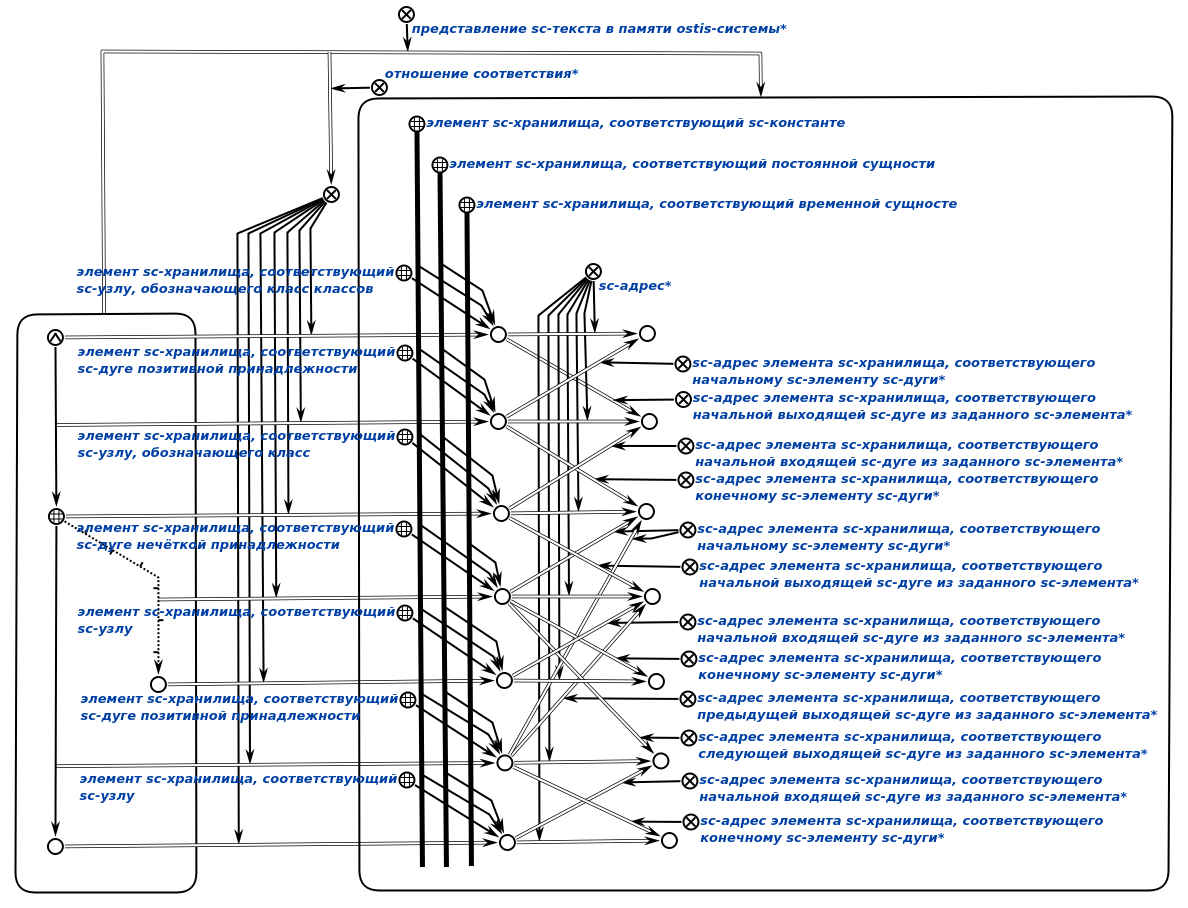
\includegraphics[scale=0.55]{author/part6/figures/sc_code_in_memory_representation.png}
	\caption{Пример спецификации представления конструкции SC-кода в памяти ostis-платформы}
	\label{fig:sc_code_in_memory_representation}
\end{figure*}

\subsection{Достоинства и недостатки Программного интерфейса Реализации sc-памяти в ostis-платформе}
\label{sec_soft_platform_sc_memory_interface_problems}

Текущий \textit{Программный интерфейс Реализации sc-памяти в ostis-платформе} позволяет:
\begin{textitemize}
	\item В необходимой и достаточной мере реализовывать платформенно-зависимые подсистемы текущего \textit{Программного варианта реализации ostis-платформы}, практически независимо от \textit{Реализации sc-памяти в ostis-платформе}. То есть текущий \textit{Программный интерфейс Реализации sc-памяти в ostis-платформе} является способом унификации доступа к программной \textit{Реализации sc-памяти в ostis-платформе} и позволяет легко подменять различные варианты реализации sc-памяти на языке представления методов С++, при этом сам \textit{Программный интерфейс Реализации sc-памяти в ostis-платформе} практически не меняется или не изменяется вовсе.
	\item Реализовывать базовые инструментальные средства для проектирования платформенно-независимых ostis-систем, например, \textit{Реализацию интерпретатор базового языка SCP}.
	\item Формировать и расширять \textit{Библиотеку многократно используемых компонентов Программного варианта реализации ostis-платформы} за счёт компонентов, использующих методы \textit{Реализации sc-памяти в ostis-платформе} и входящих в состав различных программных расширений текущего \textit{Программного интерфейса Реализации sc-памяти в ostis-платформе}.
	\item Обеспечить различные уровни доступа к \textit{Реализации sc-памяти в ostis-платформе}, в том числе уровни доступа различных пользователей \textit{Программного варианта реализации ostis-платформы}. 
\end{textitemize}

Стоит отметить, что \textit{Программный интерфейс Реализации sc-памяти в ostis-платформе} не может существовать отдельно от текущей \textit{Реализации sc-памяти в ostis-платформе}. Кроме того, он является частью \textit{Реализации sc-памяти в ostis-платформе}, то есть проектируется и разрабатывается согласованно с реализацией самой sc-памяти. Однако при необходимости он может быть использован для различных модификаций или версий текущей \textit{Реализации sc-памяти в ostis-платформе}.

Несмотря на широкий спектр функциональных возможностей текущего \textit{Программного интерфейса Реализации sc-памяти в ostis-платформе}, к его недостатком можно отнести следующее:
\begin{textitemize}
	\item На уровне \textit{Программного интерфейса Реализации sc-памяти в ostis-платформе} никак не ограничивается диапозон классов sc-элементов в sc-памяти, которые могут быть установлены в качестве аргументов, например, для \textit{Метода создания элемента в sc-памяти с заданным классом, соответствующего некоторому sc-узлу} и \textit{Метода создания элемента в sc-памяти с заданным классом, соответствующего некоторому sc-коннектору}.
	\item Из-за недостатков текущей реализации агентной архитектуры в \textit{Программном варианте реализации ostis-платформы} нельзя для \textit{Программного интерфейса Реализации sc-памяти в ostis-платформе} использовать \textit{Реализацию sc-памяти в ostis-платформе}, хранящуюся в виде скомпилированного файла. Прежде всего это связано с тем, что платформенно-зависимые агенты реализуются средствами, которые используют создание исходных файлов при сборке всей платформы. Таким образом скомпилированные файлы остаются зависимыми от того устройства, где они были собраны.
\end{textitemize}

\section{Реализация файловой памяти в Программной платформе ostis-систем}
\label{sec_soft_platform_file_memory}

\begin{SCn}

\begin{scnrelfromlist}{подраздел}
	\scnitem{\ref{sec_soft_platform_scfin_code}~\nameref{sec_soft_platform_scfin_code}}
	\scnitem{\ref{sec_soft_platform_scfin_code_alphabet_and_syntax}~\nameref{sec_soft_platform_scfin_code_alphabet_and_syntax}}
	\scnitem{\ref{sec_soft_platform_scfin_code_semantic}~\nameref{sec_soft_platform_scfin_code_semantic}}
	\scnitem{\ref{sec_soft_platform_scfin_code_example}~\nameref{sec_soft_platform_scfin_code_example}}
	\scnitem{\ref{sec_soft_platform_scfin_code_problems}~\nameref{sec_soft_platform_scfin_code_problems}}
\end{scnrelfromlist}

\begin{scnrelfromlist}{ключевой знак}
	\scnitem{Реализация файловой памяти ostis-платформы}
	\scnitem{файловая память ostis-платформы}
	\scnitem{SCfin-код}
	\begin{scnindent}
		\scnidtf{scfin-текст}
	\end{scnindent}
	\scnitem{Алфавит SCfin-кода\scnsupergroupsign}
	\scnitem{элемент файловой памяти ostis-платформы}
	\scnitem{Синтаксис SCfin-кода}
	\scnitem{Денотационная семантика SCfin-кода}
\end{scnrelfromlist}

\end{SCn}

\bigskip

\textit{SC-код} хоть и является универсальным средством для представления любых видов знаний, но не всегда есть необходимость погружать что-либо в графодинамическую память ostis-системы, по крайней мере, на ранних стадиях развития ostis-платформы. Это может быть объяснено и тем, что информационные конструкции, не принадлежащие SC-коду, достаточно сложны в понимании для неподготовленного \textit{пользователя ostis-системы}. Для решения таких проблем на уровне \textit{Алфавита SC-кода\scnsupergroupsign} вводится дополнительный элемент --- \textit{внутренний файл ostis-системы}. С помощью \textit{внутренних файлов ostis-системы} можно представлять, хранить, обрабатывать и визуализировать информационные конструкции, не принадлежащие SC-коду.

Поэтому при реализации sc-памяти необходимо учитывать необходимость хранения информационных конструкций, не принадлежащих SC-коду, с помощью SC-кода. Кроме собственно \textit{sc-памяти} \textit{Реализация sc-памяти в ostis-платформе} включает также \textit{Реализацию файловой памяти ostis-платформы}, предназначенную для хранения содержимого \textit{внутренних файлов ostis-систем}, то есть внешние информационные конструкции (линейные тексты, изображения, видео и так далее).

За весь период развития \textit{Программного варианта реализации ostis-платформы} было достаточно много попыток реализовать полно функциональное и быстрое файловую память на базе популярных баз данных. Однако из всех этих решений не было учтены потенциальные проблемы при реализации поисково-навигационной подсистемы \textit{Программного варианта реализации ostis-платформы}. Сейчас файловая память реализована своими средствами, в качестве структур данных для хранения информационных конструкций, не принадлежащих SC-коду, используются префиксные деревья \scncite{Bayer1977} и линейные списки.

Выбор аргументируется тем, что:
\begin{textitemize}
    \item префиксные структуры достаточно просты в понимании и минимальны в своём синтаксисе;
    \item с помощью префиксных структур достаточно удобно хранить и обрабатывать связи типа \scnqq{ключ-значение};
    \item доступ к значению по ключу происходит в худшем случае за длину этого ключа \scncite{Belazzougui2010};
    \item за счёт того, что префиксы склеиваются, выходит сильный выигрыш в использовании памяти.
\end{textitemize}

\begin{SCn}
\scnheader{Реализация файловой памяти ostis-платформы}
\scniselement{реализация файловой памяти на основе префиксного дерева}
\scnrelto{программная модель}{файловая память ostis-платформы}
\scniselement{многократно используемый компонент ostis-систем, хранящийся в виде файлов исходных текстов}
\scniselement{атомарный многократно используемый компонент ostis-систем}
\scniselement{зависимый многократно используемый компонент ostis-систем}
\begin{scnrelfromset}{зависимости компонента}
    \scnitem{Библиотека методов и структур данных GLib}
\end{scnrelfromset}
\begin{scnrelfromlist}{язык представления методов}
    \scnitem{C}
\end{scnrelfromlist}
\begin{scnrelfromlist}{внутренний язык}
    \scnitem{SCfin-код}
\end{scnrelfromlist}
\end{SCn}

\subsection{Формальная спецификация sc-языка внутреннего представления конструкций, не принадлежащих SC-коду, в файловой памяти ostis-платформы}
\label{sec_soft_platform_scfin_code}

Как в случае и с sc-памятью, необходимо описать sc-язык представления информационных конструкций, не принадлежащих SC-коду, внутри файловой памяти ostis-платформы. Такой sc-язык будем называть sc-языком внутреннего представления информационных конструкций, не принадлежащих SC-коду, или, кратко, \textit{SCfin-кодом (Semantic Сode file interior)}. Файловая память текстов, не принадлежащих SC-коду (как абстрактную модель, по которой можно реализовывать соответствующее ей файловую память ostis-платформы), можно рассматривать как подмножество scfin-текста.

\begin{SCn}
\scnheader{SCfin-код}
\scnidtf{Semantic Code file interior}
\scnidtf{Sc-язык внутренного смыслового представления информационных конструкций, не принадлежащих SC-коду, внутри файловой памяти ostis-платформы}
\scnidtf{метаязык описания представления информационных конструкций, не принадлежащих SC-коду, внутри файловой памяти ostis-платформы}
\scntext{часто используемый неосновной внешний идентификатор sc-элемента}{scfin-текст}
\begin{scnindent}
    \scniselement{имя нарицательное}
\end{scnindent}
\scniselement{абстрактный язык}
\scniselement{метаязык}
\scniselement{sc-язык}
\scnsubset{SC-код}
\scnsuperset{файловая память ostis-платформы}
\end{SCn}

\subsection{Синтаксис SCfin-кода}
\label{sec_soft_platform_scfin_code_alphabet_and_syntax}

\textit{Синтаксис SCfin-кода} задается: (1) \textit{Алфавитом SCfin-кода}, (2) отношением порядка \textit{последовательность в линейном тексте*}.

\begin{SCn}
\scnheader{Алфавит SCfin-кода\scnsupergroupsign}
\scnidtf{синтаксический тип элемента файловой памяти ostis-платформы}
\scnidtf{Множество типов элементов файловой памяти ostis-платформы}
\scnrelto{алфавит}{SCfin-код}
\begin{scneqtoset}
    \scnitem{элемент файловой памяти ostis-платформы, соответствующий подстроке текста линейного языка}
\end{scneqtoset}
\end{SCn}

\textit{Алфавит SCfin-кода\scnsupergroupsign} состоит из одного синтаксически выделяемого типа элементов файловой памяти --- \textit{элемента файловой памяти ostis-платформы, соответствующего подстроке текста линейного языка}.

\begin{SCn}
\scnheader{элемент файловой памяти ostis-платформы, соответствующий подстроке текста линейного языка}
\scniselement{sc-элемент}
\scnidtf{элемент файловой памяти ostis-платформы}
\scnidtf{ячейка файловой памяти ostis-платформы}
\scnidtf{образ подстроки информационной конструкции, не принадлежащей SC-коду, в рамках файловой памяти ostis-платформы}
\end{SCn}

Отношение \textit{последовательности в линейном тексте*} определяется как бинарное ориентированное отношение порядка, компонентами каждой ориентированной пары которого является элементы файловой памяти ostis-платформы, соответствующие некоторым подстрокам линейного текста, в результате конкатенации которых образуется подстрока, принадлежащая этому же линейному тексту.

\textit{Синтаксис SCfin-кода} достаточно прост, поскольку информационные конструкции на нём задаются при помощи \textit{Алфавита SCfin-кода}, мощность которого равна 1, и единственного отношения инцидентности \textit{последовательности в линейном тексте*}. Иерархии синтаксических элементов как таковые не выделяются, поскольку в этом нет необходимости.

На уровне реализации важно выделить семантические классы \textit{элементов файловой памяти ostis-платформы, соответствующий подстроке текста линейного языка}, которые обозначают некоторую префиксную или постфиксную часть целой информационной конструкции.

\subsection{Денотационная семантика SCfin-кода}
\label{sec_soft_platform_scfin_code_semantic}

\begin{SCn}
\scnstructheader{Семантическая классификация элементов SCfin-кода}
\begin{scnsubstruct}

\scnheader{элемент файловой памяти ostis-платформы, соответствующий текста линейного языка}
\scnrelfrom{разбиение}{Типология элементов по месту расположения подстроки в линейном тексте}
\begin{scnindent}
    \begin{scneqtoset}
        \scnitem{элемент файловой памяти ostis-платформы, соответствующий префиксной подстроке текста линейного языка}
        \scnitem{элемент файловой памяти ostis-платформы, соответствующий постфиксной подстроке текста линейного языка}
    \end{scneqtoset}
\end{scnindent}

\end{scnsubstruct}
\end{SCn}

На SCfin-коде достаточно просто задавать информационные конструкции любых линейных текстов. Однако с точки зрения реализуемой модели sc-памяти есть необходимость задавать не столько форму информационных конструкций, не принадлежащих SC-коду, внутри файловой памяти ostis-платформы, сколько связи между этими внещними информационными конструкциями файлами ostis-системы, являющихся знаками SC-кода. Одновременно должны быть реализованы на уровне sc-памяти и метод получения файлов ostis-системы, которые содержат заданную внешнюю информационную конструкцию, и методы получения внешних информационных конструкций из заданных файлов ostis-системы.

\subsection{Описание процесса и пример трансляции внешних информационных конструкций в файловую память ostis-платформы}
\label{sec_soft_platform_scfin_code_example}

На рисунке \nameref{fig:file_in_memory_representation} показано представление информационных конструкций, не принадлежащих SC-коду и соответствия между файлами ostis-системы и информационными конструкциями. С помощью отношения \textit{множество sc-адресов файлов ostis-системы по префиксам их содержимого*} задаётся бинарная ориентированная пара, первым компонентом которой является префиксная структура, элементами которой являются подстроки внешних информационных конструкций, а вторым компонентом --- множество соотвествующих им sc-адресов файлов ostis-системы, а с помощью отношения \textit{множество постфиксов содержимого файлов ostis-системы по их sc-адресам*} задаётся бинарная ориентированная пара, первым компонентом которой является префиксная структура, элементами которой являются подстроки sc-адресов файлов ostis-системы, представленных в строковом виде, а вторым компонентом --- множество соотвествующих им постфиксов внешних информационных конструкций префиксной структуры, являющейся первым компонентом каждой пары отношения \textit{множество sc-адресов файлов ostis-системы по префиксам их содержимого*}.

\begin{figure*}[htbp]
	\center
	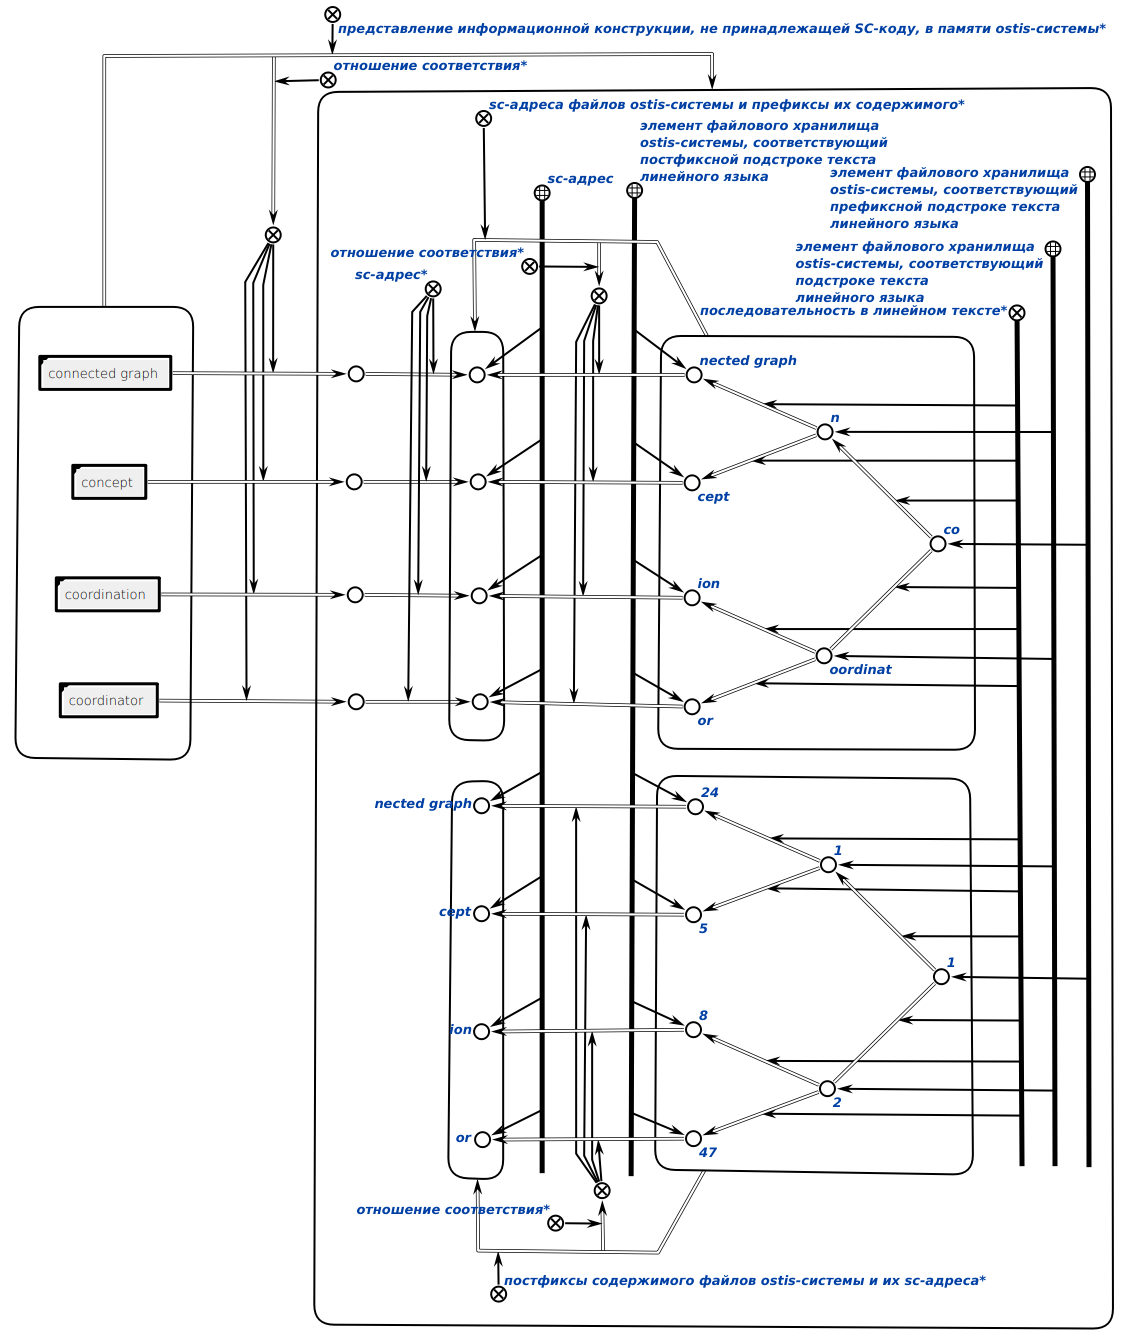
\includegraphics[scale=0.6]{author/part6/figures/file_in_memory_representation.png}
	\caption{Пример спецификации представления информационных конструкций, не принадлежащих SC-коду, в памяти ostis-системы}
	\label{fig:file_in_memory_representation}
\end{figure*}

\subsection{Достоинства и недостатки Реализации файловой памяти ostis-платформы и sc-языка внутреннего представления внешних информационных конструкций в файловой памяти ostis-платформы}
\label{sec_soft_platform_scfin_code_problems}

Используемая \textit{Реализация файловой памяти ostis-платформы} полностью оправдывает себя при взаимодействии с системой. Благодаря использованию префиксных структур асимптотические сложности метода получения множества внешних информационных конструкций из заданных файлов ostis-системы и метода получения множества файлов ostis-системы по заданным внешним информационным конструкциям линейны, так как зависит от длины заданной строки и структуры префиксного дерева.

Среди общих недостатков данной \textit{Реализации файловой памяти ostis-платформы} можно выделить следующие:
\begin{textitemize}
    \item Информационные конструкции, не принадлежащие SC-коду, пока полностью хранятся в оперативной памяти компьютерного устройства, на котором развёрнута платформа. Данную проблему можно решить, если в оперативной памяти хранить только первые знаки подстрок информационных конструкций, а остальные части этих подстрок хранить на уровне файлового системы.
    \item На данный момент информационно-поисковая подсистема реализована не полностью. \textit{Реализация файловой памяти ostis-платформы} позволяет быстро решать задачи поиска внешних информационных конструкций по их префиксным подстрокам, однако не позволяет быстро решать задачи поиска информационных конструкций по любой подстроке, даже для которого задан некоторый шаблон-образец.
\end{textitemize}

Описанные проблемы будут решены в рамках будущей версии \textit{Программного варианта реализации ostis-платформы}.

\section{Реализация подсистемы взаимодействия c sc-памятью на основе языка JSON}
\label{sec_soft_platform_sc_server_subsystem}

\begin{SCn}

\begin{scnrelfromlist}{подраздел}
	\scnitem{\ref{sec_soft_platform_sc_json_code}~\nameref{sec_soft_platform_sc_json_code}}
	\scnitem{\ref{sec_soft_platform_sc_json_code_alphabet_and_syntax}~\nameref{sec_soft_platform_sc_json_code_alphabet_and_syntax}}
	\scnitem{\ref{sec_soft_platform_sc_json_code_grammar}~\nameref{sec_soft_platform_sc_json_code_grammar}}
	\scnitem{\ref{sec_soft_platform_sc_server}~\nameref{sec_soft_platform_sc_server}}
\end{scnrelfromlist}

\begin{scnrelfromlist}{ключевой знак}
	\scnitem{Реализация подсистемы взаимодействия c sc-памятью на основе языка JSON}
	\scnitem{Серверная система на основе Websocket и JSON, обеспечивающая сетевой доступ к sc-памяти}
	\scnitem{Реализация клиентской системы на языке программирования Python}
	\scnitem{Реализация клиентской системы на языке программирования TypeScript}		
	\scnitem{Реализация клиентской системы на языке программирования C\#}
	\scnitem{Реализация клиентской системы на языке программирования Java}
	\scnitem{SC-JSON-код}
	\scnitem{команда на SC-JSON-коде}
	\scnitem{ответ на команду на SC-JSON-коде}
\end{scnrelfromlist}

\end{SCn}

\bigskip

В общем случае подсистема взаимодействия ostis-платформы с внешней средой может быть реализована по-разному. Так, например, до момента реализации текущей подсистемы ранее существовал её аналог на языке программирования Python, который использовал протокол HTTP и бинарное представление команд и ответов.
Поэтому можно говорить о большом разнообразии таких подсистем, которые будут составлять множество всевозможных \textit{Реализаций подсистемы взаимодействия с внешней средой с использованием сетевых языков}.

Данная \textit{Реализация подсистемы взаимодействия c sc-памятью на основе языка JSON} позволяет ostis-системам взаимодействовать с системами из внешней среды на основе общепринятого транспортного формата передачи данных JSON и предоставляет API для доступа к sc-памяти платформы интерпретации sc-моделей.

\begin{SCn}
\scnheader{Реализация подсистемы взаимодействия с внешней средой с использованием сетевых языков}
\begin{scnrelfromset}{декомпозиция программной системы}
    \scnitem{Реализация подсистемы взаимодействия с внешней средой с использованием сетевых языков на основе языка JSON}
\end{scnrelfromset}
\end{SCn}

\begin{SCn}
\scnheader{Реализация подсистемы взаимодействия c sc-памятью на основе языка JSON}
\scnidtf{Подсистема взаимодействия с sc-памятью на основе формата JSON}
\scniselement{многократно используемый компонент ostis-систем, хранящийся в виде файлов исходных текстов}
\scniselement{неатомарный многократно используемый компонент ostis-систем}
\scniselement{зависимый многократно используемый компонент ostis-систем}
\scniselement{клиент-серверная система}
\begin{scnrelfromlist}{используемый язык представления методов}
    \scnitem{C}
    \scnitem{C++}
    \scnitem{Python}
    \scnitem{TypeScript}
    \scnitem{C\#}
    \scnitem{Java}
\end{scnrelfromlist}
\begin{scnrelfromlist}{используемый язык}
    \scnitem{SC-JSON-код}
\end{scnrelfromlist}
\begin{scnrelfromset}{декомпозиция программной системы}
    \scnitem{Серверная система на основе Websocket и JSON, обеспечивающая сетевой доступ к sc-памяти}
    \scnnonamednode
    \begin{scneqtoset}
        \scnitem{Реализация клиентской системы на языке программирования Python}
        \scnitem{Реализация клиентской системы на языке программирования TypeScript}
        \scnitem{Реализация клиентской системы на языке программирования C\#}
        \scnitem{Реализация клиентской системы на языке программирования Java}
    \end{scneqtoset}
\end{scnrelfromset}
\end{SCn}

Взаимодействие c sc-памятью обеспечивается с помощью передачи информации на \textit{SC-JSON-коде} и ведётся, с одной стороны, между сервером, являющегося частью ostis-системы, написанным на том же языке реализации этой ostis-системы и имеющим доступ к её sc-памяти, и с другой стороны множеством клиентоd, которым известно о наличии сервера в пределах сети их использования. С помощью подсистемы взаимодействия с sc-памятью на основе языка JSON можно взаимодействовать с ostis-системой на таком же множестве возможных операций, как и в случае, если бы взаимодействие происходило (непосредственно) напрямую, на том же языке реализации платформы интерпретации sc-моделей компьютерных систем. При этом результат работы отличается только скоростью обработки информации.
Взаимодействие программной модели sc-памяти с внешними ресурсами может осуществляться посредством специализированного программного интерфейса (API), однако этот вариант неудобен в большинстве случае, поскольку:
    \begin{textitemize}
        \item поддерживается только для очень ограниченного набора языков программирования;
        \item требует того, чтобы клиентское приложение, обращающееся к программной модели sc-памяти, фактически составляло с ней единое целое, таким образом исключается возможность построения распределенного коллектива ostis-систем;
        \item как следствие предыдущего пункта, исключается возможность параллельной работы с sc-памятью нескольких клиентских приложений.
   \end{textitemize}
Для того, чтобы обеспечить возможность удаленного доступа к sc-памяти не учитывая при этом языки программирования, с помощью которых реализовано конкретное клиентское приложение, было принято решение о реализации возможности доступа к sc-памяти с использованием универсального языка, не зависящего от средств реализации того или иного компонента или системы.

Среди эффективных протоколов, используемых при реализации клиент-серверных систем, стоит отметить протоколы прикладного уровня стека TCP/IP --- протоколы HTTP и WebSocket \scncite{Bhumij2018}. Целесообразным является использование протокола WebSocket, это объясняется следующими причинами:

\begin{textitemize}
    \item WebSocket выгодно использовать в веб-ориентированных системах, в которых данные, отправляемые сервером, представляются или сохраняются на стороне клиента. В WebSocket данные постоянно передаются через одно и то же открытое соединение, поэтому коммуникация по протоколу WebSocket быстрее чем коммуникация по HTTP \scncite{Tomasetti2021}, \scncite{Bhumij2018}. Это очень важно с точки зрения проектирования Экосистемы OSTIS, которые могут состоять из десятков тысяч различного вида ostis-систем.
    \item Поскольку в основе ostis-систем лежит идея агентно-ориентированной обработки знаний (асинхронной обработки), а память таких систем должна быть одновременно распределённой и общей, то необходимо, чтобы каждая из них (в частности, самостоятельная ostis-система) могла общаться с другими ostis-системами. Причём такое общение может и должно происходить на условиях инициирования событий в памяти этих систем. Отсюда следует однозначный вывод, что протокол HTTP не может быть использован в передовых интеллектуальных системах нового поколения по причине однонаправленности создаваемого им соединения.
\end{textitemize}
В качестве языка коммуникации систем был разработан строковый язык на базе языка JSON \scncite{Marrs2017} --- SC-JSON-код. Его выбор объясняется гибкостью задания отношений между описываемыми им объектами.

\subsection{Формальная спецификация sc-языка представления сообщений между подсистемами Программного варианта реализации ostis-платформы. SC-JSON-код}
\label{sec_soft_platform_sc_json_code}

Как говорилось ранее, подсистемы в рамках реализуемого программного варианта специализированной платформы общаются с помощью языка внешнего представления знаний SC-JSON-код. Данный язык является строковым, то есть линейным, и легкообратаваемым, поскольку существует большое количество средств для обработки его надъязыка JSON.

\begin{SCn}
\scnheader{SC-JSON-код}
\scnidtf{Semantic JSON-code}
\scnidtf{Semantic JavaScript Object Notation code}
\scnidtf{Язык внешнего смыслового представления знаний на основе языка JSON}
\scntext{часто используемый неосновной внешний идентификатор sc-элемента}{sc-json-текст}
\begin{scnindent}
    \scniselement{имя нарицательное}
\end{scnindent}
\scniselement{абстрактный язык}
\scniselement{линейный язык}
\scnsubset{JSON}
\end{SCn}

\subsection{Синтаксис SC-JSON-кода}
\label{sec_soft_platform_sc_json_code_alphabet_and_syntax}

\textit{Синтаксис SC-JSON-кода} задается: (1) \textit{Алфавитом SC-JSON-кода}, (2) Грамматикой SC-JSON-кода. В алфавите SC-JSON-кода выделяется базовая синтаксическая классификация его элементов.

\begin{SCn}
\scnstructheader{Синтаксическая классификация элементов SC-JSON-кода}

\begin{scnsubstruct}
\scnstructheader{SC-JSON-код}
\scnrelto{семейство подмножеств}{sc-json-предложение}
\begin{scnindent}
    \scnsubset{json-список json-пар}
    \scnrelto{семейство подмножеств}{sc-json-пара*}
    \begin{scnindent}
        \begin{scnreltovector}{декартово произведение}
            \scnitem{sc-json-строка}
            \scnitem{sc-json-объект}
        \end{scnreltovector}
    \end{scnindent}
    \begin{scnrelfromset}{разбиение}
        \scnitem{команда на SC-JSON-коде}
        \scnitem{ответ на команду на SC-JSON-коде}
    \end{scnrelfromset}
\end{scnindent}

\scnheader{sc-json-объект}
\begin{scnrelfromset}{разбиение}
    \scnitem{sc-json-cписок}
    \scnitem{sc-json-пара}
    \scnitem{sc-json-литерал}
    \begin{scnindent}
        \begin{scnrelfromset}{разбиение}
            \scnitem{sc-json-строка}
            \scnitem{sc-json-число}
        \end{scnrelfromset}
    \end{scnindent}
\end{scnrelfromset}
\end{scnsubstruct}
\end{SCn}

\textit{Алфавит SC-JSON-кода\scnsupergroupsign} представляет собой множество всех возможных символов в SC-JSON-коде. Поскольку \textit{SC-JSON-код} является линейным строковым языком представления знаний, то его алфавит включает объединение алфавитов всех языков, тексты на которых могут представлять внешние идентификаторы и/или содержимое файлов ostis-системы, множество всех цифр и множество всех других специальных символов. Последовательности знаков алфавита могут образовывать sc-json ключевые слова, \textit{sc-json-пары}, \textit{sc-json-предложения} из \textit{sc-json-пар} и \textit{sc-json-тексты} из \textit{sc-json-предложений}. При этом конструкции на SC-JSON-коде строятся по следующим синтаксическим правилам:
\begin{textitemize}
    \item Каждое правило \textit{Грамматики SC-JSON-кода} описывает корректный с точки зрения \textit{Синтаксиса SC-JSON-кода} порядок sc-json-объектов в sc-json-предложении. Совокупность правил \textit{Грамматики SC-JSON-кода} описывает корректный с точки зрения \textit{Синтаксиса SC-JSON-кода} порядок sc-json-предложений в sc-json-тексте. Каждое sc-json-предложение является sc-json-списком, состоящим из sc-json-пар и представляет собой команду или ответ на эту команду.
    \item Каждая \textit{команда (ответ на команду) на SC-JSON-коде} состоит из заголовка, включающего sc-json-пары описания самой команды (ответа на команду), и сообщения, различного для каждого класса команд (ответов на команды). Сообщение \textit{команды (ответа на команду) на SC-JSON-коде} обычно представляет собой список sc-json-объектов и может не ограничиваться по мощности.
    \item Каждая sc-json-пара состоит из двух элементов: ключевого слова и некоторого другого sc-json-объекта, ассоциируемого с этим ключевым словом. Набор ключевых слов в sc-json-парах определяется конкретным классом \textit{команд (ответов на команды) на SC-JSON-коде}. Sc-json-пара начинается знаком открывающейся фигурной скобки \scnqq{\{} и заканчивается знаком закрывающейся фигурной скобки \scnqq{\}}. Ключевое слово и sc-json-объект, ассоциируемый с ним, разделяются при помощи знака двоеточия \scnqq{:}.
    \item Sc-json-строки, записанные в sc-json-текстах, начинаются и заканчиваются знаком двух ковычек \textquotedblleft.
    \item Sc-json-списки, состоящие не из sc-json-пар, начинаются знаком открывающейся квадратной скобки \scnqq{[} и заканчиваются знаком закрывающейся квадратной скобки \scnqq{]}. Sc-json-объекты в sc-json-списках разделяются запятыми \scnqq{,}.
\end{textitemize}

\subsection{Грамматика SC-JSON-кода}
\label{sec_soft_platform_sc_json_code_grammar}

Грамматика SC-JSON-кода представляет собой множество всех возможных правил, используемых при построении команд и ответов на них на SC-JSON-коде. Каждой команде \textit{SC-JSON-кода} однозначно соответствует правило грамматики \textit{SC-JSON-кода}. Правила \textit{Грамматики SC-JSON-кода} позволяют правильно представлять команды на SC-JSON-коде. Каждое правило грамматики \textit{SC-JSON-кода} представляется в виде правила на \textit{Языке описания грамматик ANTLR} и его интерпретации на естественном языке.

\begin{SCn}
\scnheader{Грамматика SC-JSON-кода}
\scnhaselementrole{ключевой sc-элемент}{Правило, задающее синтаксис \textit{команд на SC-JSON-коде}}
\begin{scnindent}
    \scnrelto{синтаксическое правило}{команда на SC-JSON-коде}
\end{scnindent}
\scnhaselementrole{ключевой sc-элемент}{Правило, задающее синтаксис \textit{ответов на команды на SC-JSON-коде}}
\begin{scnindent}
    \scnrelto{синтаксическое правило}{ответ на команду на SC-JSON-коде}
\end{scnindent}
\scnhaselement{Правило, задающее синтаксис \textit{команды создания sc-элементов}}
\begin{scnindent}
    \scnrelto{синтаксическое правило}{команда создания sc-элементов}
\end{scnindent}
\scnhaselement{Правило, задающее синтаксис \textit{ответа на команду создания sc-элементов}}
\begin{scnindent}
    \scnrelto{синтаксическое правило}{ответ на команду создания sc-элементов}
\end{scnindent}
\end{SCn}

Правило, задающее синтаксис \textit{команд на SC-JSON-коде} представлено на рисунке \nameref{fig:command}. Класс \textit{команд на SC-JSON-коде} включает \textit{команду создания sc-элементов}, \textit{команду получения соответствующих типов sc-элементов}, \textit{команду удаления sc-элементов}, \textit{команду обработки ключевых sc-элементов}, \textit{команду обработки содержимого файлов ostis-системы}, \textit{команду поиска sc-конструкций, изоморфных заданному sc-шаблону}, \textit{команду генерации sc-конструкции, изоморфной заданному sc-шаблону}, и \textit{команду обработки sc-событий}. В \textit{команду на SC-JSON-коде} включаются идентификатор этой команды, тип и сообщение.

\begin{figure}[htbp]
  \center
  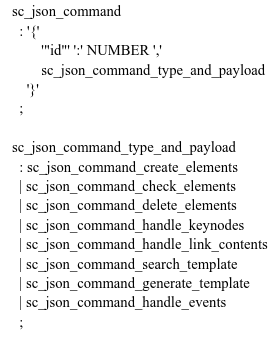
\includegraphics[scale=0.9]{author/part6/figures/command.png}
  \caption{Описание Правила, задающего синтаксис \textit{команд на SC-JSON-коде}}
  \label{fig:command}
\end{figure}

Правило, задающее синтаксис \textit{ответа на команду на SC-JSON-коде} описывает синтаксис ответов на команды, описываемых предыдущим правилом. Класс \textit{ответов на команды на SC-JSON-коде} включает \textit{ответ на команду создания sc-элементов}, \textit{ответ на команду получения соответствующих типов sc-элементов}, \textit{ответ на команду удаления sc-элементов}, \textit{ответ на команду обработки ключевых sc-элементов}, \textit{ответ на команду обработки содержимого файлов ostis-системы}, \textit{ответ на команду поиска sc-конструкций, изоморфных заданному sc-шаблону}, \textit{ответ на команду генерации sc-конструкции, изоморфной заданному sc-шаблону}, и \textit{ответ на команду обработки sc-событий}. В \textit{ответ на команду на SC-JSON-коде} включаются идентификатор соответствующей команды, статус обработки ответа и ответное сообщение \nameref{fig:command_answer}.

\begin{figure}[htbp]
  \center
  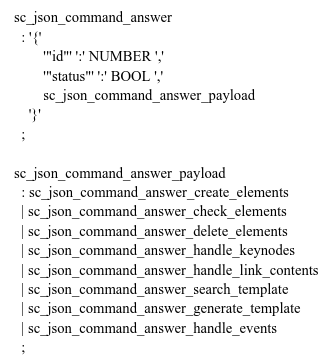
\includegraphics[scale=0.8]{author/part6/figures/command_answer.png}
  \caption{Описание Правила, задающего синтаксис \textit{ответов на команды SC-JSON-кода}}
  \label{fig:command_answer}
\end{figure}

В сообщении \textit{команды создания sc-элементов} представляется список описаний создаваемых sc-элементов. Такими sc-элементами могут быть sc-узел, sc-дуга, sc-ребро или файл ostis-системы. Тип sc-элемента указывается в паре с ключевым словом \scnqq{el}: для sc-узла sc-json-тип элемента представляется как \scnqq{node}, для sc-дуги и sc-ребра --- \scnqq{edge}, для файла ostis-системы --- \scnqq{link}. Метки типов sc-элементов уточняются в соответствующих им описаниях в сообщении команды в паре с ключевым словом \scnqq{type}. Если создаваемым sc-элементом является файл ostis-системы, то дополнительно указывается содержимое этого файла ostis-системы в паре с ключевым словом \scnqq{content}, если создаваемым sc-элементом является sc-дуга или sc-ребро, то указываются описания sc-элементов, из которых они выходят, и sc-элементов, в которые они входят. Описание таких sc-элементов состоят из двух пар: первая пара указывает на способ ассоциации с sc-элементом и представляется как \scnqq{addr} или \scnqq{idtf} или \scnqq{ref} в паре с ключевым словом \scnqq{type}, вторая пара --- то, по чему происходит ассоциация с этим sc-элементом: его хэшу, системному идентификатору или номеру в массиве создаваемых sc-элементов --- в паре с ключевым словом \scnqq{value} \nameref{fig:create_elements_command}.

\begin{figure}[htbp]
	\center
	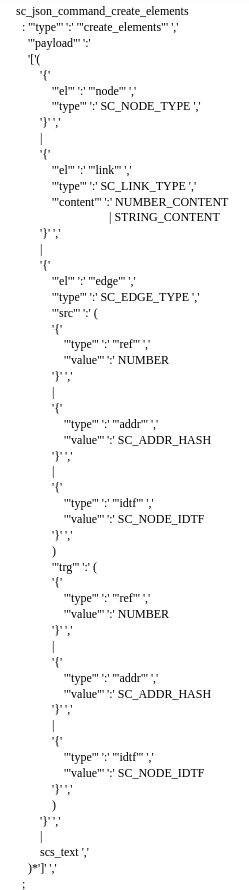
\includegraphics[scale=0.8]{author/part6/figures/create_elements_command.png}
	\caption{Описание Правила, задающего синтаксис \textit{команды создания sc-элементов}}
	\label{fig:create_elements_command}
\end{figure}

Сообщением \textit{ответа на команду создания sc-элементов} является список хэшей созданных sc-элементов, соответствующих описаниям \textit{команды создания sc-элементов} со статусом 1, в случае успешной обработки команды \nameref{fig:create_elements_command_answer}.

\begin{figure}[htbp]
	\center
	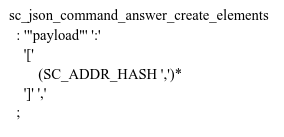
\includegraphics[scale=0.8]{author/part6/figures/create_elements_command_answer.png}
	\caption{Описание Правила, задающего синтаксис \textit{ответа на команду создания sc-элементов}}
	\label{fig:create_elements_command_answer}
\end{figure}

Множество \textit{команд на SC-JSON-коде} легко расширяемо засчёт гибкости и функциональности языка JSON. Множество \textit{ответов на команды на SC-JSON-коде} также легко расширяемо вместе с расширением \textit{команд на SC-JSON-коде}.

Детальное описание синтаксиса команд и ответов на эти команды, а также их примеры можно найти в Стандарте OSTIS (см. \scncite{Standart2021}).

\subsection{Реализация Серверной системы на основе Websocket и JSON, обеспечивающей сетевой доступ к sc-памяти}
\label{sec_soft_platform_sc_server}

\textit{Реализация Серверной системы на основе Websocket и JSON, обеспечивающей сетевой доступ к sc-памяти}, представляет собой интерпретатор команд и ответов на них \textit{SC-JSON-кода} на программное представление sc-конструкций в sc-памяти при помощи \textit{Библиотеки программных компонентов для обработки json-текстов JSON for Modern C++} и \textit{Библиотеки кросс-платформенных программных компонентов для реализации серверных приложений на основе Websocket WebSocket++}, а также обеспечивается комплексным тестовым покрытием посредством программных фреймворков Google Tests и Google Benchmark Tests. \textit{Библиотека программных компонентов для обработки json-текстов JSON for Modern C++} имеет богатый, удобный и быстродействующий функционал, необходимый для реализации подобных компонентов ostis-систем, а \textit{Библиотека кросс-платформенных программных компонентов для реализации серверных приложений на основе Websocket WebSocket++} позволяет элегантно проектировать серверные системы без использовании избыточных зависимостей и решений. Настройка программного компонента осуществляется с помощью \textit{Программного компонента настройки программных компонентов ostis-систем} и скриптов языков CMake и Bash.

\begin{SCn}
\scnheader{Реализация Серверной системы на основе Websocket и JSON, обеспечивающей сетевой доступ к sc-памяти}
\scnidtf{Реализация системы, работающей по принципам Websocket и предоставляющая параллельно-асинхронный многоклиентский доступ к sc-памяти платформы интерпретации sc-моделей при помощи SC-JSON-кода}
\scnidtf{sc-json-сервер}
\scntext{часто используемый неосновной внешний идентификатор sc-элемента}{sc-сервер}
\scniselement{многократно используемый компонент ostis-систем, хранящийся в виде файлов исходных текстов}
\scniselement{атомарный многократно используемый компонент ostis-систем}
\scniselement{зависимый многократно используемый компонент ostis-систем}
\begin{scnrelfromlist}{используемый язык представления методов}
    \scnitem{C}
    \scnitem{C++}
\end{scnrelfromlist}
\begin{scnrelfromlist}{используемый язык}
    \scnitem{SC-JSON-код}
\end{scnrelfromlist}
\begin{scnrelfromset}{зависимости компонента}
    \scnitem{Библиотека программных компонентов для обработки json-текстов JSON for Modern C++}
    \scnitem{Библиотека кросс-платформенных программных компонентов для реализации серверных приложений на основе Websocket WebSocket++}
    \scnitem{Программный компонент настройки программных компонентов ostis-систем версия}
    \scnitem{Реализация sc-памяти}
\end{scnrelfromset}
\end{SCn}

Стоит отметить, что текущая \textit{Реализация Cерверной системы на основе Websocket и JSON, обеспечивающей сетевой доступ к sc-памяти}, не является первой в своём роде и заменяет предыдущую ее реализацию, написанную на языке Python. Причина такой замены состоит в следующем:
\begin{textitemize}
    \item предыдущая \textit{Реализация Cерверной системы на основе Websocket, обеспечивающей доступ к sc-памяти при помощи команд SC-JSON-кода}, реализованная на языке программирования Python, зависит от библиотеки Boost Python, предоставляемой сообществом по развитию и коллаборации языков С++ и Python. Дело в том, что такое решение требует поддержки механизма интерпретации программного кода на языке Python на язык С++, что является избыточным и необоснованным, поскольку большая часть программного кода \textit{Программного варианта реализации ostis-платформы} реализована на языках С и С++. Новая реализация описываемой программной системы позволяет избавиться от использования ёмких и ресурсозатратных библиотек(например, boost-python-lib, llvm) и языка Python;
    \item при реализации распределённых подсистем важную роль играет скорость обработки знаний, то есть возможность быстро и своевременно отвечать на запросы пользователя. Качество доступа к sc-памяти посредством реализованной \textit{Подсистемы взаимодействия с sc-памятью на основе языка JSON} должно быть соизмеримо с качеством доступа к sc-памяти при помощи специализированного программного интерфейса API, реализованного на том же языке программирования, что и сама система. Новая реализация позволяет повысить скорость обработки запросов \textit{Подсистемой взаимодействия с sc-памятью на основе языка JSON}, в том числе и обработка знаний, не менее чем в 1,5 раза по сравнению с предыдущим вариантом реализации этой подсистемы.
\end{textitemize}

\textit{Реализация Серверной системы на основе Websocket и JSON, обеспечивающей сетевой доступ к sc-памяти}, обладает следующими общими характеристиками:
\begin{textitemize}
    \item Cерверная подсистема имеет такой же специализированный программный интерфейс, как и \textit{Реализация sc-памяти}, однако взаимодействие с ней при помощи такого интерфейса осуществляется посредством сети. Это обеспечивает возможность взаимодействия клиентских систем, реализованных на разных языкаъ программирования, с одной общей памятью.
    \item Данную подсистему можно рассматривать как некоторый интерпретатор внешнего языка представления знаний SC-JSON-код, на котором могут общаться ostis-системы, реализованные на базе специализированной ostis-платформы. Каждой команде и ответу на команду этого языка соответствует обработчик (потенциально и вовсе агент), который является частью этого интерпретатора. Сам язык внешнего представления знаний SC-JSON-код независим от реализации платформы и используется только как язык внешнего представления знаний, но может быть задействован при реализации других средств и интерпретаторов sc-моделей ostis-систем.
    \item Реализованный программный компонент предоставляет многопользовательский асинхронный доступ к sc-памяти. В ходе тестирования sc-сервера выяснилось, что его реализация позволяет обрабатывать запросы не менее чем 1000 клиентских систем. В связи с необходимостью обеспечения параллельного доступа к sc-памяти на уровне реализации программного компонента были добавлены блоки синхронизации. Например, в реализации можно заметить очередь команд на обработку системой --- вне зависимости от количества клиентских систем и того, в каком количестве они отправляют команды на обработку, все команды могут становиться в очередь. Такое решение позволяет временно обойти проблемы взаимодействия блоков синхронизации на уровне sc-памяти при обработки разных типов команд над ней (поисковых, генеративных, деструктивных и так далее). При этом серверную систему невозможно отключить до тех пор, пока очередь команд имеет какие-нибудь необработанные команды. Также серверная система продолжает работать, если в списке идентификаторов клиентских систем остались неотключенные из них. Необходимость данных функций серверной подсистемы обуславливается необходимостью поддержки атомарности запросов, обрабатываемых системой.
    \item В процессе тестирования подсистемы были получена оценка её скорости обработки команд и ответов. При нагрузочном тестировании использовалась тестовая клиентская система, написанная на С++ и не имеющая функционала обработки текстов SC-JSON-кода. В результате тестирования было выяснено, что при отправке 1000 различных команд: команд создания sc-элементов, команд обработки содержимого файлов ostis-системы и команд удаления sc-элементов --- время, потраченное на их обработку не превышало 0,2 секунды. При этом в отдельных случаях на обработку 1000 команд создания sc-элементов уходило не более 0,14 секунды, команд удаления sc-элементов --- не более 0,07 секунды, команд обработки содержимого файлов ostis-системы --- не более 0,27 секунды, команд поиска sc-конструкций, изоморфных заданному sc-шаблону --- не более 0,45 секунды.
\end{textitemize}

\textit{Реализация Серверной системы на основе Websocket и JSON, обеспечивающей сетевой доступ к sc-памяти} обеспечивает необходимый и достаточный программный интерфейс для взаимодействия c sc-памятью. В общем случае описывает функциональные возможности не только \textit{Серверной системы на основе Websocket, обеспечивающей доступ к sc-памяти платформы интерпретации sc-моделей при помощи команд SC-JSON-кода}, но и клиентских систем взаимодействующих с ней, поскольку зачастую эти клиентские системы включают специализированный программный интерфейс, схожий с интерфейсом серверной системы, но реализованный на другом языке представления методов (языке программирования).

\section{Реализация интерпретатора sc-моделей пользовательских интерфейсов}
\label{sec_soft_platform_sci_machine}

\begin{SCn}

\begin{scnrelfromlist}{подраздел}
	\scnitem{\ref{sec_soft_platform_sci_machine_components}~\nameref{sec_soft_platform_sci_machine_components}}
	\scnitem{\ref{sec_soft_platform_sci_machine_problems}~\nameref{sec_soft_platform_sci_machine_problems}}
\end{scnrelfromlist}

\end{SCn}

В большинстве случаев разработка пользовательского интерфейса в современных системах отнимает большую часть времени, затрачиваемого на разработку всей системы. Однако эффективность использования программной системы зависит от разрабатываемого пользовательского интерфейса \scncite{Myers1992}.

Наряду с \textit{Реализацией sc-памяти} важной частью \textit{Программного варианта реализации ostis-платформы} является \textit{Реализация интерпретатора sc-моделей пользовательских интерфейсов}, которая предоставляет базовые средства просмотра и редактирования базы знаний пользователем, средства для навигации по базе знаний (задания вопросов к базе знаний) и может дополняться новыми компонентами в зависимости от задач, решаемых каждой конкретной ostis-системой.

\begin{SCn}
	\scnheader{Реализация интерпретатора sc-моделей пользовательских интерфейсов}
	\scniselement{многократно используемый компонент ostis-систем, хранящийся в виде файлов исходных текстов}
	\scniselement{неатомарный многократно используемый компонент ostis-систем}
	\scniselement{зависимый многократно используемый компонент ostis-систем}
	\begin{scnrelfromlist}{используемый язык представления методов}
		\scnitem{JavaScript}
		\scnitem{TypeScript}
		\scnitem{Python}
		\scnitem{HTML}
		\scnitem{CSS}
	\end{scnrelfromlist}
	\begin{scnrelfromset}{зависимости компонента}
		\scnitem{Библиотека стандартных интерфейсных компонентов на языке программирования JavaScript}
		\scnitem{Библиотека для реализации серверных приложений на языке программирования Python Tornado}
		\scnitem{Реализация клиентской системы на языке программирования TypeScript}
		\scnitem{Реализация клиентской системы на языке программирования Python}
	\end{scnrelfromset}
\end{SCn}

Важным принципом \textit{Реализации интерпретатора sc-моделей пользовательских интерфейсов} является простота и однотипность подключения любых компонентов пользовательского интерфейса (редакторов, визуализаторов, переключателей, команд меню и так далее). Для этого реализуется программная прослойка Sandbox, в рамках которой реализуются низкоуровневые операции взаимодействия с серверной частью и которая обеспечивает более удобный программный интерфейс для разработчиков компонентов. Текущий вариант \textit{Реализации интерпретатора sc-моделей пользовательских интерфейсов} является открытым и доступен на \cite{sc-web}.

\subsection{Основные компоненты Реализации интерпретатора sc-моделей пользовательских интерфейсов}
\label{sec_soft_platform_sci_machine_components}

\begin{SCn}
	\scnheader{Реализация интерпретатора sc-моделей пользовательских интерфейсов}
	\begin{scnrelfromset}{декомпозиция программной системы}
		\scnitem{Панель меню команд пользовательского интерфейса}
		\scnitem{Компонент переключения языка идентификации отображаемых sc-элементов}
		\scnitem{Компонент переключения внешнего языка визуализации знаний}
		\scnitem{Поле поиска sc-элементов по идентификатору}
		\scnitem{Панель отображения диалога пользователя с ostis-системой}
		\scnitem{Панель визуализации и редактирования знаний}
		\begin{scnindent}
			\begin{scnrelfromset}{декомпозиция программной системы}
				\scnitem{Визуализатор sc.n-текстов}
				\scnitem{Визуализатор и редактор sc.g-текстов}
			\end{scnrelfromset}
		\end{scnindent}
	\end{scnrelfromset}
\end{SCn}

\textit{Компонент переключения языка идентификации отображаемых sc-элементов} является изображением множества имеющихся в системе естественных языков. Взаимодействие пользователя с данным компонентом переключает пользовательский интерфейс в режим общения с конкретным пользователем с использованием \textit{основных sc-идентификаторов}, принадлежащих данному \textit{естественному языку}. Это значит, что при изображении sc-идентификаторов sc-элементов на каком-либо языке, например, SCg-коде или SCn-коде будут использоваться \textit{основные sc-идентификаторы}, принадлежащие данному \textit{естественному языку}. Это касается как sc-элементов, отображаемых в рамках \textit{Панели визуализации и редактирования знаний}, так и любых других sc-элементов, например, классов команд и даже самих \textit{естественных языков}, изображаемых в рамках самого \textit{Компонента переключения языка идентификации отображаемых sc-элементов}.

\textit{Компонент переключения внешнего языка визуализации знаний} служит для переключения языка визуализации знаний в текущем окне, отображаемом на \textit{Панели визуализации и редактирования знаний}. В текущей реализации в качестве таких языков по умолчанию поддерживаются SCg-код и SCn-код, а также любые другие языки, входящие во множество \textit{внешних языков визуализации SC-кода}.

\textit{Поле поиска sc-элементов по идентификатору} позволяет осуществлять поиск \mbox{sc-идентификаторов}, содержащих подстроку, введенную в данное поле (с учетом регистра). В результате поиска отображается список sc-идентификаторов, содержащих указанную подстроку, при взаимодействии с которыми осуществляется автоматическое задание вопроса \scnqqi{Что это такое?}, аргументом которого является либо для сам sc-элемент, имеющий данный sc-идентификатор (в случае, если указанный sc-идентификатор является основным или системным, и, таким образом, указанный sc-элемент может быть определен однозначно), либо для самого внутреннего файла ostis-системы, являющегося sc-идентификатором (в случае, если данный sc-идентификатор является неосновным).

\textit{Панель отображения диалога пользователя с ostis-системой} отображает упорядоченный по времени список sc-элементов, являющихся знаками действий, которые инициировал пользователь в рамках диалога с ostis-системой путем взаимодействия с изображениями соответствующих классов команд (то есть, если действие было инициировано другим способом, например, путем его явного инициирования через создание дуги принадлежности множеству \textit{инициированных действий} в sc.g-редакторе, то на данной панели оно отображено не будет). При взаимодействии пользователя с любым из изображенных знаков действий на \textit{Панели визуализации и редактирования знаний} отображается окно, содержащее результат выполнения данного \textit{действия} на том языке визуализации, на котором он был отображен, когда пользователь просматривал его в последний (предыдущий) раз. Таким образом, в текущей реализации данная панель может работать только в том случае, если инициированное пользователем действие предполагает явно представленный в памяти результат данного действия. В свою очередь, из этого следует, что в настоящее время данная панель, как и в целом \textit{Реализация интерпретатора sc-моделей пользовательских интерфейсов}, позволяет работать с системой только в режиме диалога \scnqqi{вопрос-ответ}.

\textit{Панель визуализации и редактирования знаний} отображает окна, содержащие sc-текст, представленный на некотором языке из множества \textit{внешних языков визуализации SC-кода} и, как правило, являющийся результатом некоторого действия, инициированного пользователем. Если соответствующий визуализатор поддерживает возможность редактирования текстов соответствующего естественного языка, то он одновременно является также и редактором. При необходимости пользовательский интерфейс каждой конкретной ostis-системы может быть дополнен визуализаторами и редакторами различных внешних языков, которые в текущей версии \textit{Реализации интерпретатора sc-моделей пользовательских интерфейсов} будут также располагаться на \textit{Панели визуализации и редактирования знаний}. По умолчанию доступны две панели визуализации и редактирования: Визуализатор sc.n-текстов и Визулизатор и редактор sc.g-текстов.

\textit{Панель меню команд пользовательского интерфейса} содержит изображения классов команд (как атомарных, так и неатомарных), имеющихся на данный момент в базе знаний и входящих в декомпозицию \textit{Главного меню пользовательского интерфейса} (имеется в виду полная декомпозиция, которая в общем случае может включать несколько уровней неатомарных классов команд). Взаимодействие с изображением неатомарного класса команд инициирует команду изображения классов команд, входящих в декомпозицию данного неатомарного класса команд. Взаимодействие с изображением атомарного класса команд инициирует генерацию команды данного класса с ранее выбранными аргументами на основе соответствующей \textit{обобщенной формулировки класса команд} (шаблона класса команд).

Семантические модели описанных компонентов пользовательского интерфейса более подробно представлены в работе \scncite{Sadouski2022}.

\subsection{Достоинства и недостатки текущего варианта Реализации интерпретатора sc-моделей пользовательских интерфейсов}
\label{sec_soft_platform_sci_machine_problems}

Текущая реализация интерпретатора sc-моделей пользовательских интерфейсов имеет большое множество недостатков, а именно:
\begin{textitemize}
	\item Идея платформенной независимости пользовательского интерфейса (построения sc-модели пользовательского интерфейса) реализована не в полной мере. Полностью описать sc-модель пользовательского интерфейса (включая точное размещение, размеры, дизайн компонентов, их поведение и др.) в настоящее время скорее всего окажется затруднительно из-за ограничений производительности, однако вполне возможно реализовать возможность задания вопросов ко всем компонентам интерфейса, изменить их расположение и так далее, однако эти возможности нельзя реализовать в текущей версии реализации платформы.
	\item Кроме того, часть интерфейса фактически работает напрямую с sc-памятью с использованием технологии WebSocket, а часть --- через прослойку на базе библиотеки tornado для языка программирования Python, что приводит к дополнительным зависимостям от сторонних библиотек. В последнее время развития текущего \textit{Программного варианта реализации ostis-платформы} данная проблема в большей мере была решена, однако всё ещё остались компоненты, реализуемые на Python.
	\item Часть компонентов (например, поле поиска по идентификатору) реализована сторонними средствами и практически никак не связана с sc-памятью. Это затрудняет развитие платформы.тора sc-моделей пользовательских интерфейсов ориентирована только на ведение диалога с пользователем (в стиле вопрос пользователя --- ответ системы). Не поддерживаются такие очевидно необходимые ситуации, как выполнение команды, не предполагающей ответа; возникновение ошибки или отсутствие ответа; необходимость задания вопроса системой пользователю и так далее.
	\item Ограничена возможность взаимодействия пользователя с системой без использования специальных элементов управления. Например, можно задать вопрос системе, нарисовав его в SCg-коде, но ответ пользователь не увидит, хотя в памяти он будет сформирован соответствующим агентом. Большая часть технологий, использованных при реализации платформы, к настоящему моменту устарела, что затрудняет развитие платформы.
	\item Не реализован механизм наследования при добавлении новых внешних языков. Например, добавление нового языка даже очень близкого к SCg-коду требует физического копирования кода компонента и внесение соответствующих изменений, при этом получаются два никак не связанных между собой компонента, которые начинают развиваться независимо друг от друга.
	\item Слабый уровень задокументированности текущей \textit{Реализации интерпретатора sc-моделей пользовательских интерфейсов}. Представленная текущая спецификация пока только описывает ключевые моменты \textit{Реализации интерпретатора sc-моделей пользовательских интерфейсов}, но не раскрывает их.
\end{textitemize}

На основе описанных недостатков к будущей реализации предъявляются следующие требования:
\begin{textitemize}
	\item Унифицировать принципы взаимодействия всех компонентов интерфейса с \textit{Реализации sc-памяти}, независимо от того, к какому типу относится компонент. Например, список команд меню должен формироваться через тот же механизм, что и ответ на запрос пользователя, и команда редактирования, сформированная пользователем, и команда добавления нового фрагмента в базу знаний и так далее. Необходимо совершенствовать способы использования интерфейса для удобного и комфортного пользования.
	\item Унифицировать принципы взаимодействия пользователей с системой независимо от способа взаимодействия и внешнего языка. Например, должна быть возможность задания вопросов и выполнения других команд прямо через SCg/SCn интерфейс. При этом необходимо учитывать принципы редактирования базы знаний, чтобы пользователя не мог под видом задания вопроса внести новую информацию в согласованную часть базы знаний.
	\item Унифицировать принципы обработки событий, происходящих при взаимодействии пользователя с компонентами интерфейса --- поведение кнопок и других интерактивных компонентов должно задаваться не статически сторонними средствами, а реализовываться в виде агента, который, тем не менее, может быть реализован произвольным образом (не обязательно на платформенно-независимом уровне). Любое действие, совершаемое пользователем, на логическом уровне должно трактоваться и обрабатываться как инициирование агента.
	\item Обеспечить возможность выполнять команды (в частности, задавать вопросы) с произвольным количеством аргументов, в том числе --- без аргументов.
	\item Обеспечить возможность отображения ответа на вопрос по частям, если ответ очень большой и для отображения требуется много времени.
	\item Каждый отображаемый компонент интерфейса должен трактоваться как изображение некоторого sc-узла, описанного в базе знаний. Таким образом, пользователь должен иметь возможность задания произвольных вопросов к любым компонентам интерфейса.
	\item Максимально упростить и задокументировать механизм добавления новых компонентов.
	\item Обеспечить возможность добавления новых компонентов на основе имеющихся без создания независимых копий. Например, должна быть возможность создать компонент для языка, расширяющего язык SCg новыми примитивами, переопределять принципы размещения sc-текстов и так далее.
	\item Свести к минимуму зависимость от сторонних библиотек.
	\item Свести к минимуму использование протокола HTTP (начальная загрузка общей структуры интерфейса), обеспечить возможность равноправного двустороннего взаимодействия серверной и клиентской части.
\end{textitemize}

Очевидно, что реализация большинства из приведенных требований связана не только с собственно вариантом реализации платформы, но и требует развития теории логико-семантических моделей пользовательских интерфейсов и уточнения в рамках нее общих принципов организации пользовательских интерфейсов ostis-систем. Однако, принципиальная возможность реализации таких моделей должна быть учтена в рамках реализации платформы.

\section*{Заключение к Главе \ref{chapter_soft_platform}~\nameref{chapter_soft_platform}}
\label{sec_soft_platform_plans_and_tasks}

В дальнейшем развитии \textit{Программного варианта реализации ostis-платформы} важным и правильным будет:
\begin{textitemize}
    \item максимально детализировать спецификацию компонентов проектируемой ostis-платформы, в том числе используемых языков внешнего и внутреннего представления знаний, и чётко стратифицировать иерархию классов и отношений, используемых при описании компонентов ostis-платформ;
    \item устранить и учесть недостатки при реализации новых компонентов в проектируемой ostis-платформе, указать возможные варианты их реализации;
    \item свести зависимость компонентов ostis-платформы от её реализации к минимуму, то есть, по возможности, реализовать их на языке SCP (например, интерпретатор sc-моделей интерфейсов ostis-систем);
    \item оценить качество проектируемой системы и её компонентов в целом;
\end{textitemize}